\section{The data-driven four-body mass background determination}
\label{sec:wjetsBackground}
% ---- ---- ---- ---- ---- ---- ---- ---- ---- ---- ---- ---- ---- ---- ---- ---- ---- ---- ---- ---- ---- ---- ----


\subsection{Determination of the W+jets shape in \texorpdfstring{$m_{\ell{}\nu{}jj}$}{Four-body Invariant Mass}}
% .... .... .... .... .... .... .... .... .... .... .... .... .... .... .... .... .... .... .... .... .... .... ....
\label{sec:alphaExtraction}

The four-body mass shape of the W+jets background in the signal region
is estimated in a data driven way from sidebands in the $m_{jj}$ region.

For each of the 48 working points of the MVA optimization,
three regions in $m_{jj}$ are looked at:
\begin{itemize}
\item lower sideband region (SBL):  $m_{jj} \in$ [55,65]~GeV
\item signal region: $m_{jj} \in $ [65,95]~GeV
\item upper sideband region (SBH): $m_{jj} \in$ [95,115] for $M_H<$250~GeV, [95,200]~GeV  for $M_H\ge$250~GeV, 
\end{itemize}

In the Monte Carlo,
the $m_{\ell\nu jj}$ shapes in the upper and lower sidebands
are compared to the one in the signal region,
to find the best mixture of the first two that reproduce the latter.
Therefore an $\alpha$ parameter is searched for, such that:
\begin{equation}
m_{WW_i}^{j} = (1-\alpha^j) \cdot m_{SBH_i}^j + \alpha^j \cdot  m_{SBL_i}^j~,
\label{EqnAlpha}
\end{equation}
where the index $j$ refers to each of the 48 mass spectra and $i$ to
the bins in the four-body mass.  In this way, the technique is largely
data driven but the precise extrapolation depends on the Monte Carlo
model. The value for the best alpha in $W+$jets MC and the $\chi^2/$NDF
scan of the shapes are shown in Figs.~\ref{fig:mcalphacheck_2j350mu}
as an example for the SM Higgs mass of 350~GeV for the 2-jet
$W\to\mu\nu$ category.

%
\begin{figure}[!t]
  \centering
  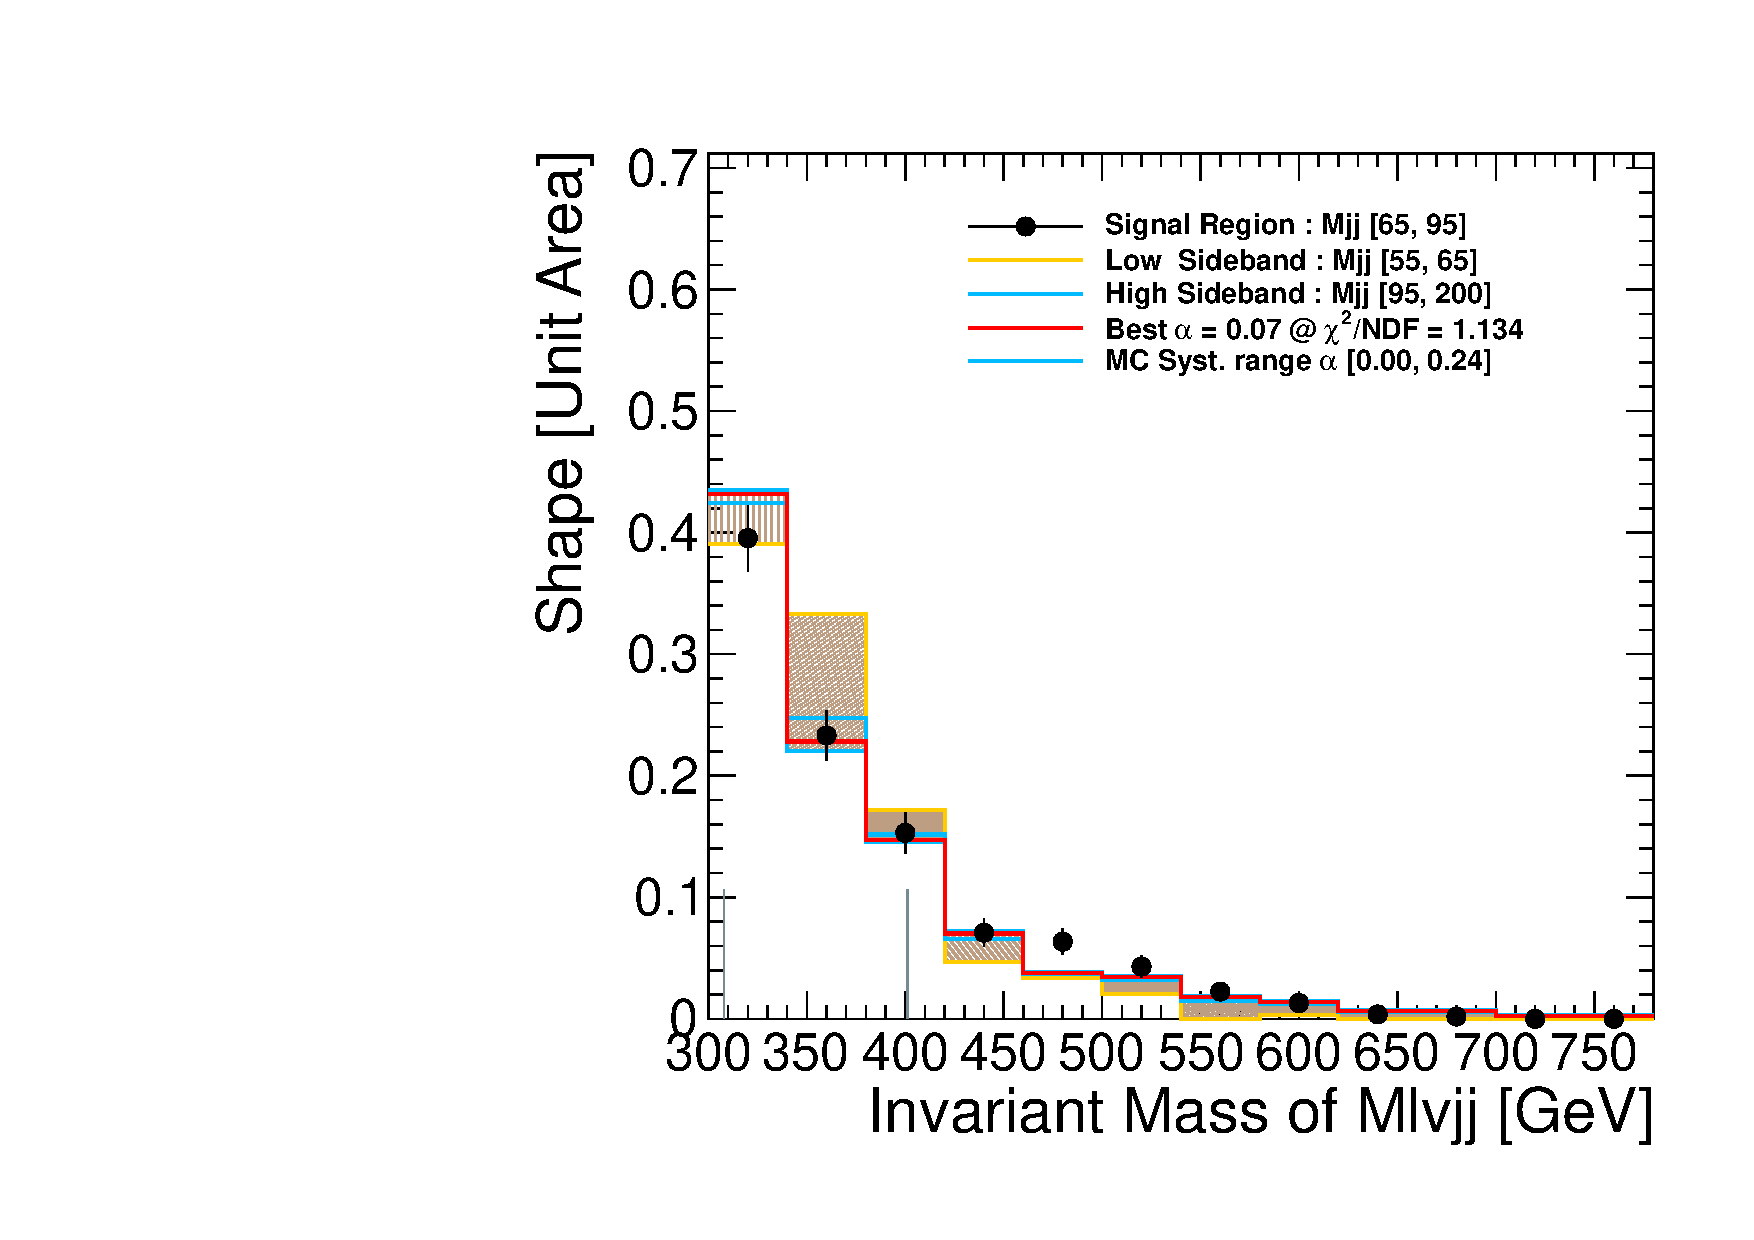
\includegraphics[width=0.49\textwidth]{plots/anaexample/2j350mu-Alpha-mcget-MVAgt_60_Range_12_300-780_SB_55-65_95-200.pdf}
  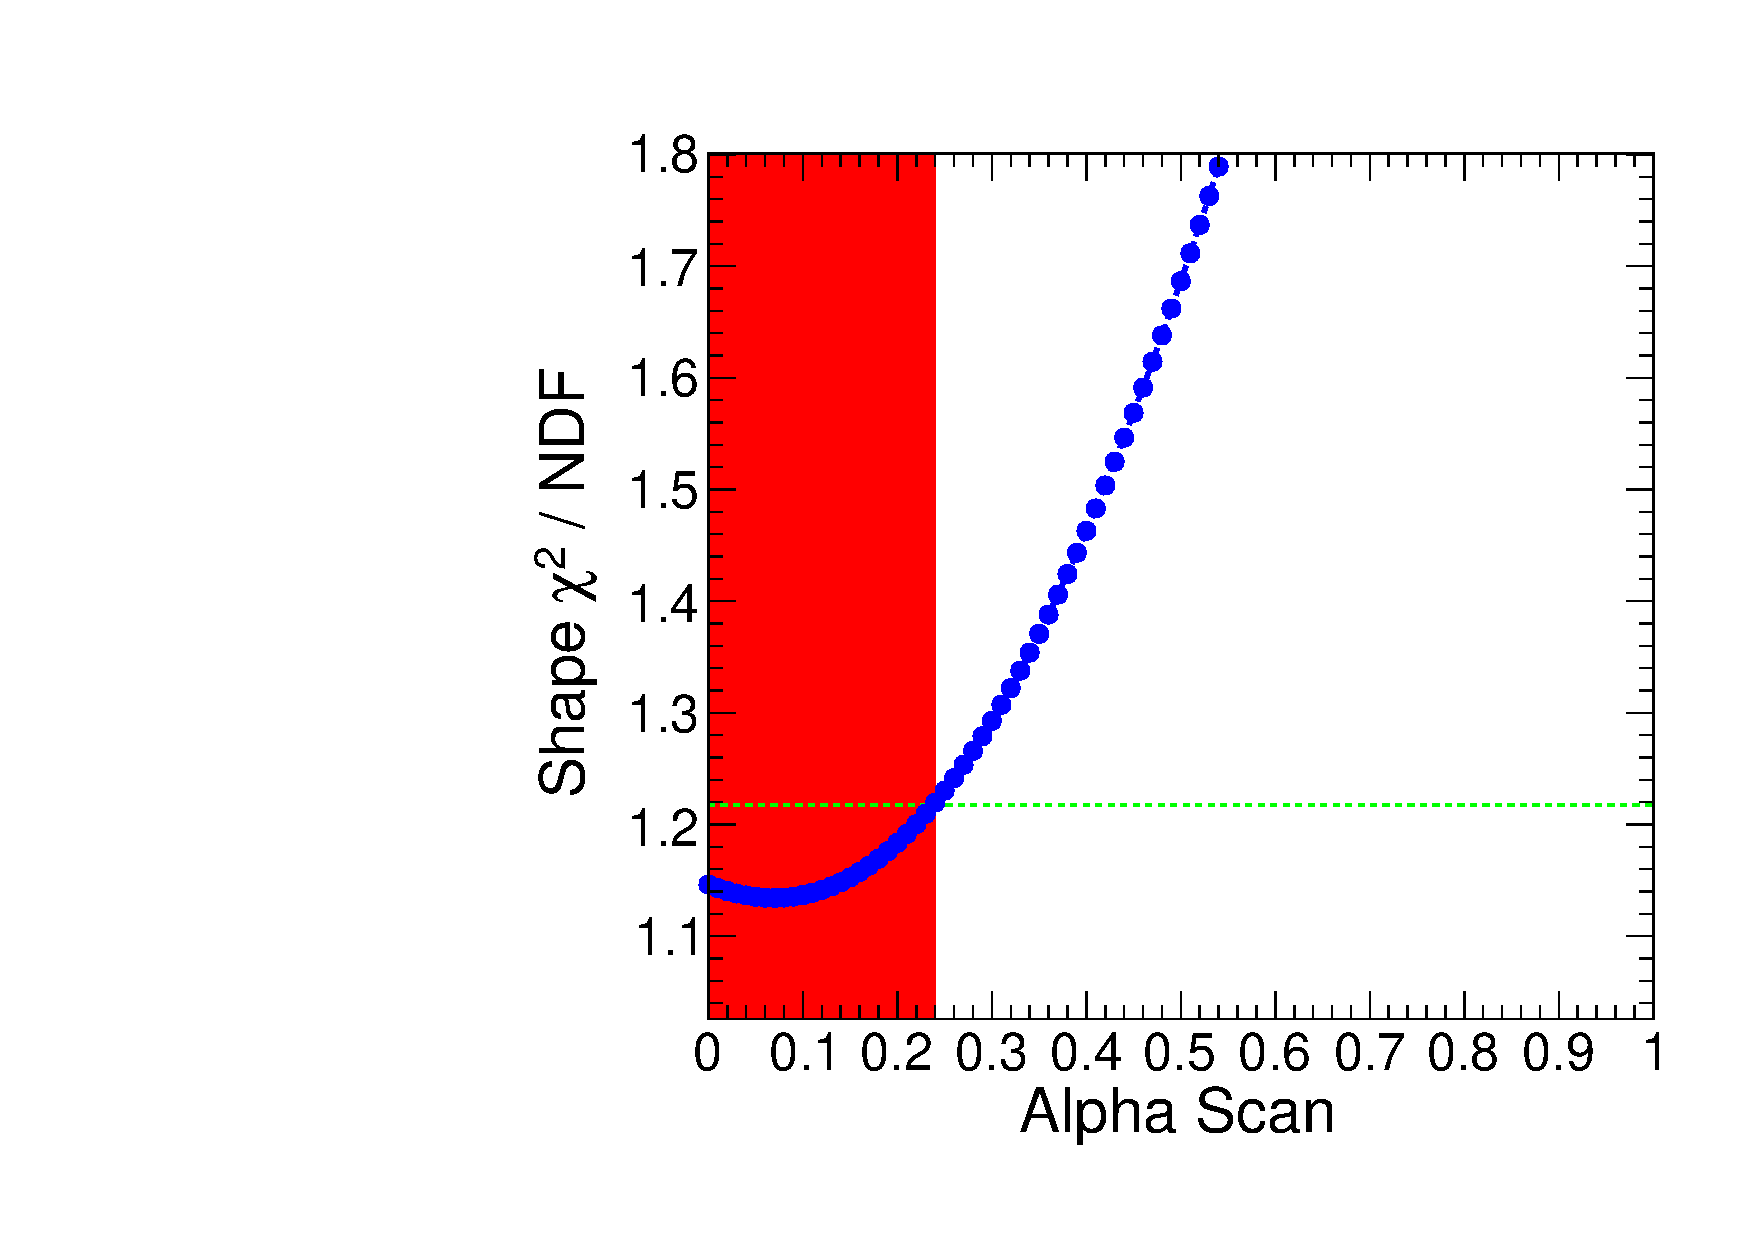
\includegraphics[width=0.49\textwidth]{plots/anaexample/2j350mu-Alpha-mcsca-MVAgt_60_Range_12_300-780_SB_55-65_95-200.pdf}
  \caption{\label{fig:mcalphacheck_2j350mu}The optimal alpha value
    from $W+$jets MC for the SM Higgs mass of 350~GeV for the 2-jet
    $W\to\mu\nu$ category.}
\end{figure}
%

\subsection{Determination of the normalization from fits to dijet mass}
\label{sec:mjjfitfornormal}
% .... .... .... .... .... .... .... .... .... .... .... .... .... .... .... .... .... .... .... .... .... .... ....

We extract the background yields from an unbinned maximum likelihood
fit to the dijet invariant mass distribution $m_{jj}$, after the selection on the MVA discriminant,
excluding the signal region ($65~{\mbox{GeV}} < m_{jj} < 95~{\mbox{GeV}}$). 
% Events in the signal region are later used to set Higgs exclusion limits. 
In this fit, all the backgrounds are considered. 
The W+jets shape is described as described in Section~\ref{sec:wjetsShape},
the QCD shape as described in Section~\ref{sec:dataDrivenQCD}, 
while the other background shapes come from the simulation.
The dijet mass spectrum fit fixes therefore the yields of the physics processes. 
Table~\ref{tab:mjj_shapes_and_normalization} shows in a schematic view how the 
shape of each component is determined, and what constraints 
are applied to fit for the normalization. 

\begin{table}[!ht]
  \begin{center}
 \caption{Determination of the $m_{jj}$ shape and normalization.}  
 \label{tab:mjj_shapes_and_normalization} 
 \begin{tabular} {l  c  c c c }
   \hline \hline
   Process                &    Shape                         &  Shape syst.           & Normalization   &  Norm. syst.\\  \hline
   W+jets                 &    data                      &  ---  & Unconstrained   &  Unconstrained \\
   diboson                &    MC                            &  JES                   & Constrain: NLO        &  Gauss $\sigma =10\%$ \\ 
   $t\bar{t}$ &    MC                            &  JES                   & Constrain: NLO        &  Gauss $\sigma =6.3\%$  \\ 
   single top & MC & JES & Constrain:NLO & Gauss $\sigma=5\%$ \\
   Z+jets                 &    MC                            &  JES                   & Constrain: NLO        &  Gauss $\sigma =4.3\%$  \\
   QCD                    &    data                          &  JES                   & Constrain: MET fit in data  &  Sec.~\ref{sec:qcd_Uncertainty}  \\\hline \hline
 \end{tabular}
\end{center}
\end{table}


%% The resulting fit for the SM Higgs mass of 350~GeV for the 2-jet
The resulting fit for the SM Higgs mass of 300~GeV for the 2-jet
$W\to\mu\nu$ category is shown in Figs~\ref{fig:mjj_mH350} with the
event yields of the different physics processes and the chisquared of
the fit. 
The electroweak diboson yield is robustly determined with the expected mean mass and mass resolution. 

\begin{figure}[!t]
  \centering
%%  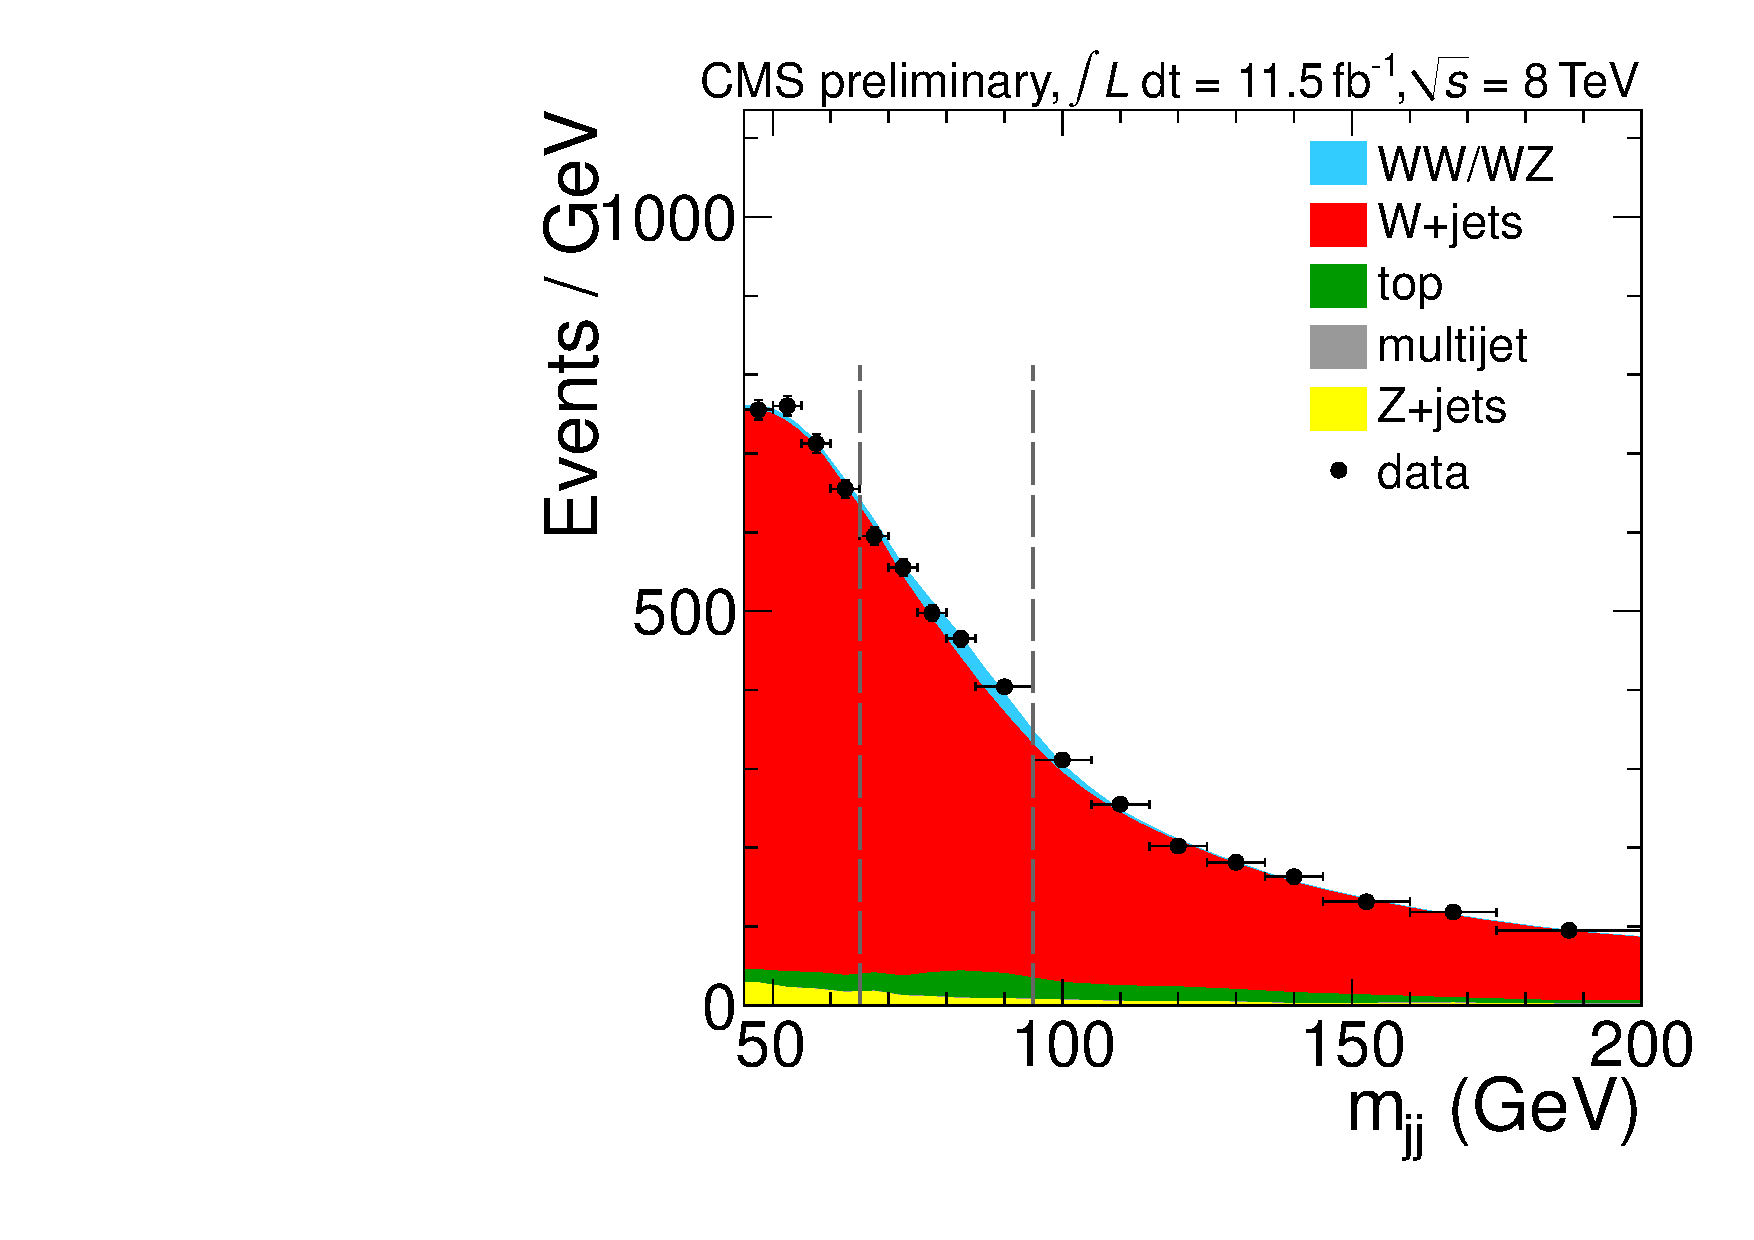
\includegraphics[width=0.49\textwidth]{plots/anaexample/H350_Mjj_Muon_2jets_Stacked}
%%  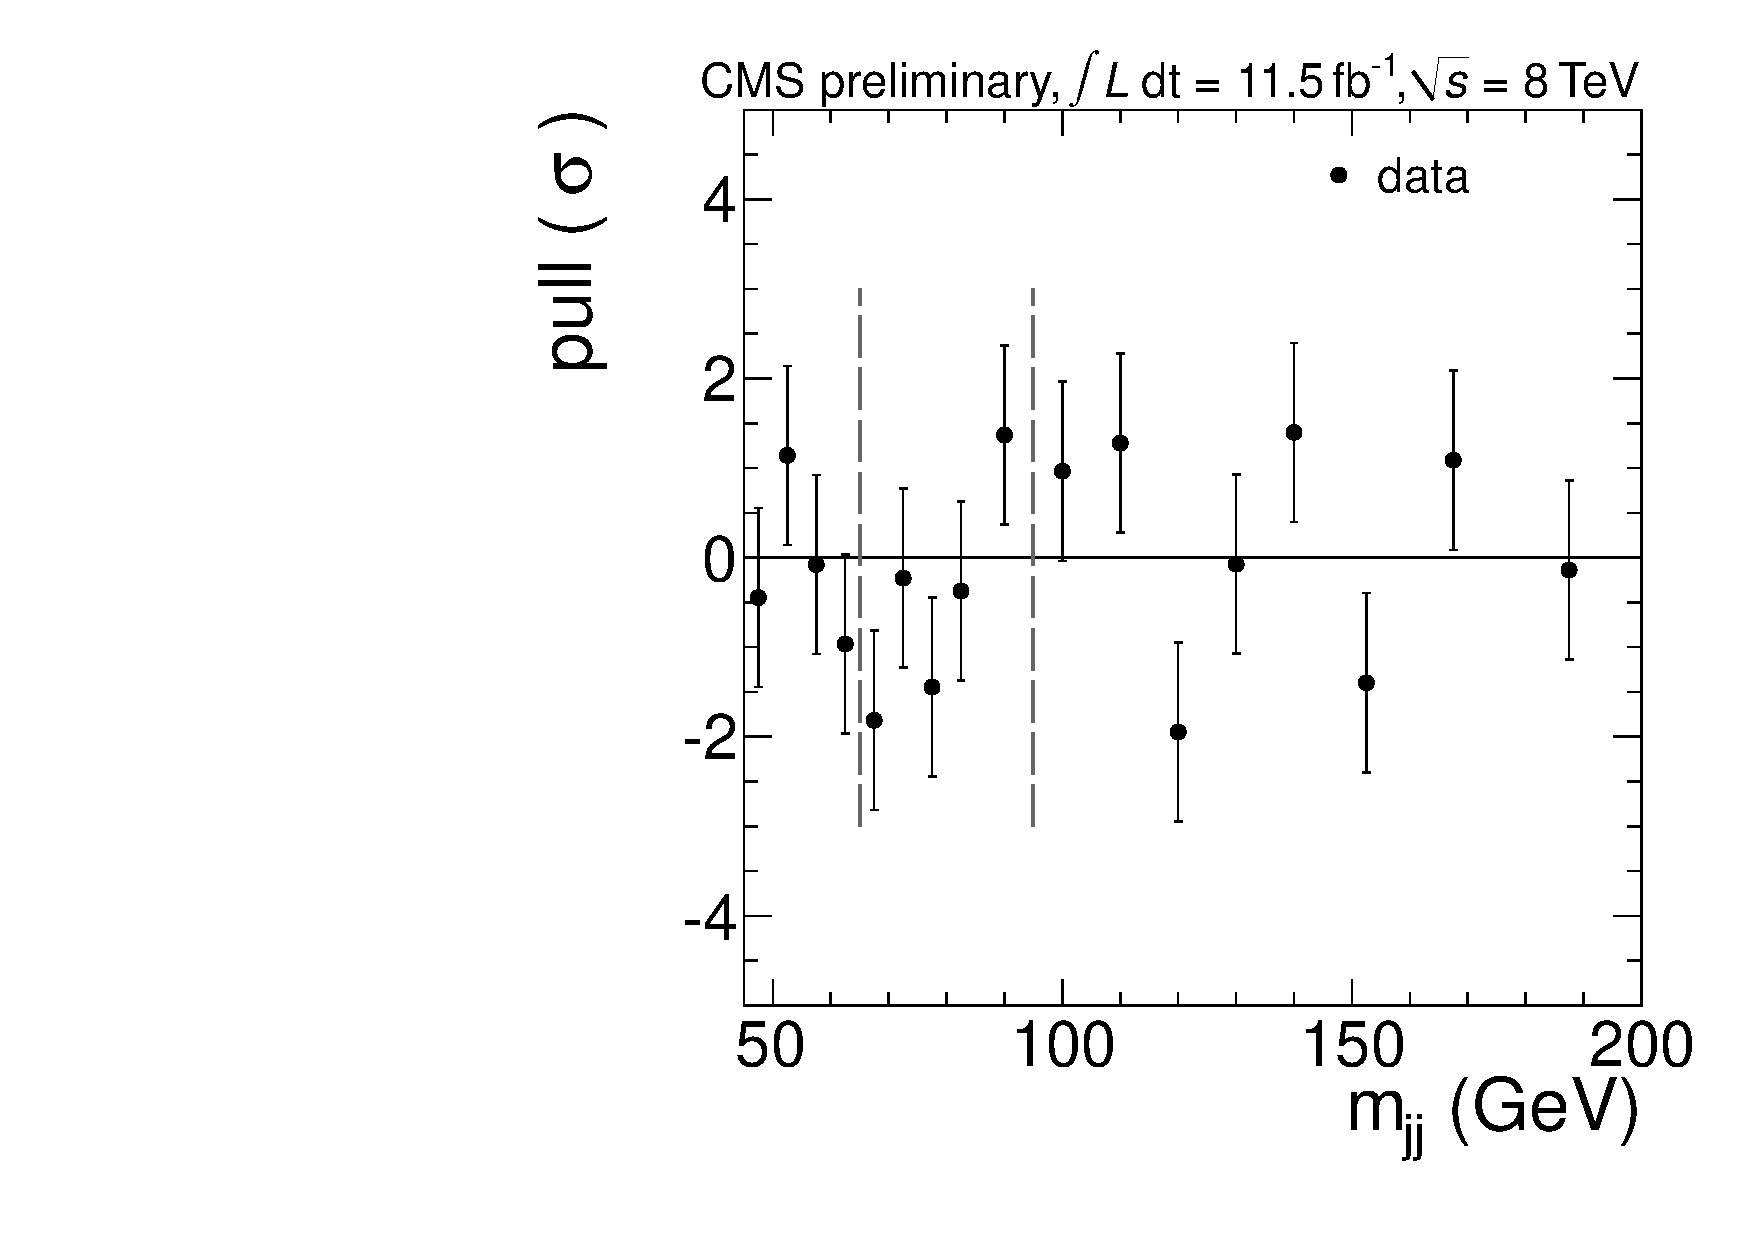
\includegraphics[width=0.49\textwidth]{plots/anaexample/H350_Mjj_Muon_2jets_Pull}
  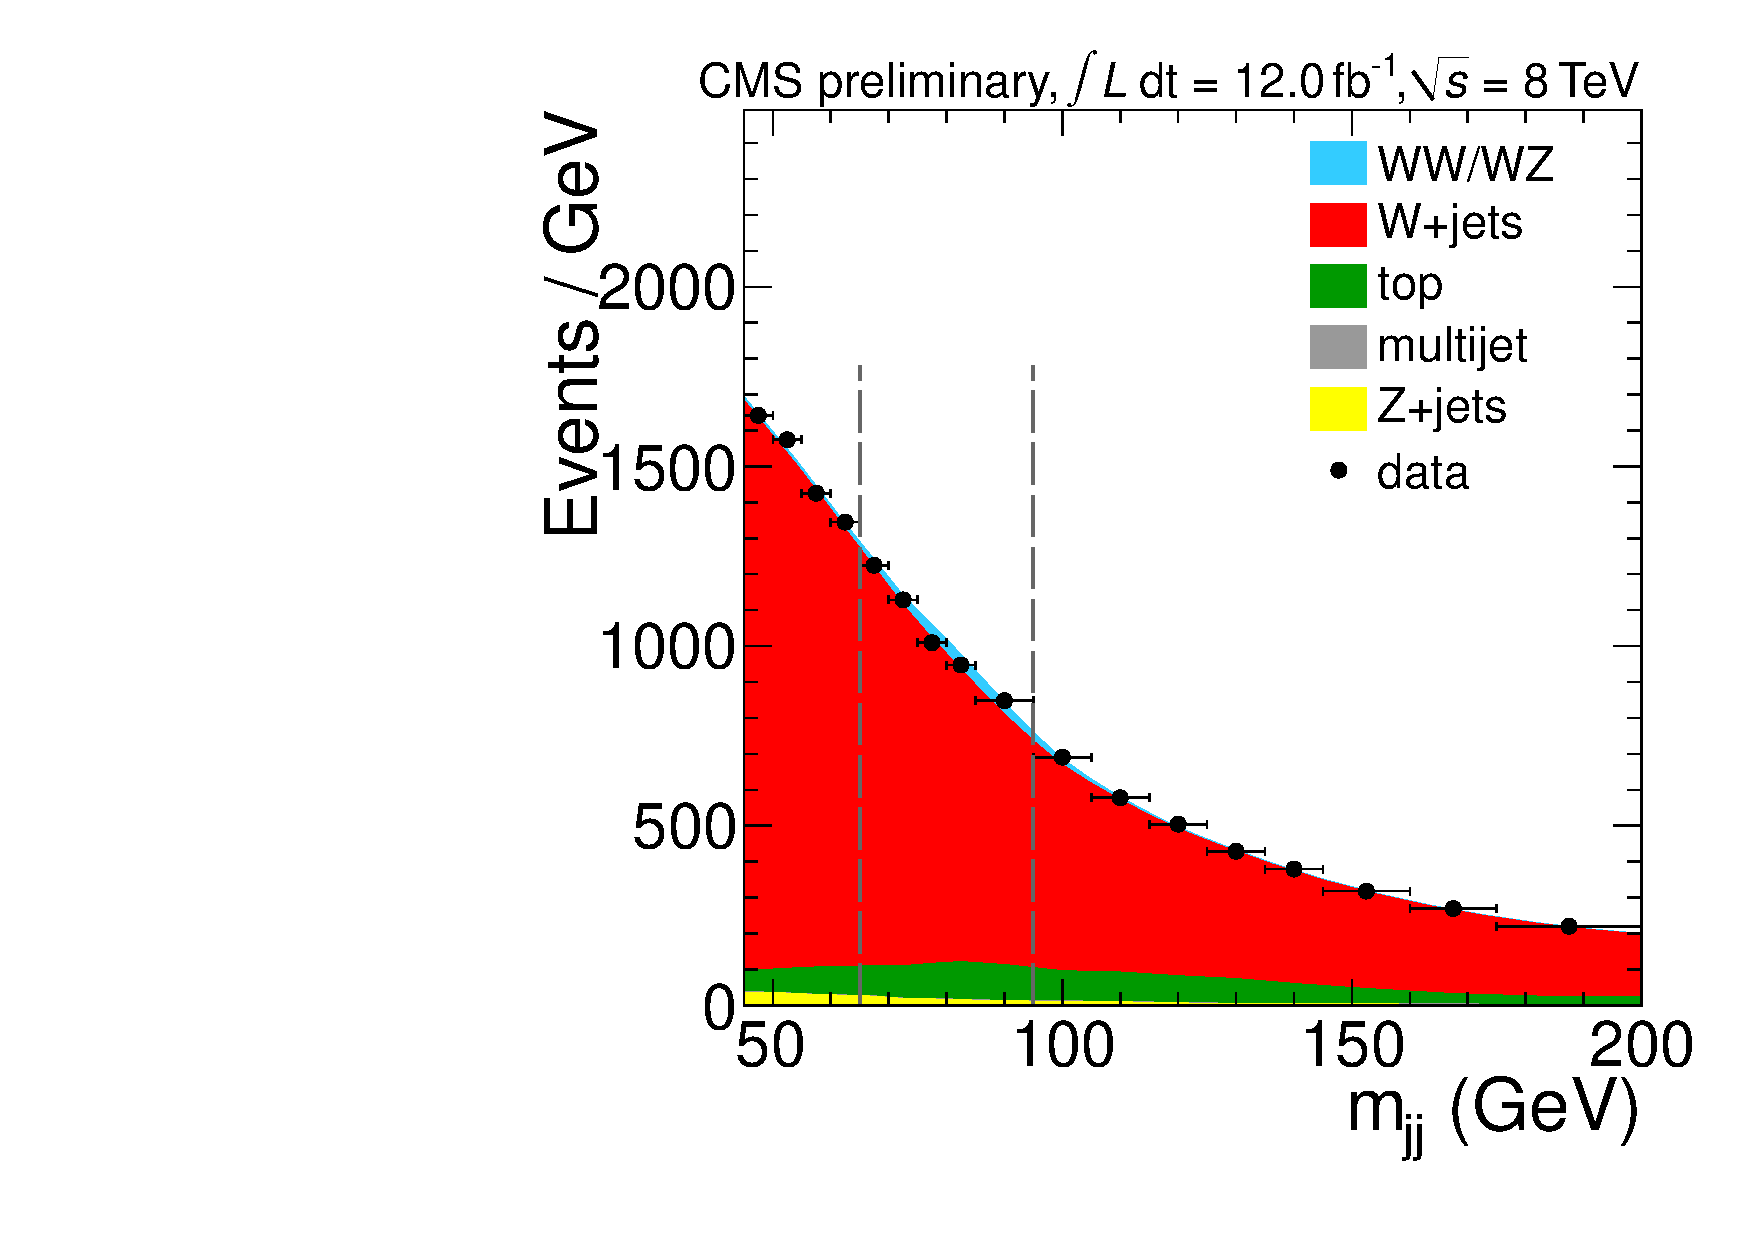
\includegraphics[width=0.49\textwidth]{plots/anaexample/H300_Mjj_Muon_2jets_Stacked}
  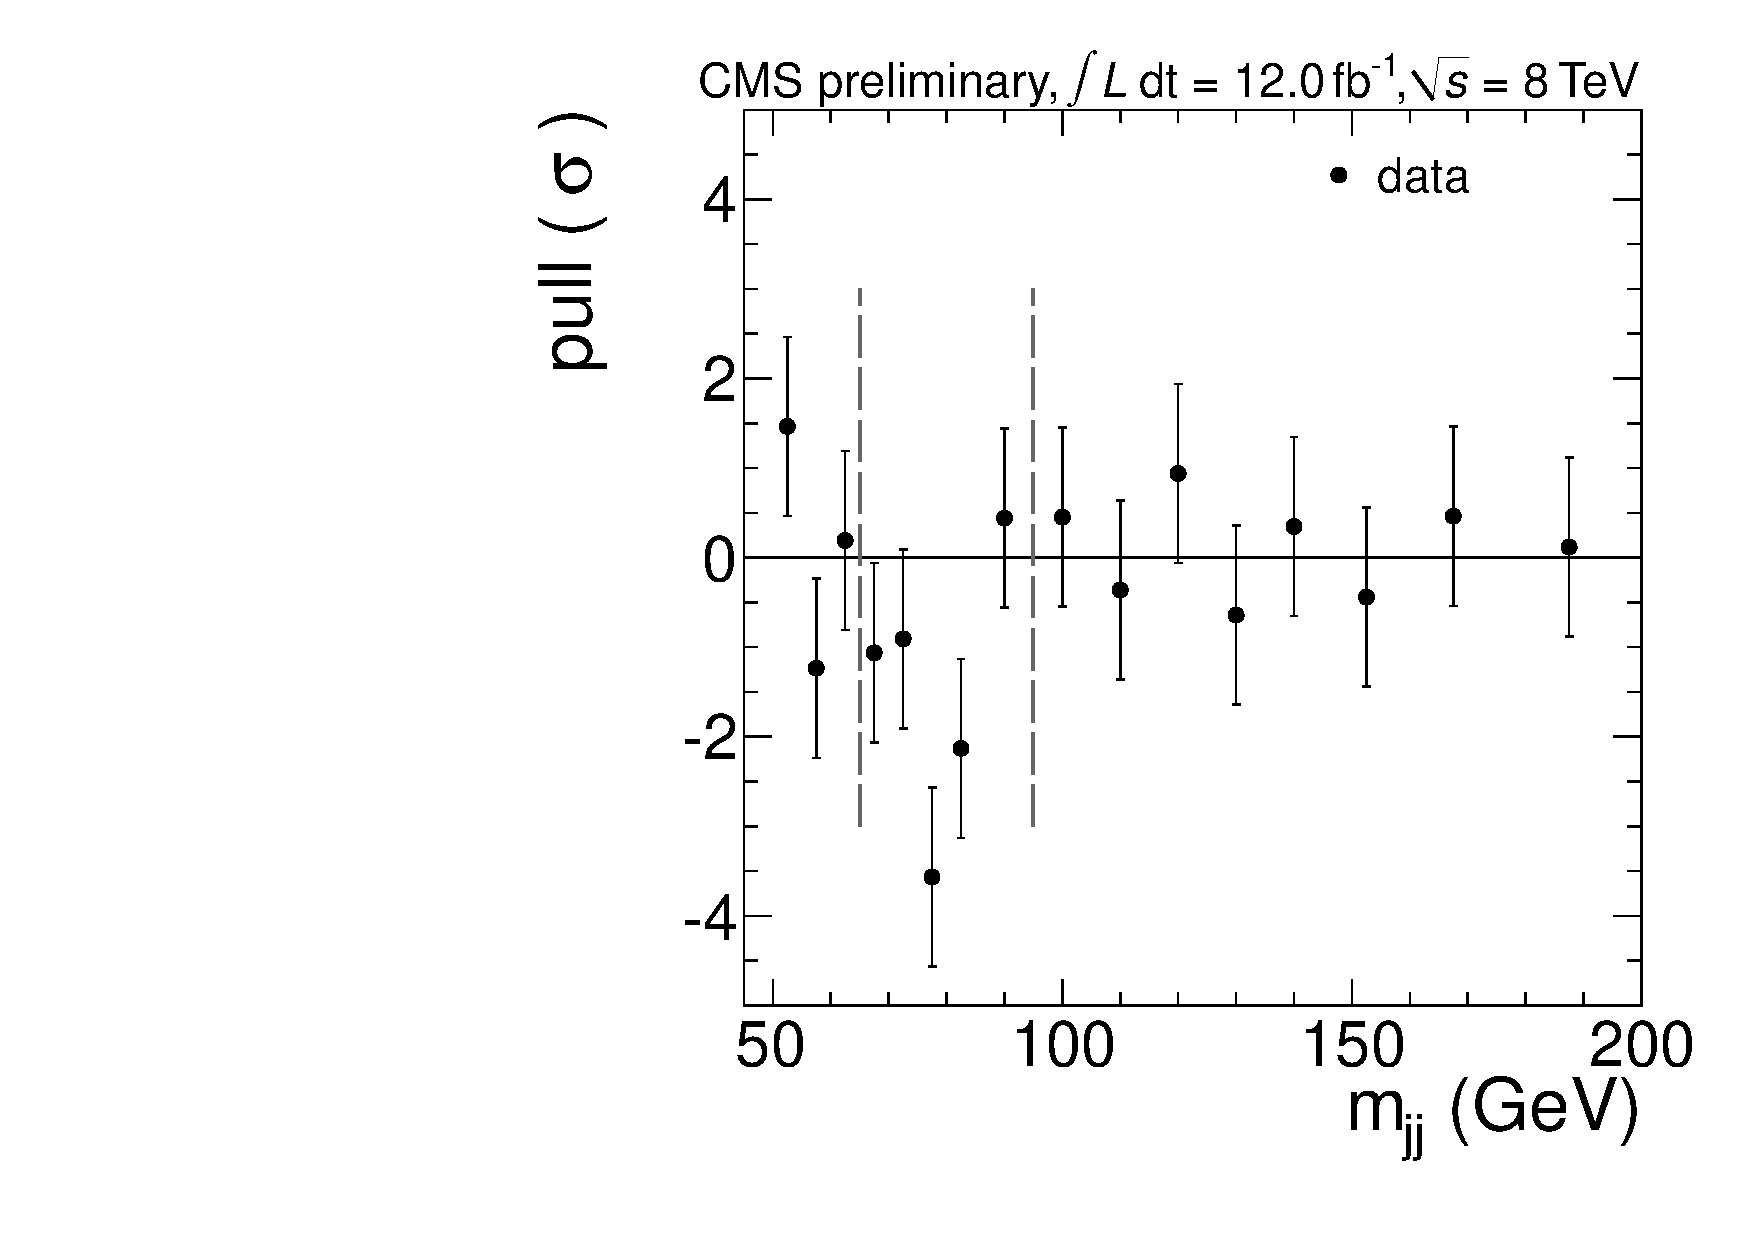
\includegraphics[width=0.49\textwidth]{plots/anaexample/H300_Mjj_Muon_2jets_Pull}
  \caption{\label{fig:mjj_mH350}For the SM Higgs mass of
%%  350~GeV for the 2-jet $W\to\mu\nu$ category, the distribution of
    300~GeV for the 2-jet $W\to\mu\nu$ category, the distribution of
    the dijet invariant mass $m_{jj}$ is shown on the left. The pull
    distribution computed as [(Data - Fit)/ Fit uncertainty] is shown
    on the right. } %% The signal region is blinded.}
\end{figure}


\subsection{Use of four-body mass to extract Higgs limits}
\label{sec:mlvjjforlimit}
% .... .... .... .... .... .... .... .... .... .... .... .... .... .... .... .... .... .... .... .... .... .... ....


Having determined the yield of the ensemble of physics processes using
the Dijet sidebands the four body mass spectrum where the dijet mass
lies in the W mass window is then explored.  For the W+jets
background, the WW four body mass is derived from the four body mass
distributions of the high and low dijet sidebands extrapolated into
the W mass window using the alpha value derived from the Monte Carlo
models as was described in Sec.~\ref{sec:alphaExtraction}.  The W+jets
shape derived from the sidebands is then smoothed with a parametric
fit to an exponential shape, modulated with a turn-on when necessary.
The distribution of the extrapolated W+jets background in the signal
region is reported for four working points in
Figure~\ref{fig:Wjets_dd_example}.  The black dots represent the
extrapolated background, while the red line shows the fitting function
and the blue shaded band the error from the fit.  All other background
categories use the $m_{\ell\nu jj}$ shape predicted by their
respective MC samples.
\begin{figure}[!t]
  \centering
%%     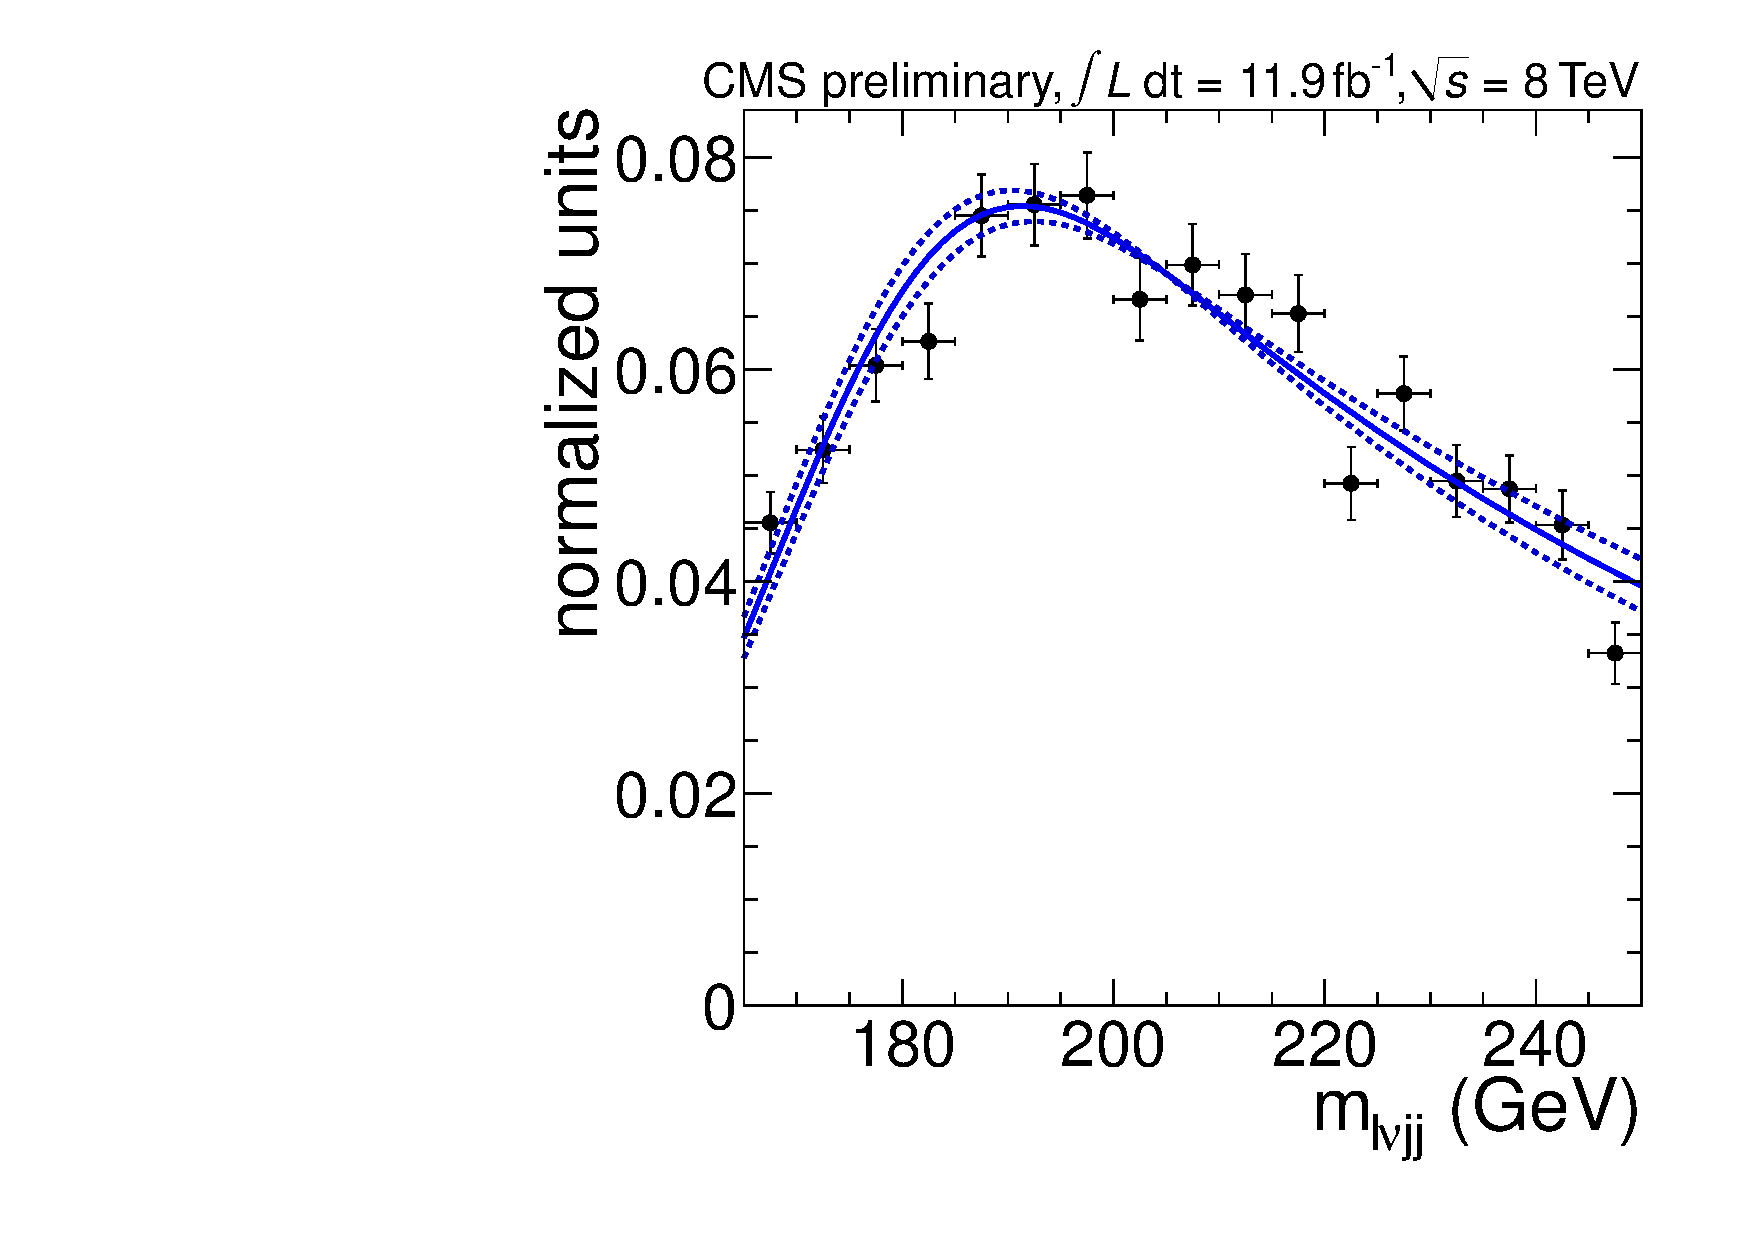
\includegraphics[width=0.45\textwidth]{plots/2012_WJetsShape/H190_Mlvjj_Electron_2jets_WpJShape.pdf}
%%     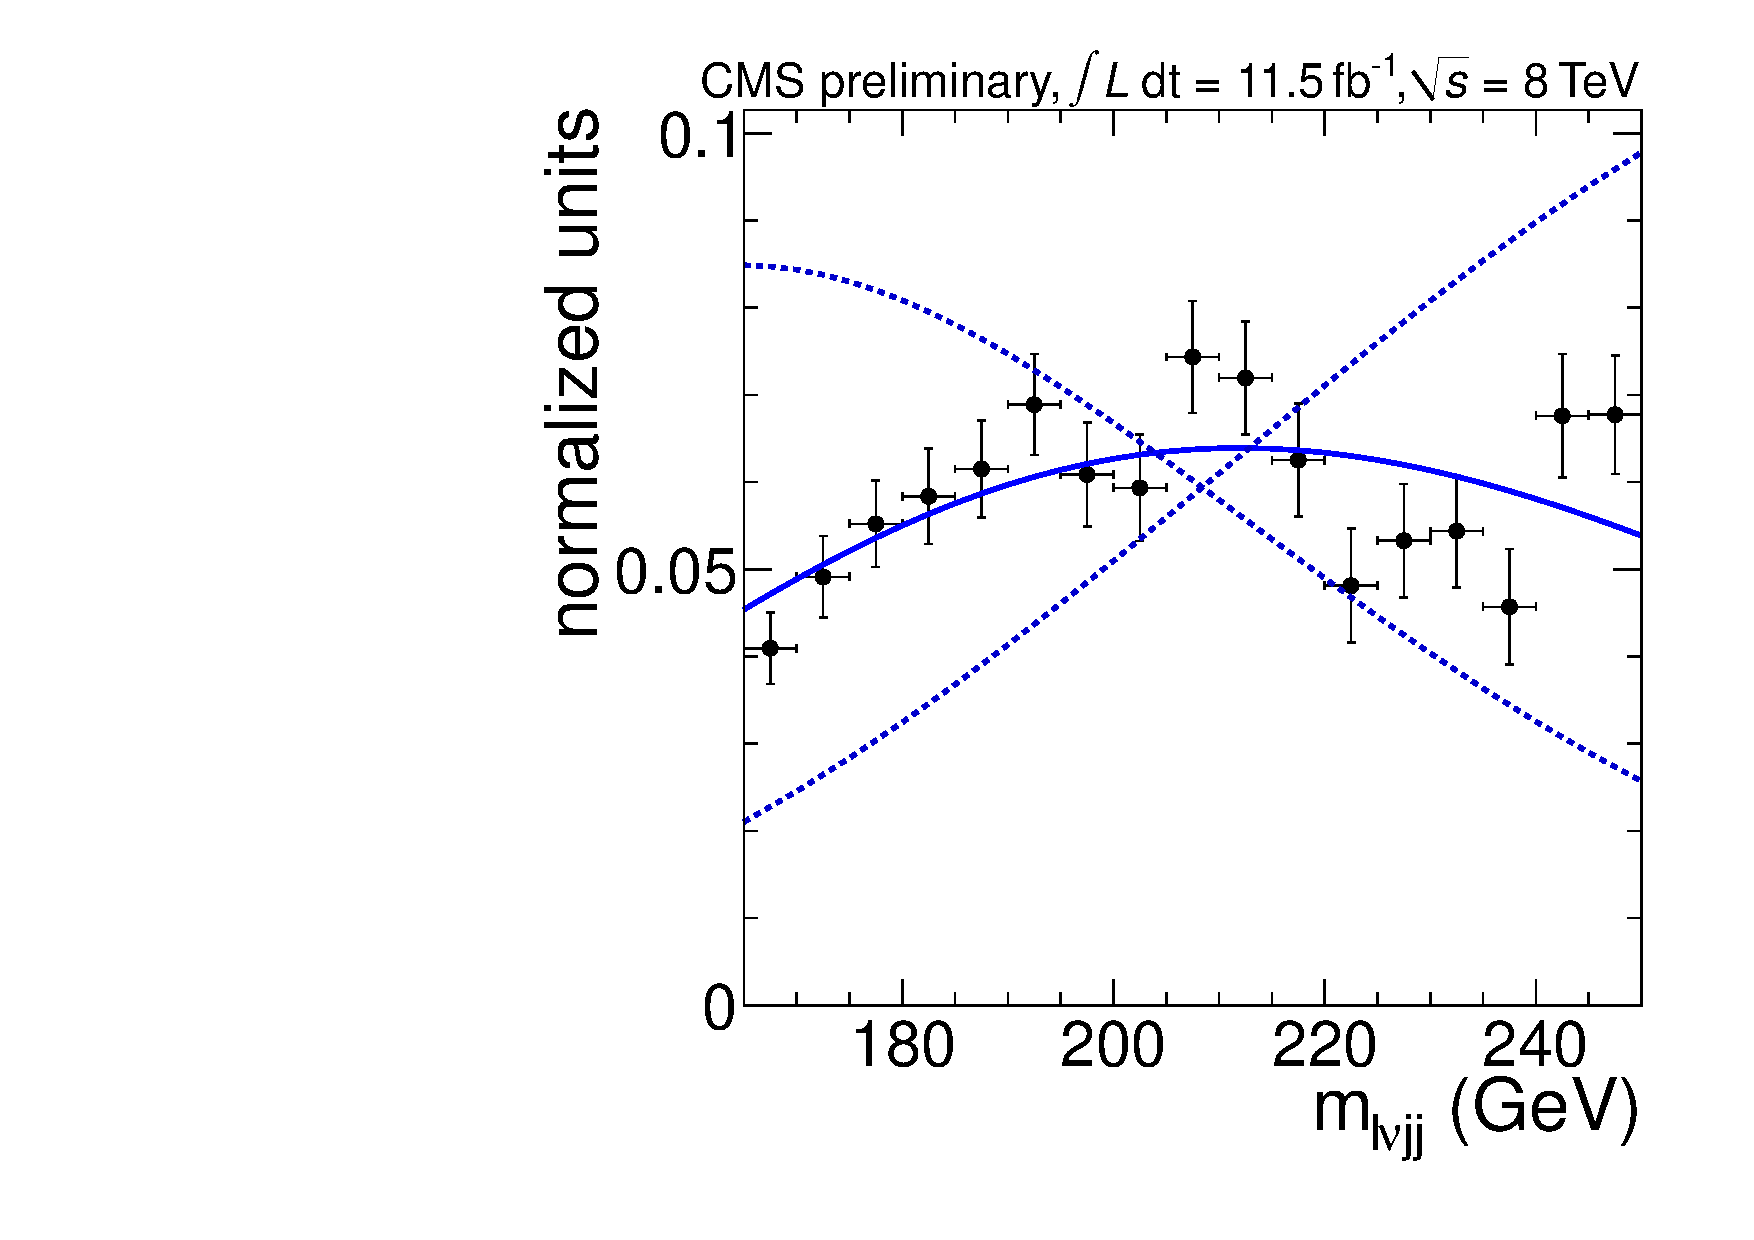
\includegraphics[width=0.45\textwidth]{plots/2012_WJetsShape/H190_Mlvjj_Electron_3jets_WpJShape.pdf}
     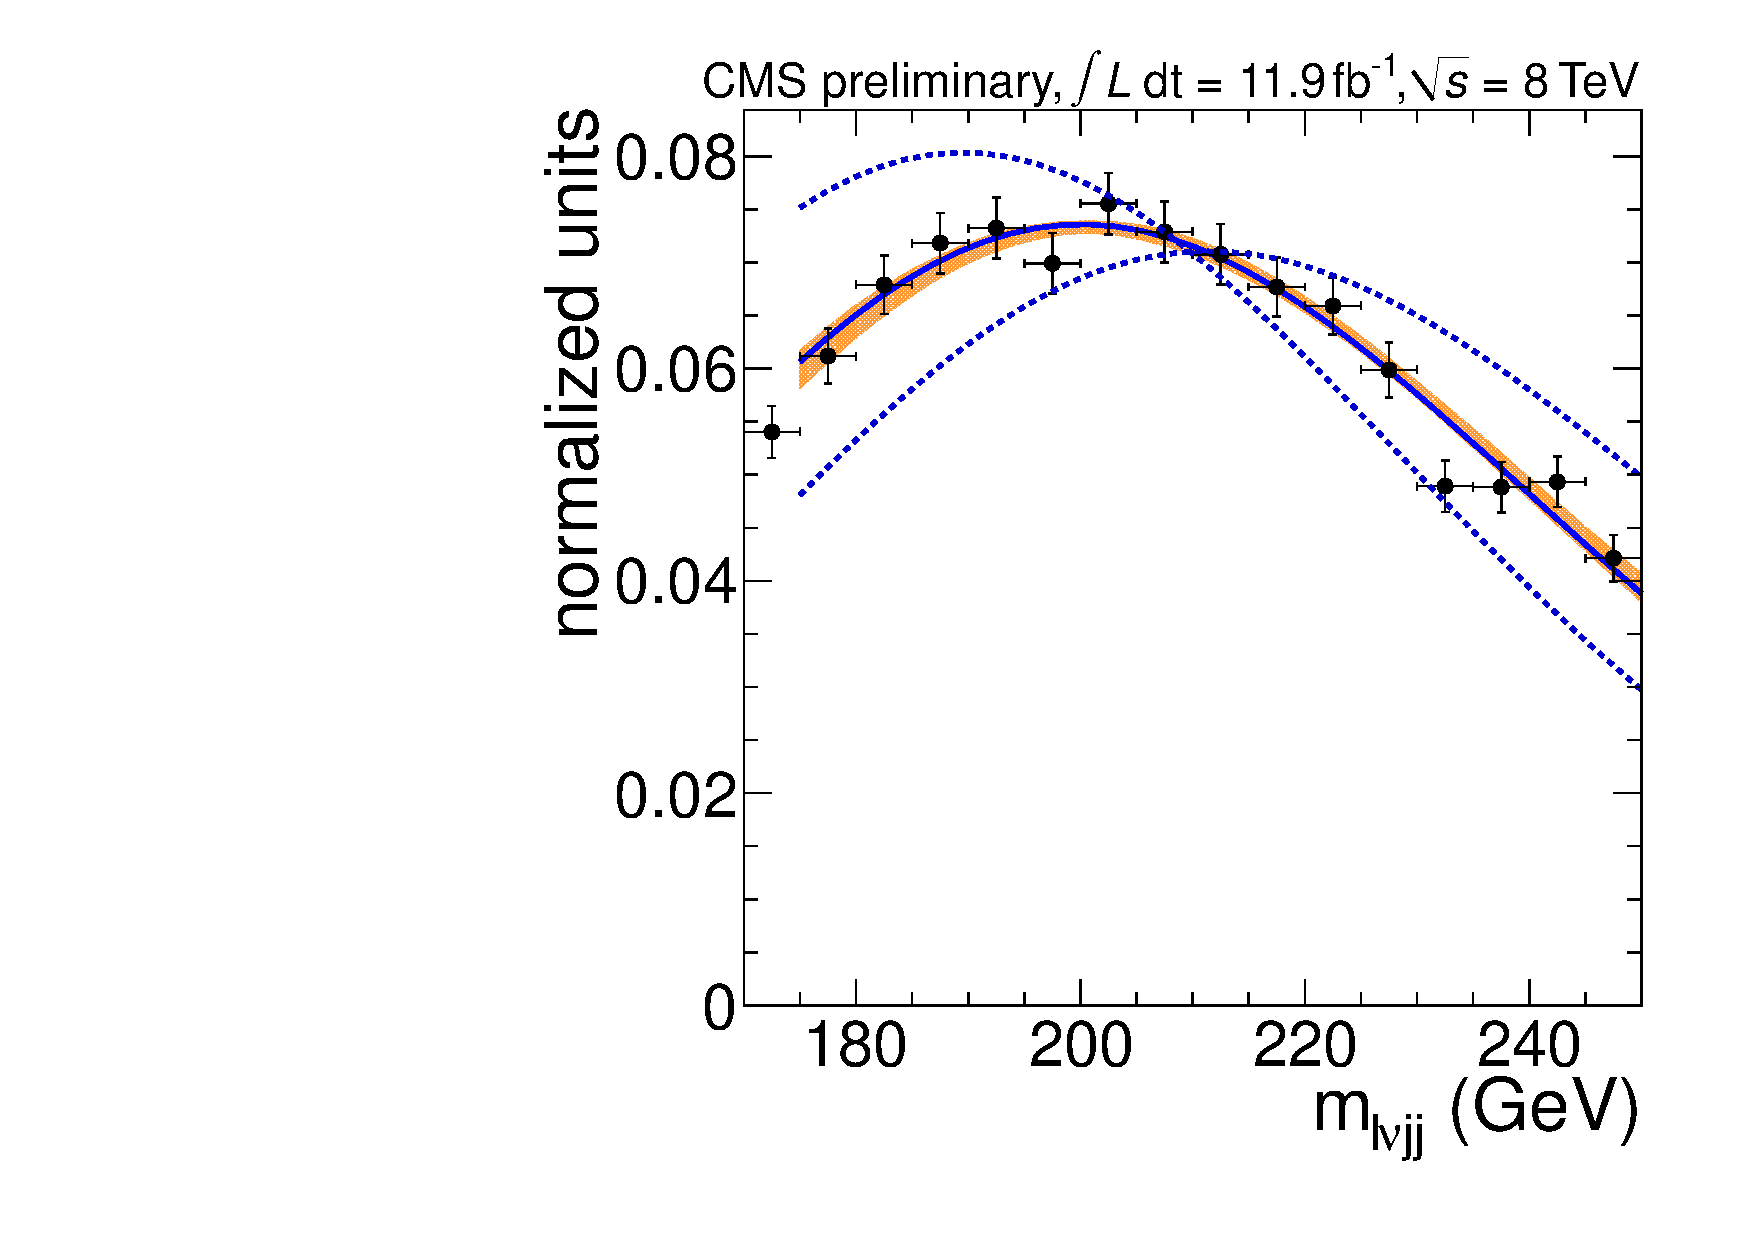
\includegraphics[width=0.45\textwidth]{plots/2012_WJetsShape/H200_Mlvjj_Electron_2jets_WpJShape.pdf}
     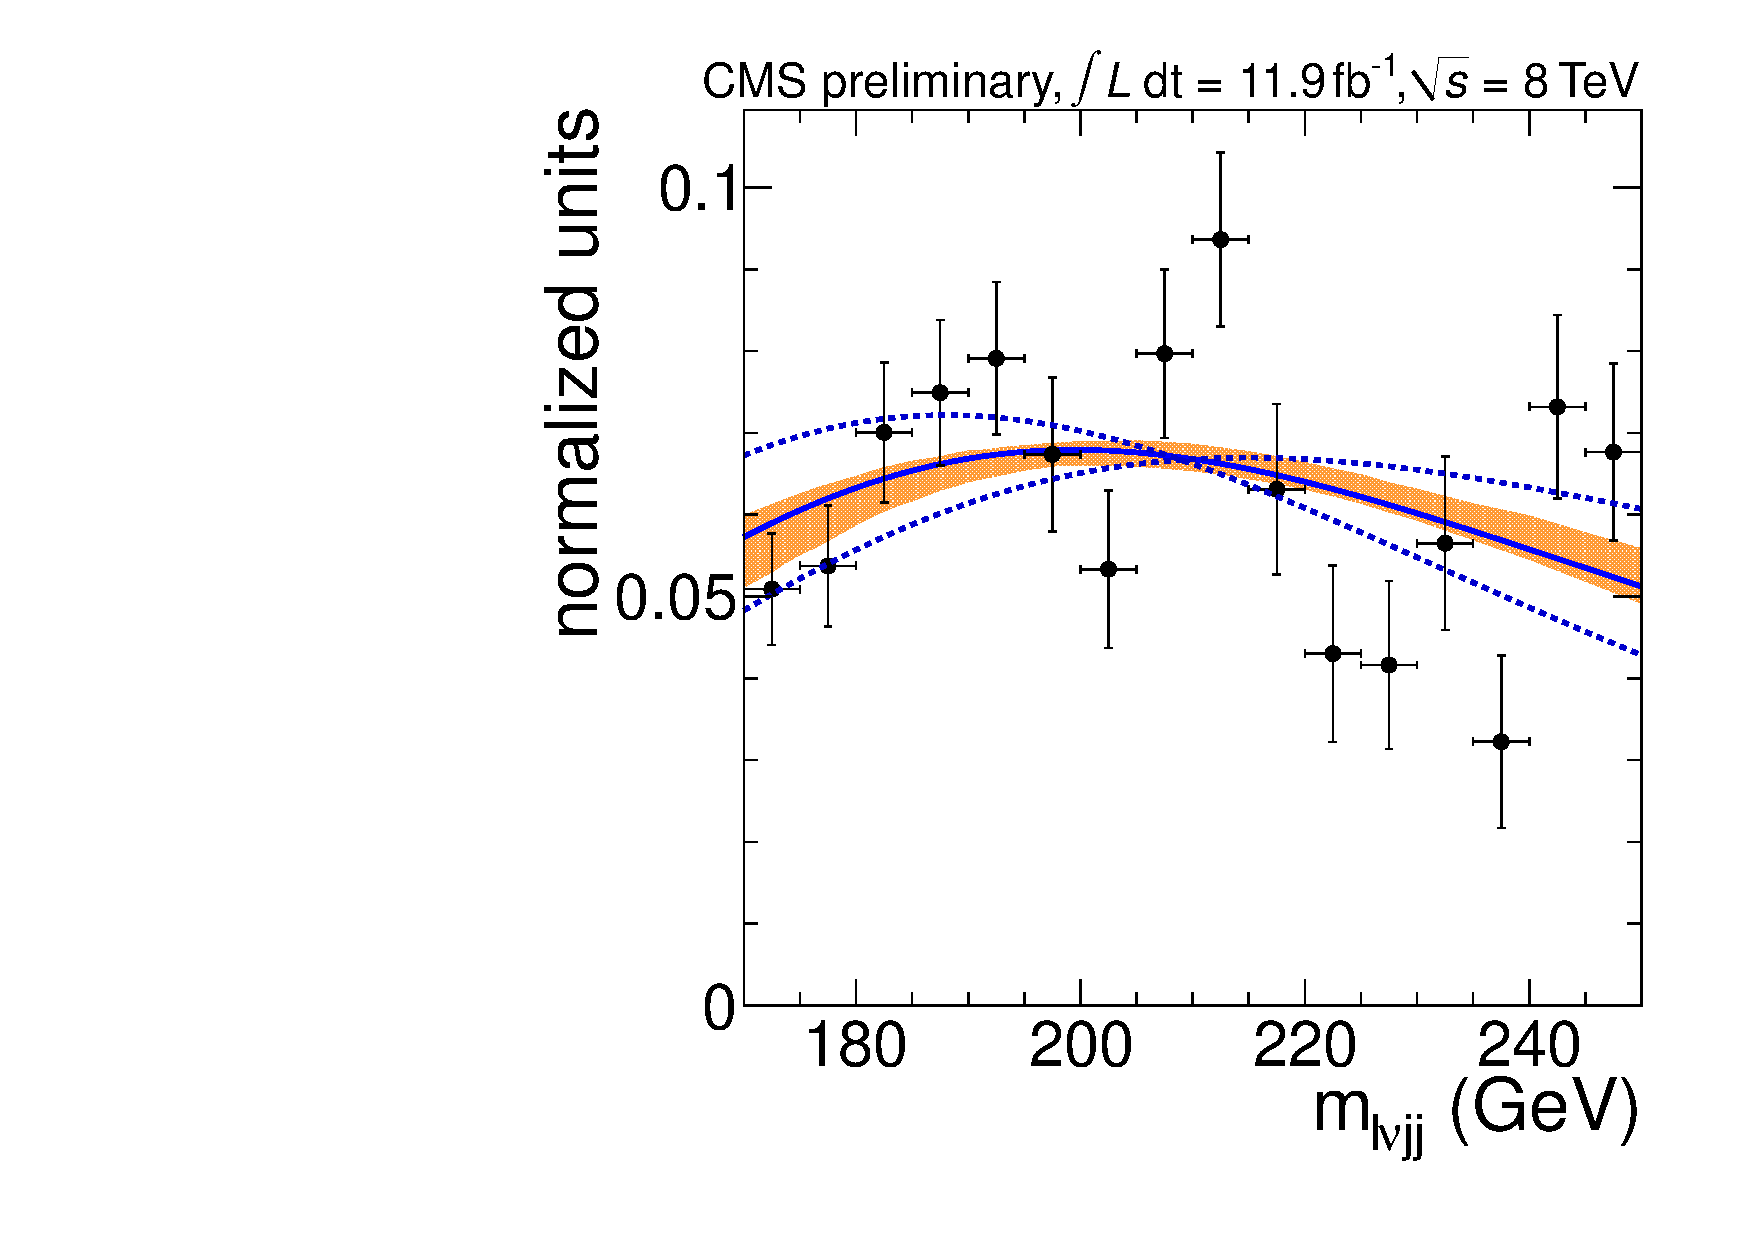
\includegraphics[width=0.45\textwidth]{plots/2012_WJetsShape/H200_Mlvjj_Electron_3jets_WpJShape.pdf}
%%     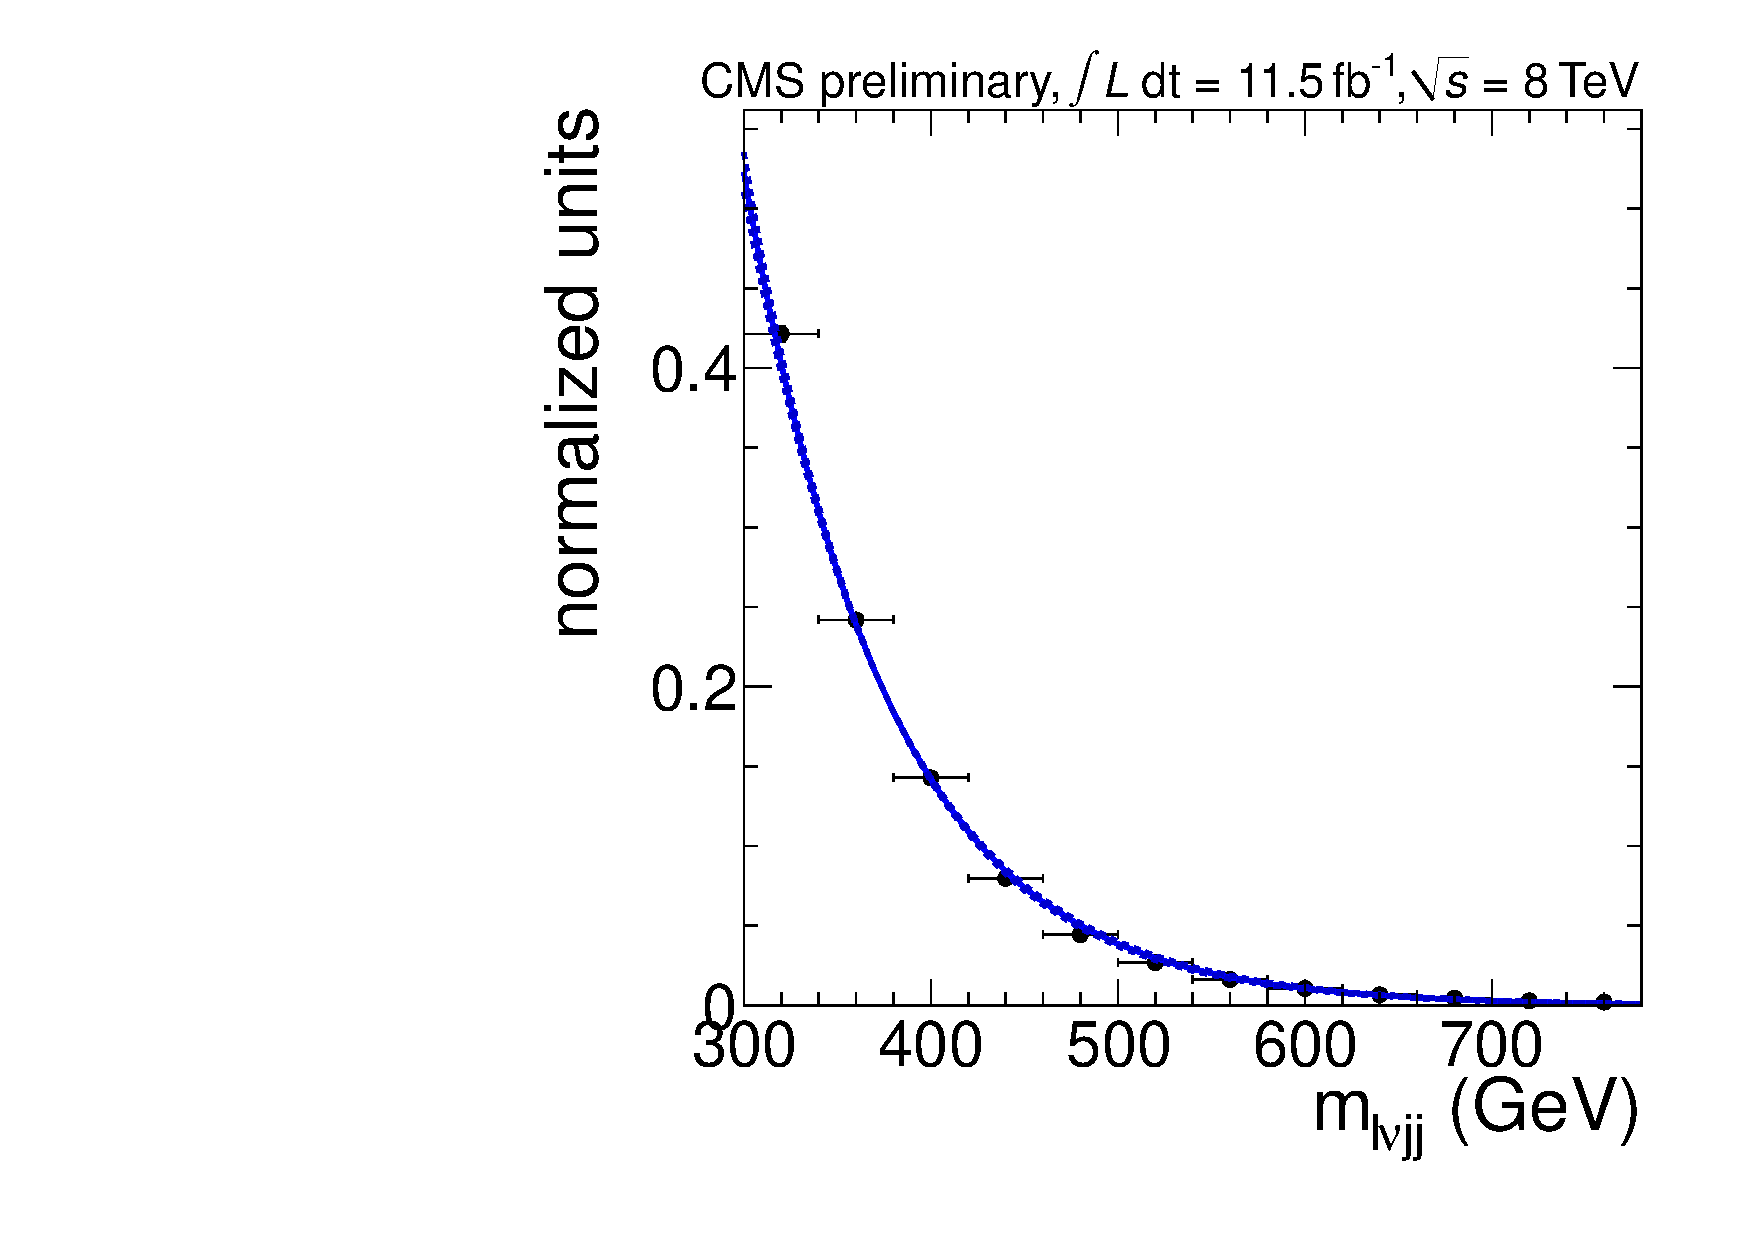
\includegraphics[width=0.45\textwidth]{plots/2012_WJetsShape/H350_Mlvjj_Muon_2jets_WpJShape.pdf}
%%     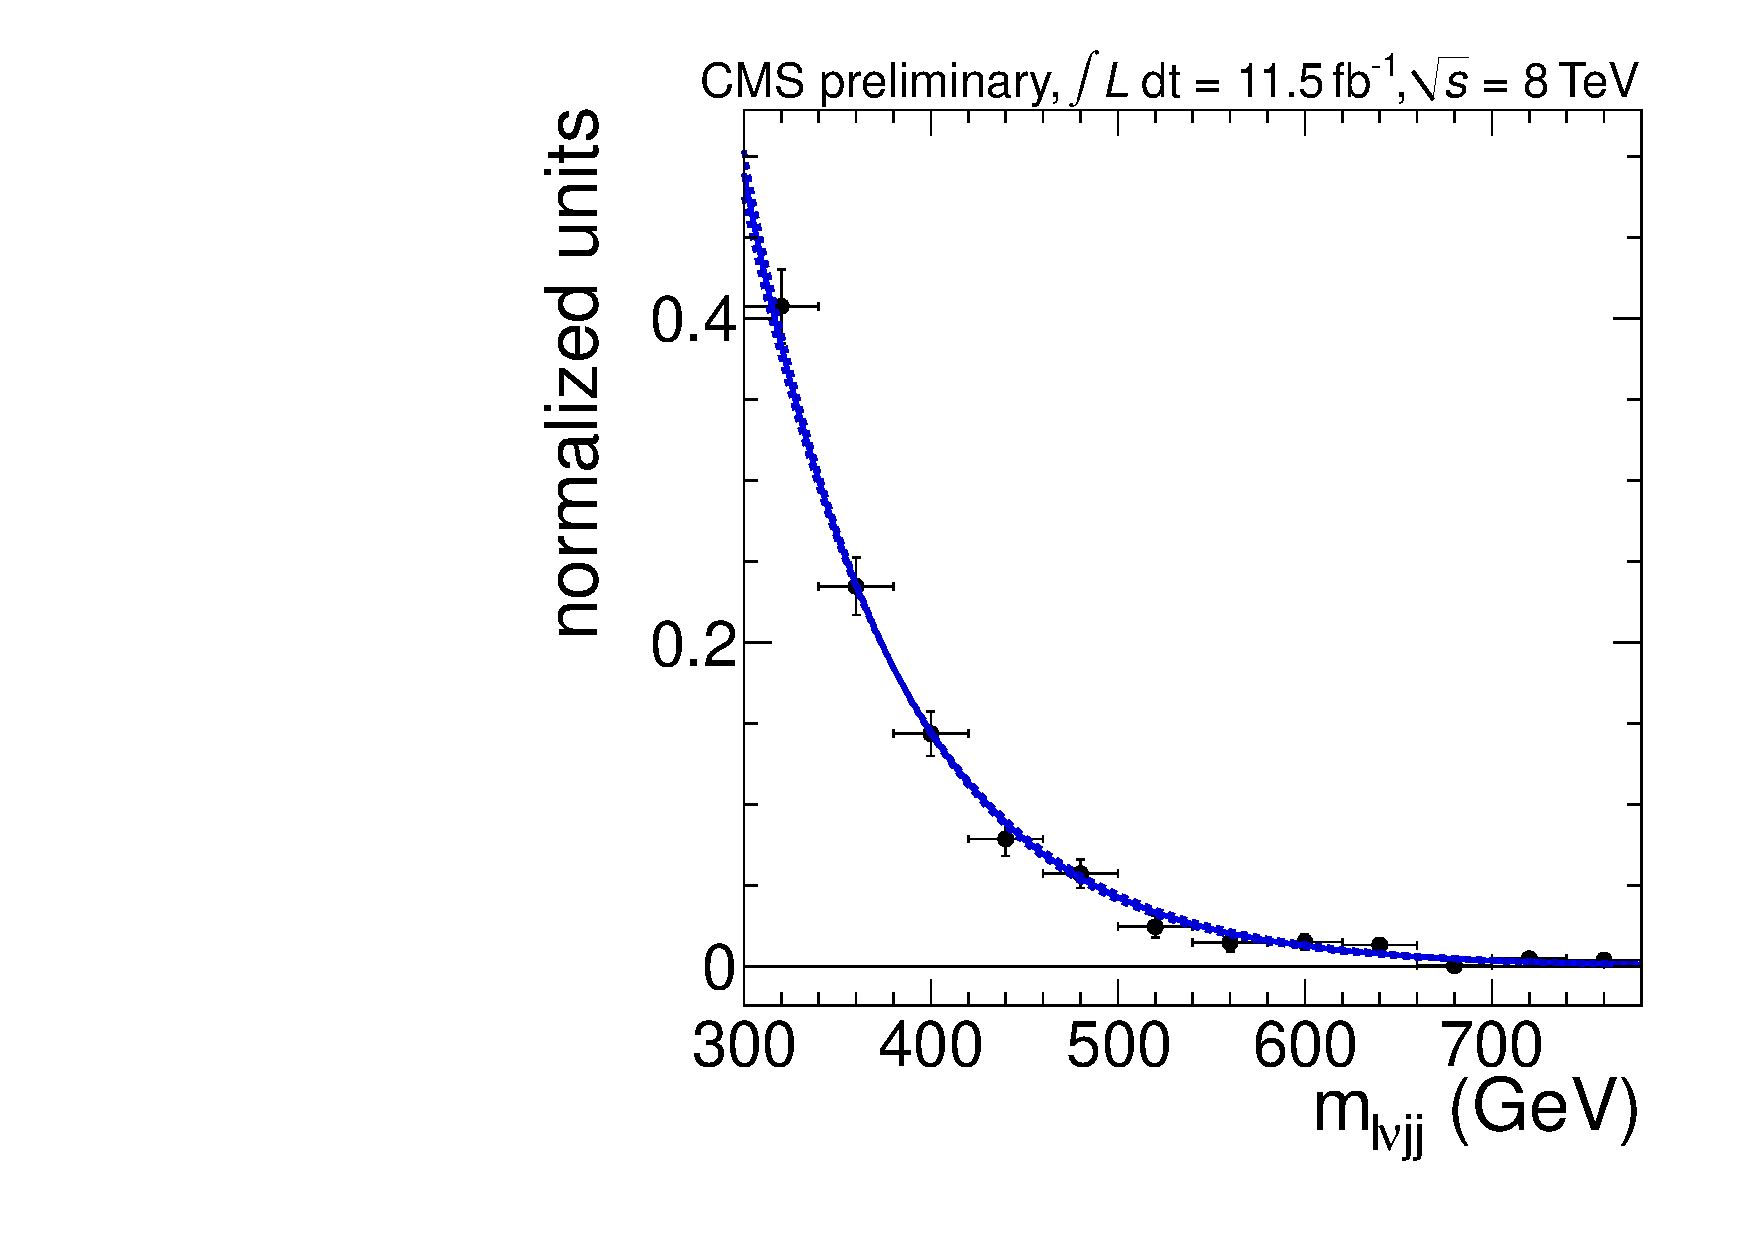
\includegraphics[width=0.45\textwidth]{plots/2012_WJetsShape/H350_Mlvjj_Muon_3jets_WpJShape.pdf}
%%    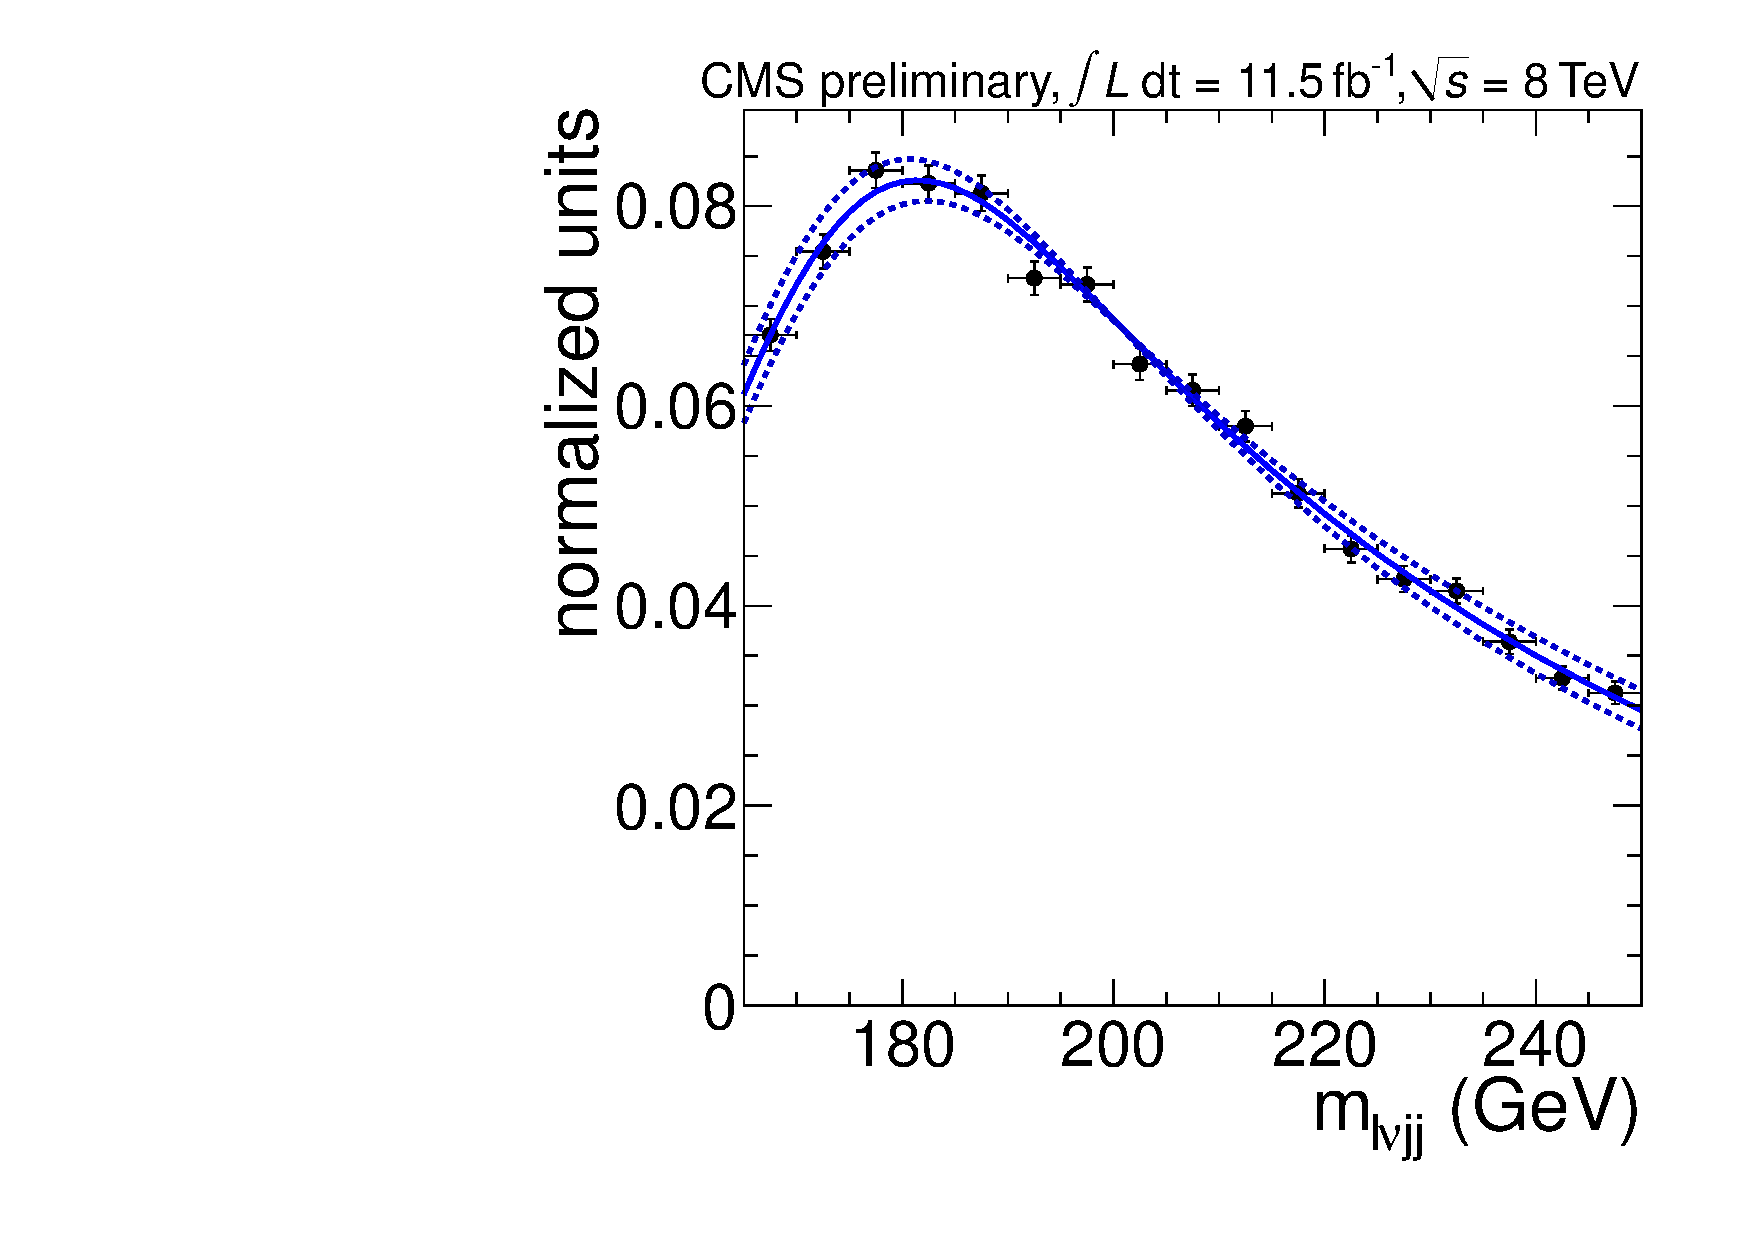
\includegraphics[width=0.45\textwidth]{plots/2012_WJetsShape/H200_Mlvjj_Muon_2jets_WpJShape.pdf}
%%    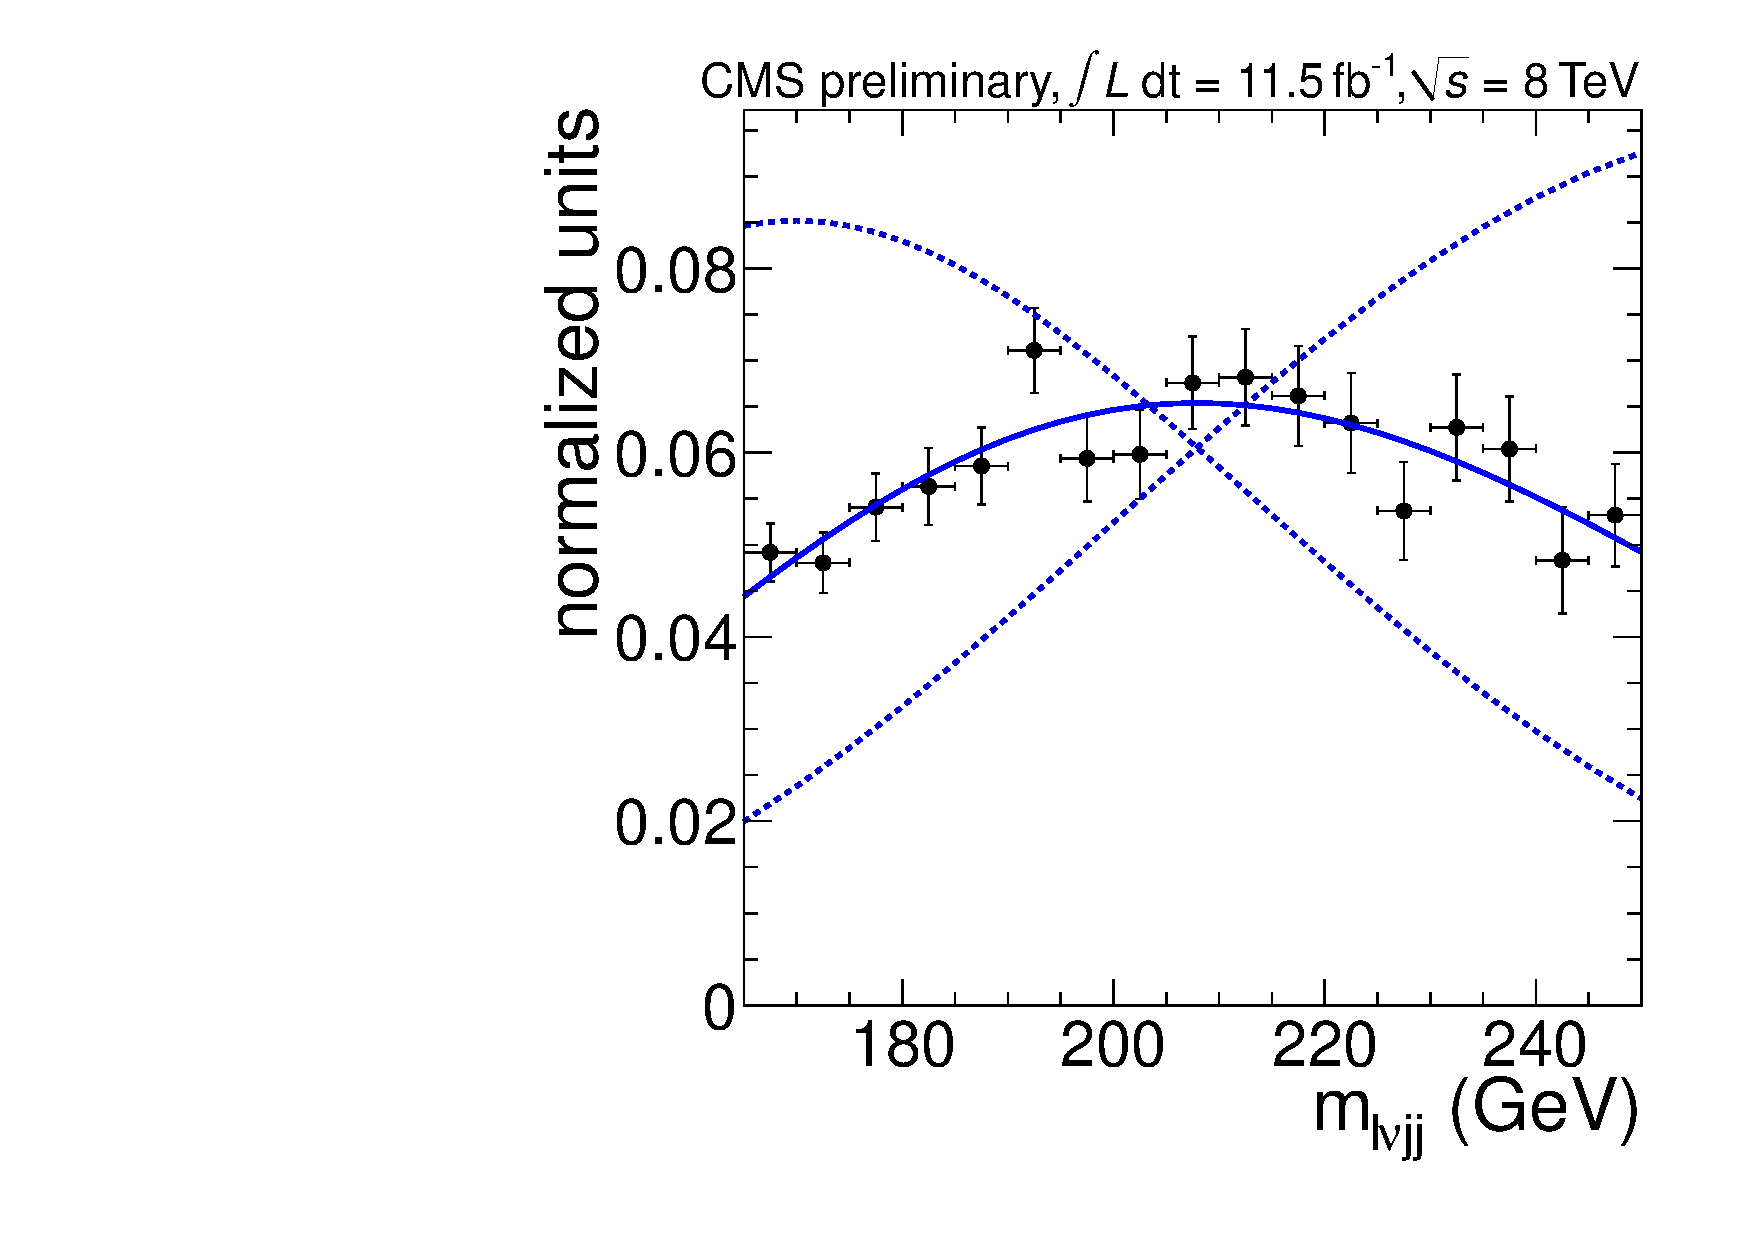
\includegraphics[width=0.45\textwidth]{plots/2012_WJetsShape/H200_Mlvjj_Muon_3jets_WpJShape.pdf}
    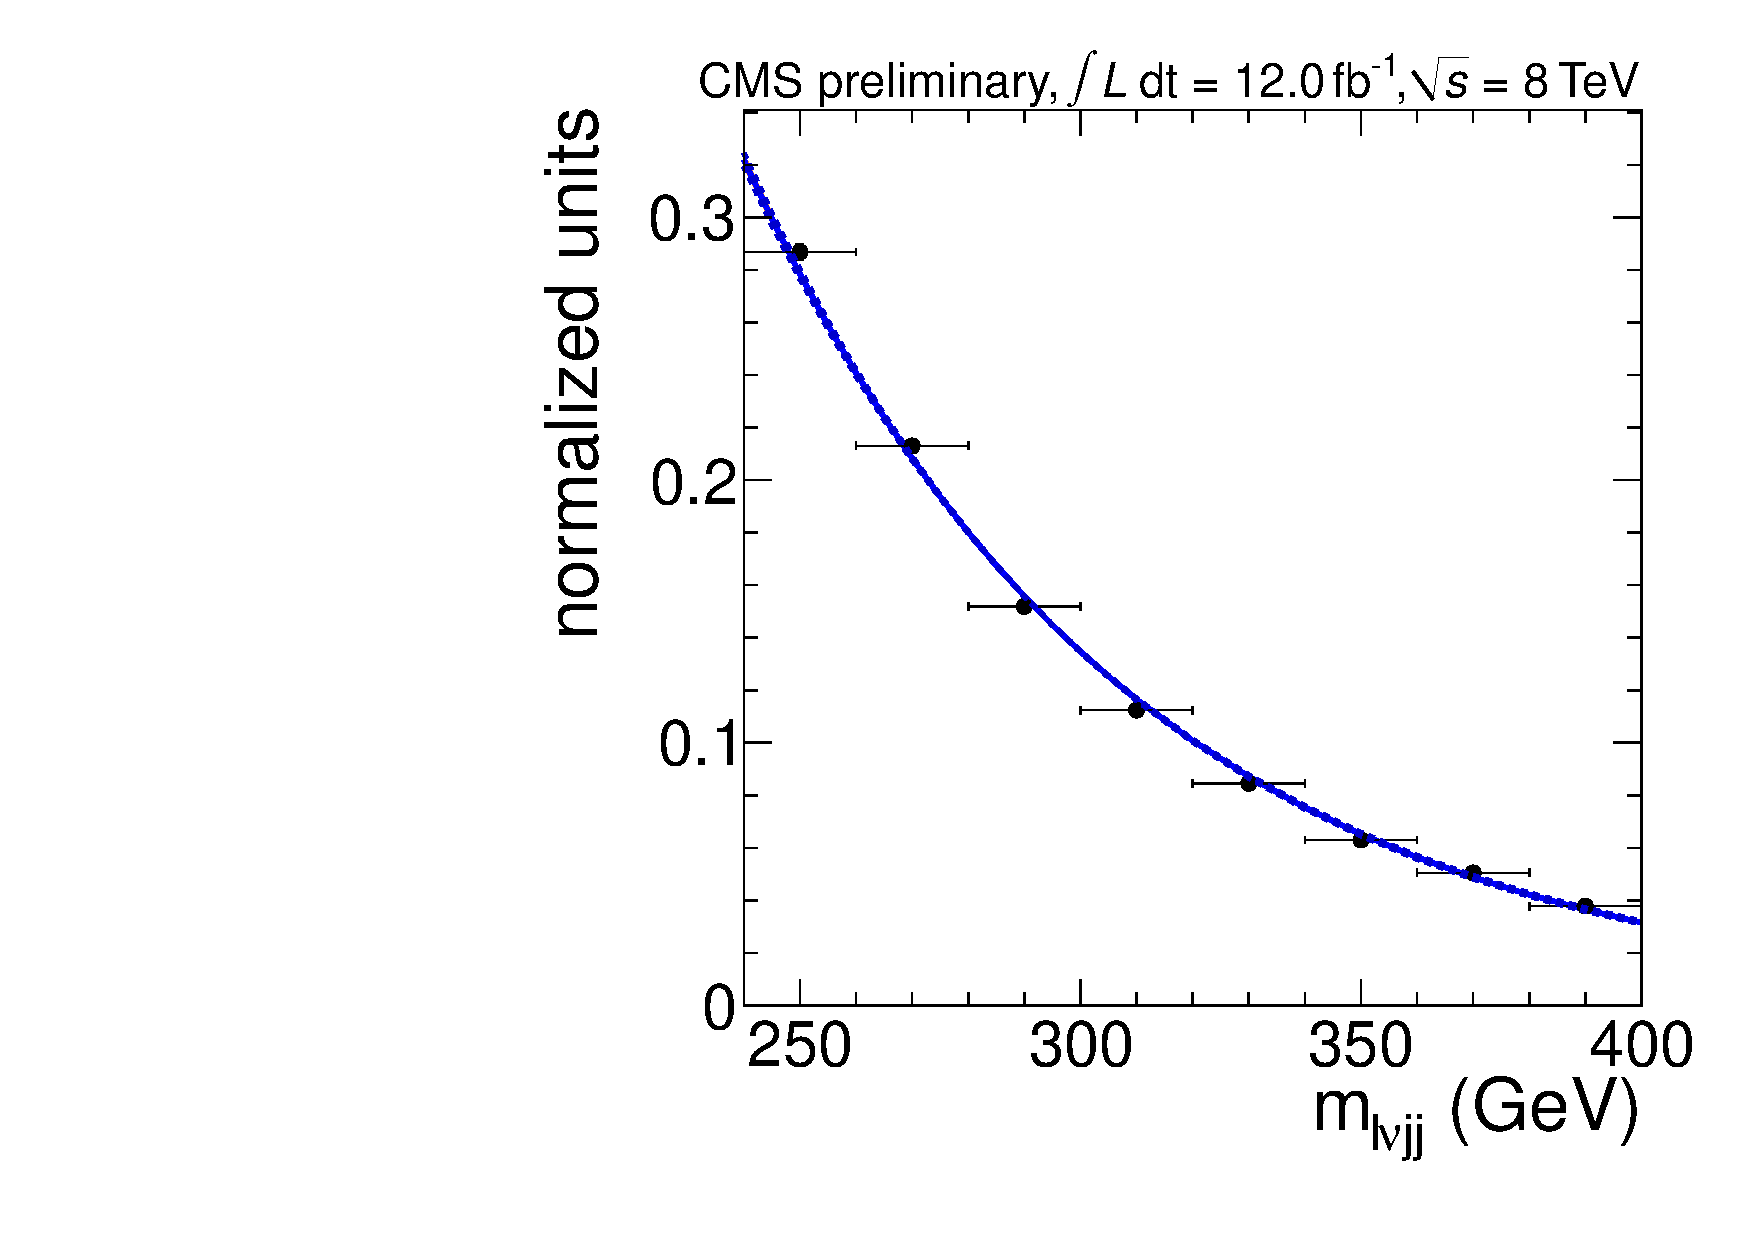
\includegraphics[width=0.45\textwidth]{plots/2012_WJetsShape/H300_Mlvjj_Muon_2jets_WpJShape.pdf}
    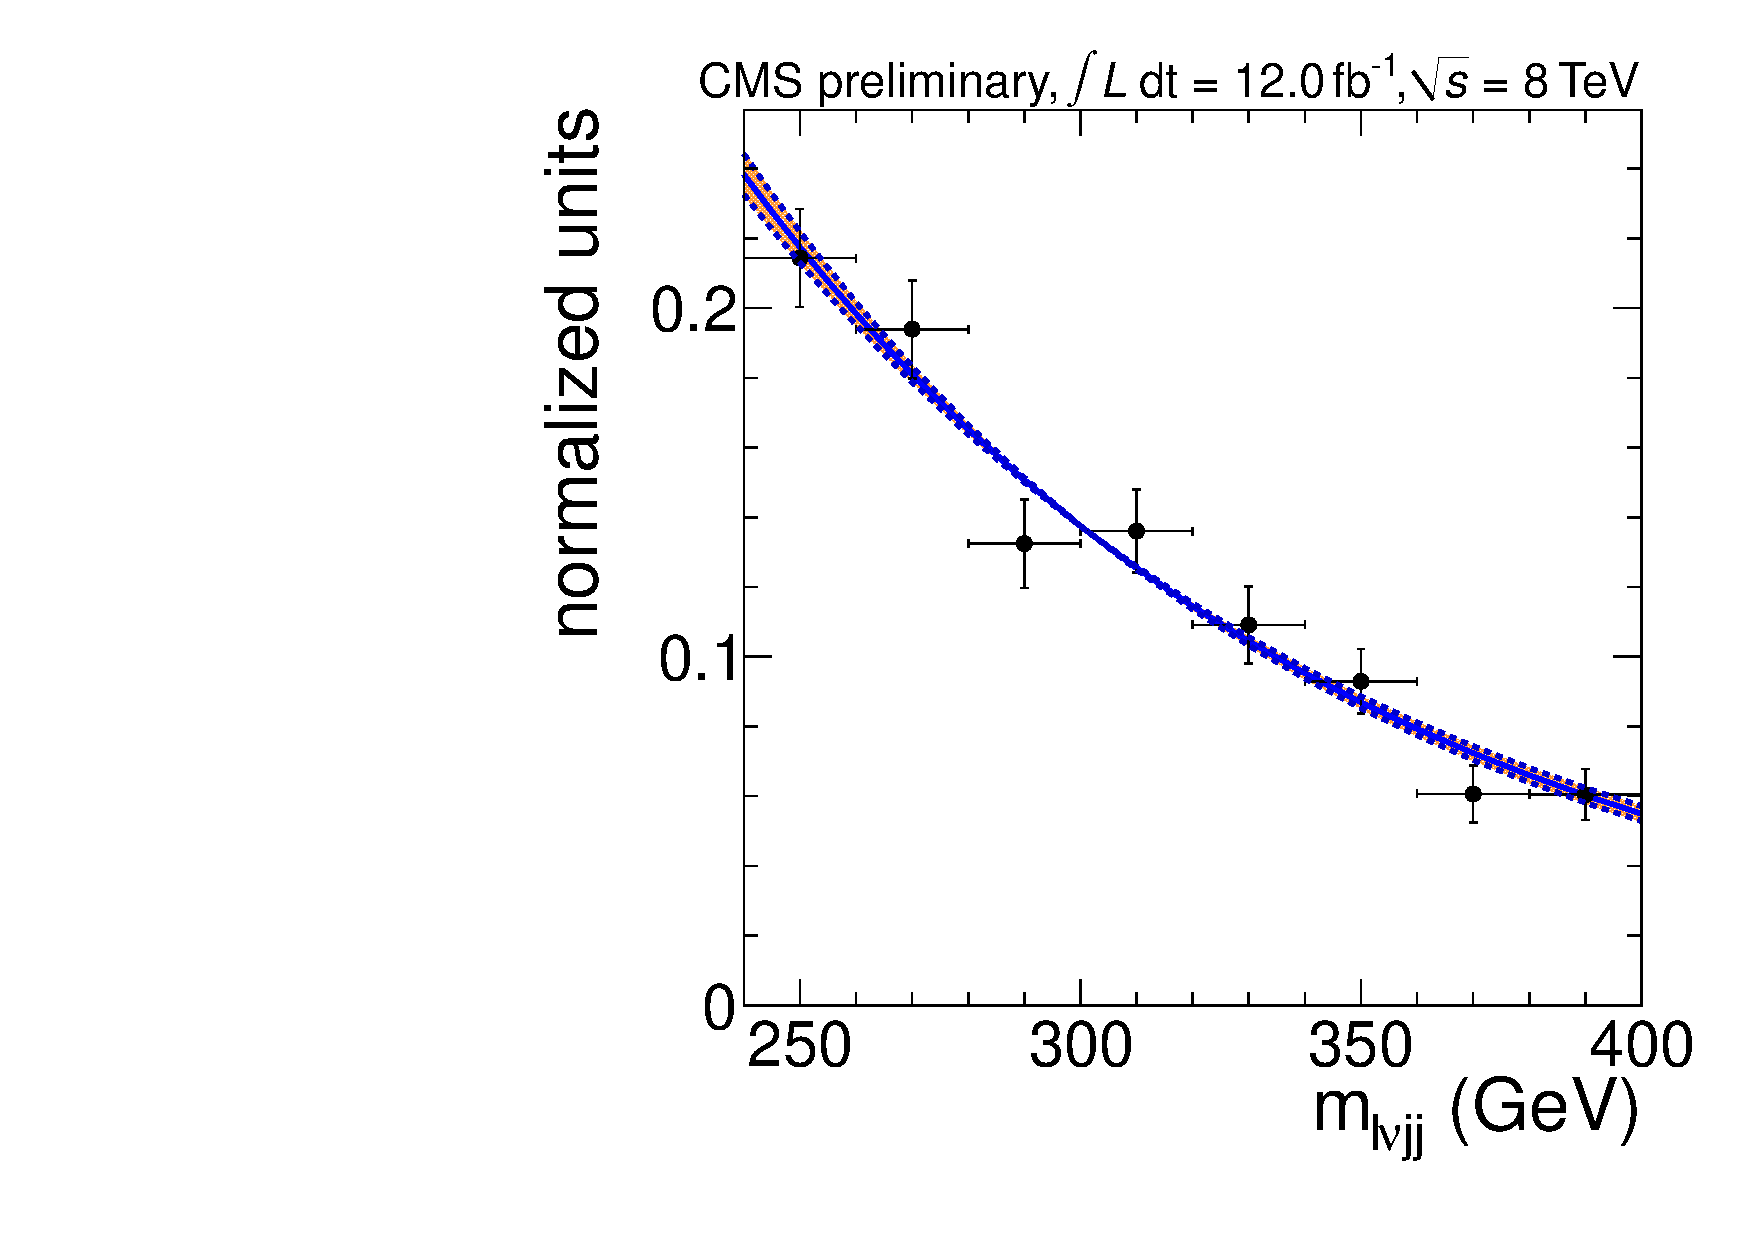
\includegraphics[width=0.45\textwidth]{plots/2012_WJetsShape/H300_Mlvjj_Muon_3jets_WpJShape.pdf}
    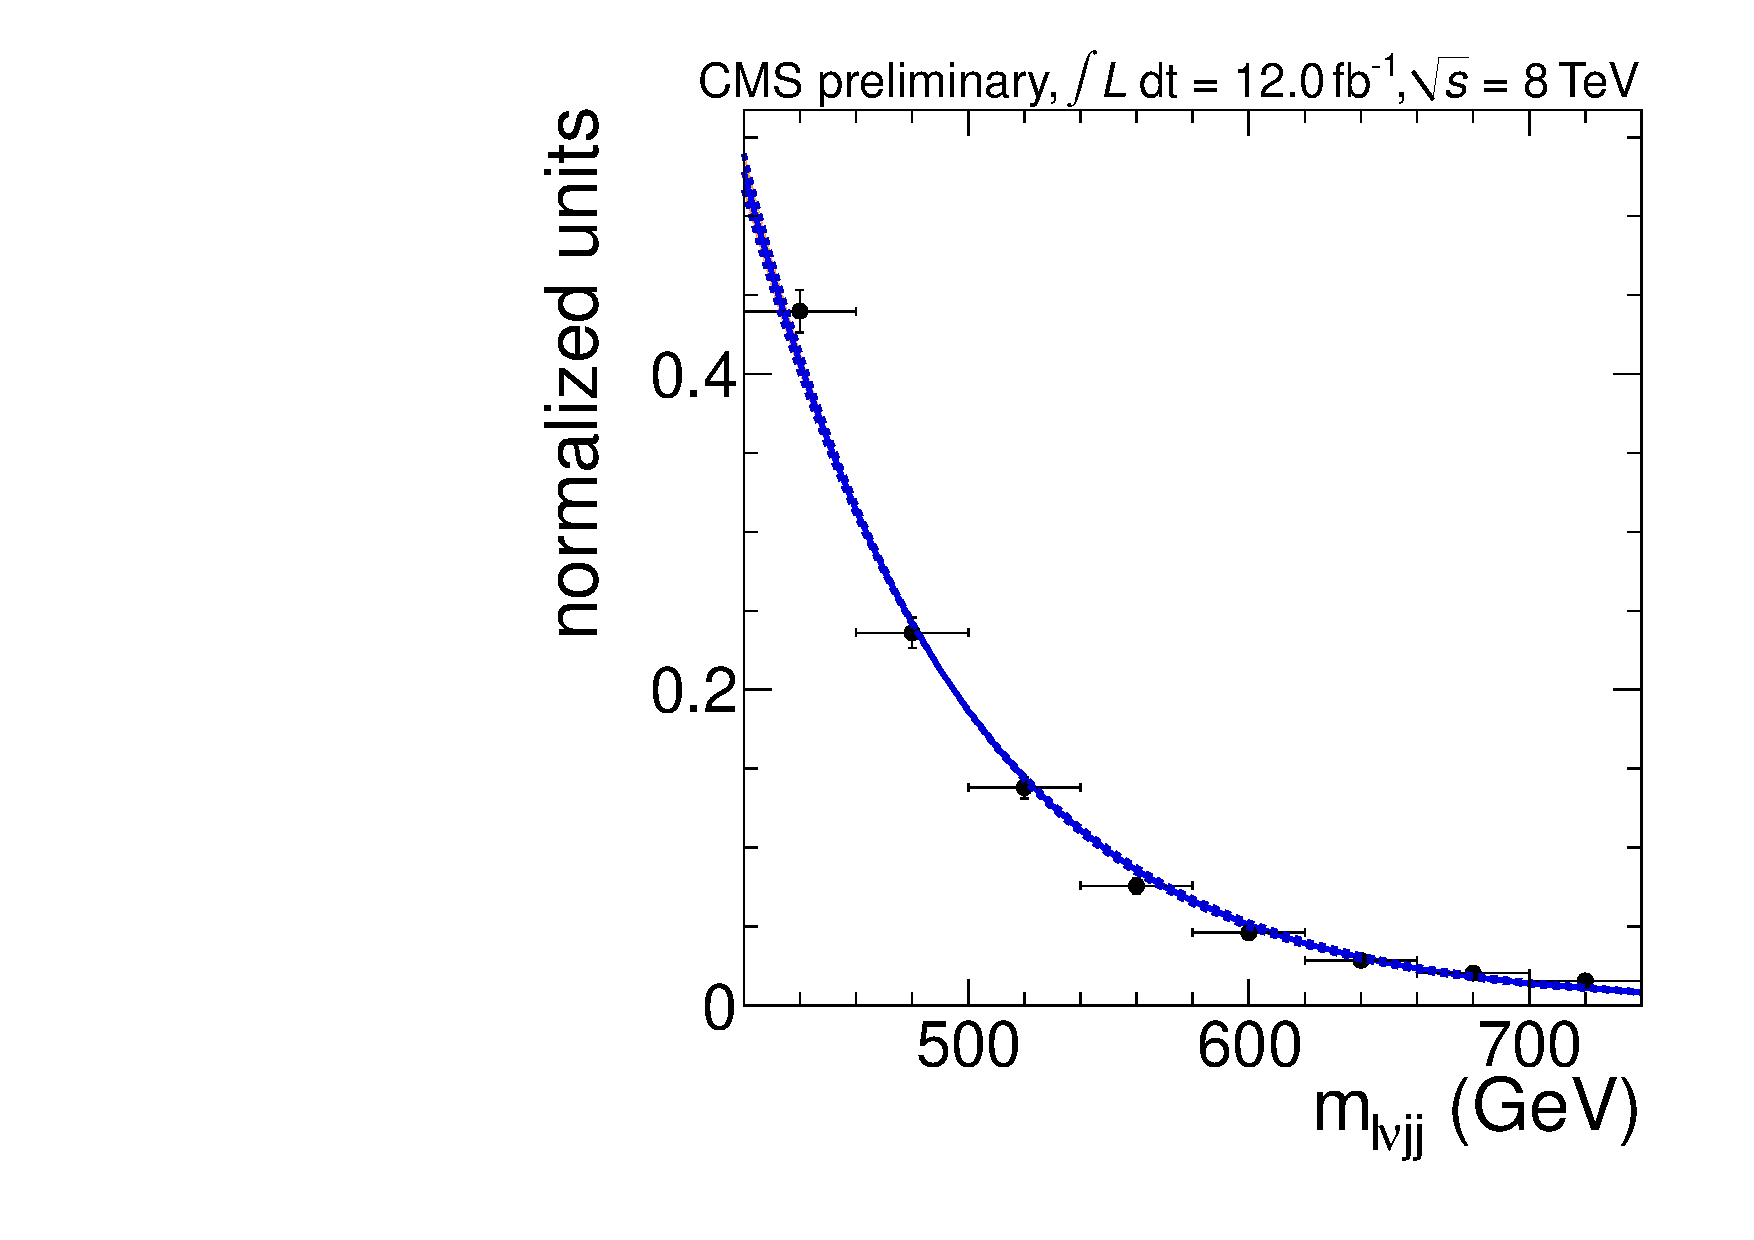
\includegraphics[width=0.45\textwidth]{plots/2012_WJetsShape/H500_Mlvjj_Muon_2jets_WpJShape.pdf}
    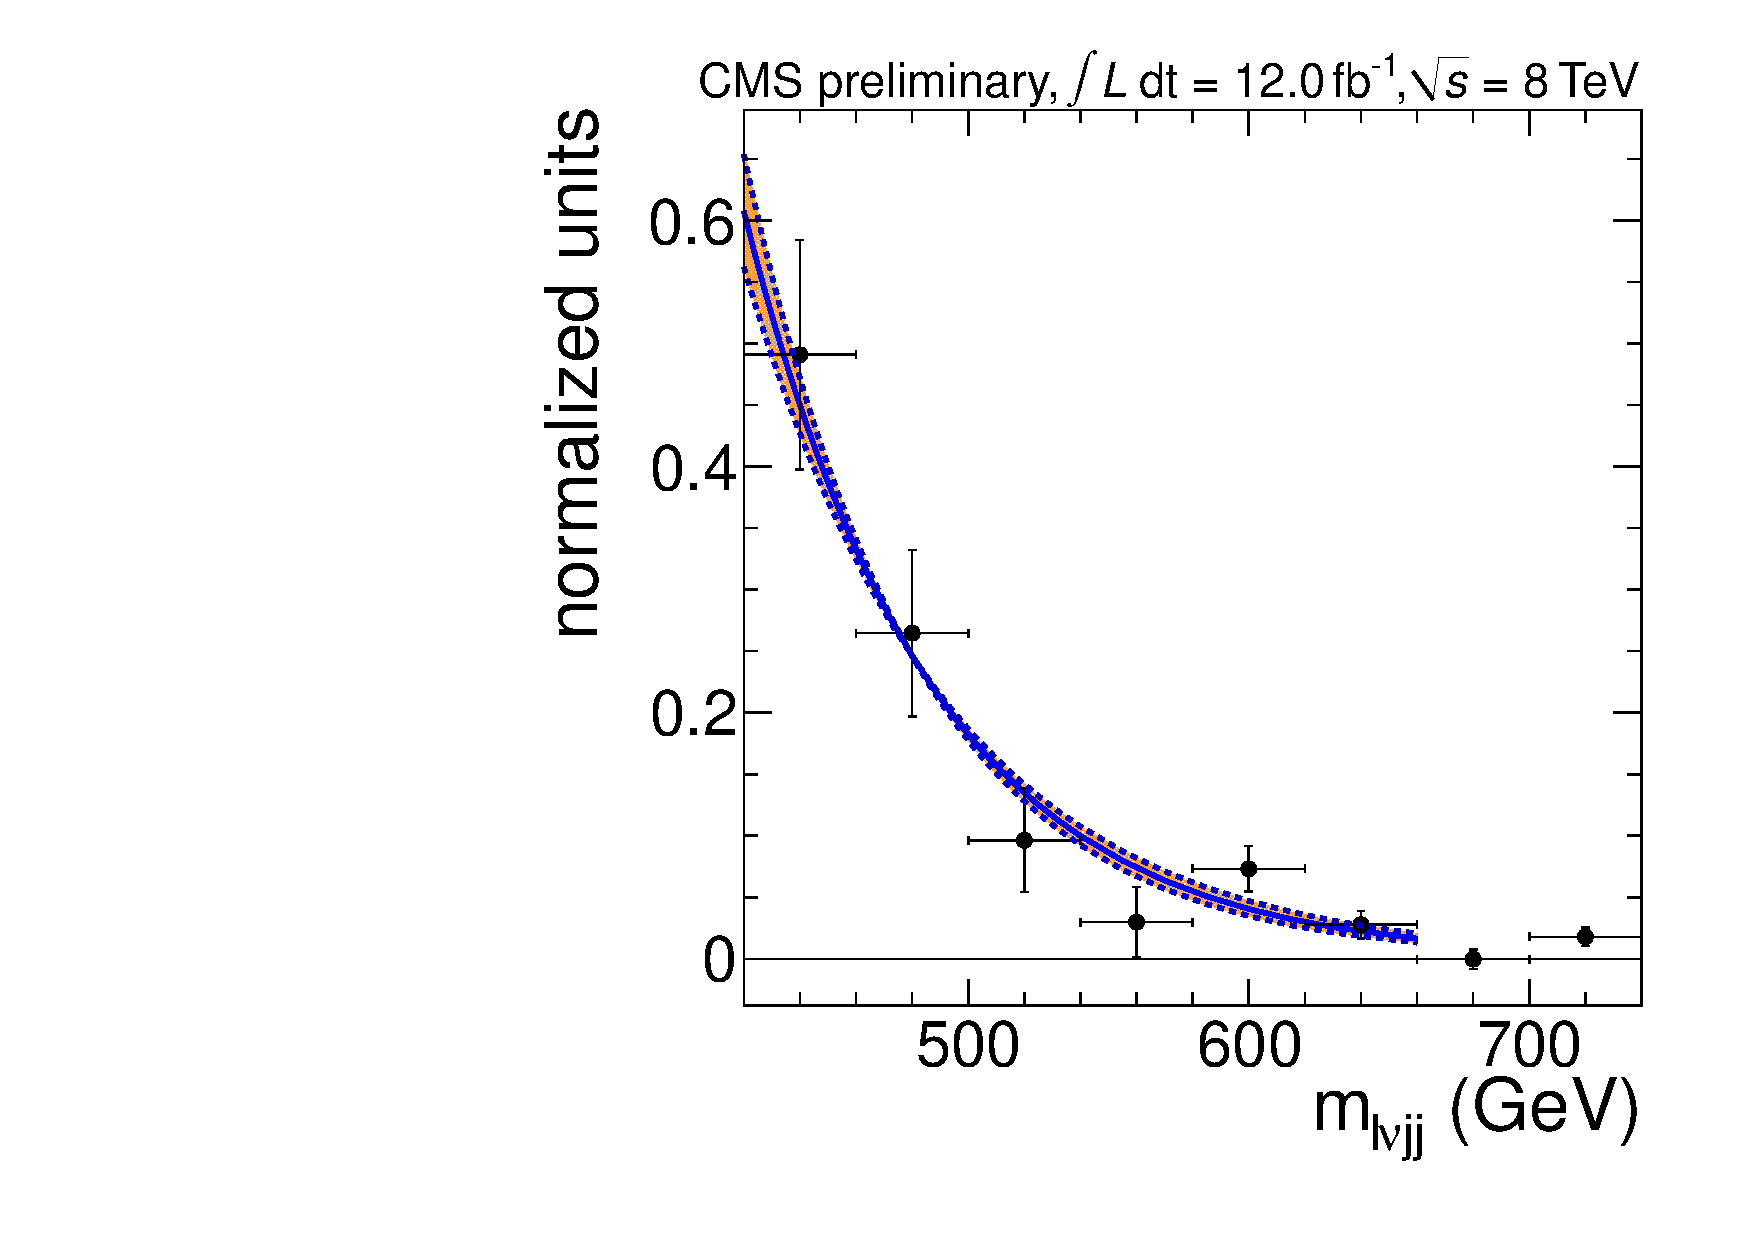
\includegraphics[width=0.45\textwidth]{plots/2012_WJetsShape/H500_Mlvjj_Muon_3jets_WpJShape.pdf}
    \caption{\label{fig:Wjets_dd_example} 
    The distribution of the extrapolated background in the signal region is reported for
    the Higgs mass hypotheses of 200~GeV (top row), 300~GeV (middle row) and 500~GeV (bottom
    row). The left and right columns display results for the muon 2jet and 3jet cases, respectively.
    The points represent the extrapolated points, while the blue line shows the fitting function and
    the blue dashed lines are the uncertainty on the shape.}
\end{figure}

The four-body mass distributions of background events in the signal regions,
derived from the $m_{jj}$ data sidebands, are shown in Figures~\ref{fig:m4_dd_example200}-\ref{fig:m4_dd_example500}.
%%The data in the signal region is blinded/not shown.

\begin{figure}[!t]
  \centering
%%  \subfigure[electron 2 jets, 190 GeV Higgs]{
%%    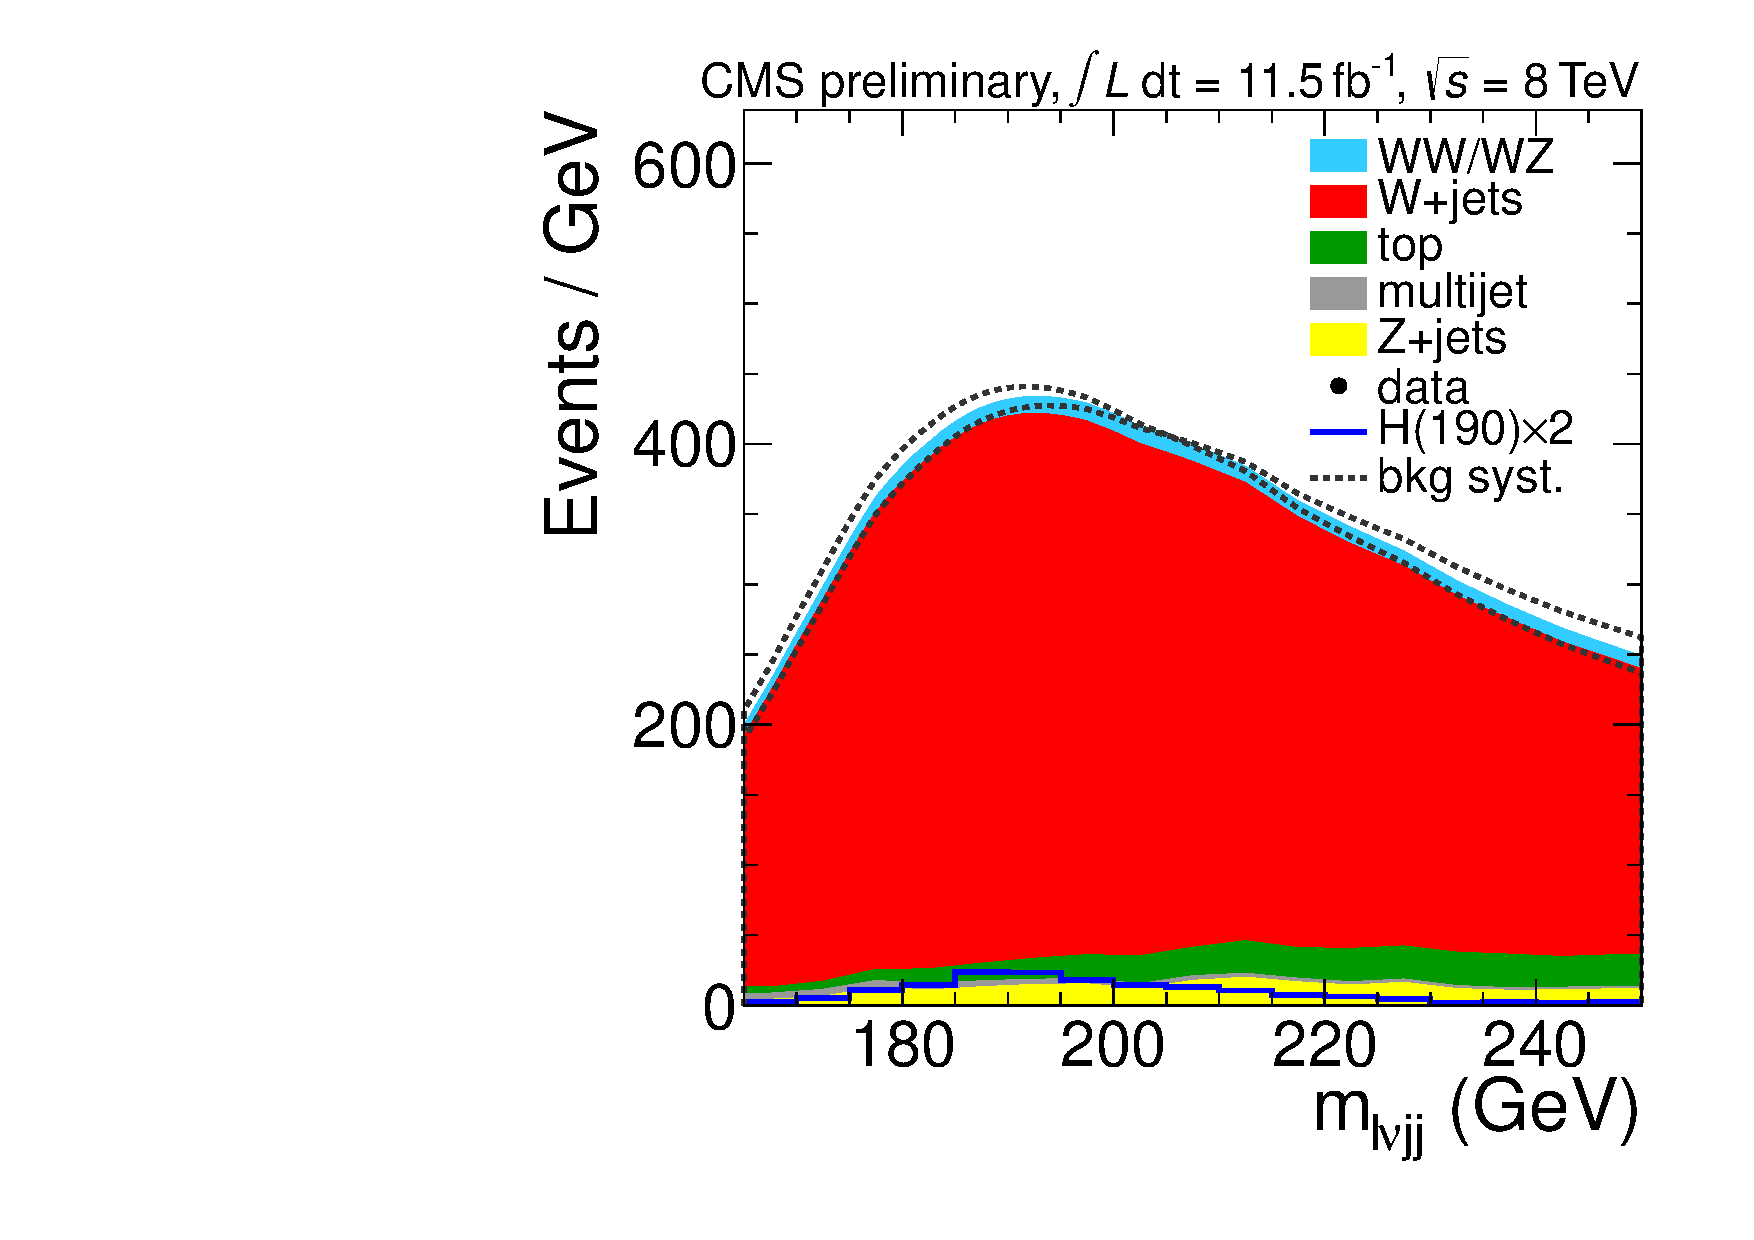
\includegraphics[width=0.45\textwidth]{plots/2012_FOURBSHAPES/H190_Mlvjj_Electron_2jets_Stacked}
%%    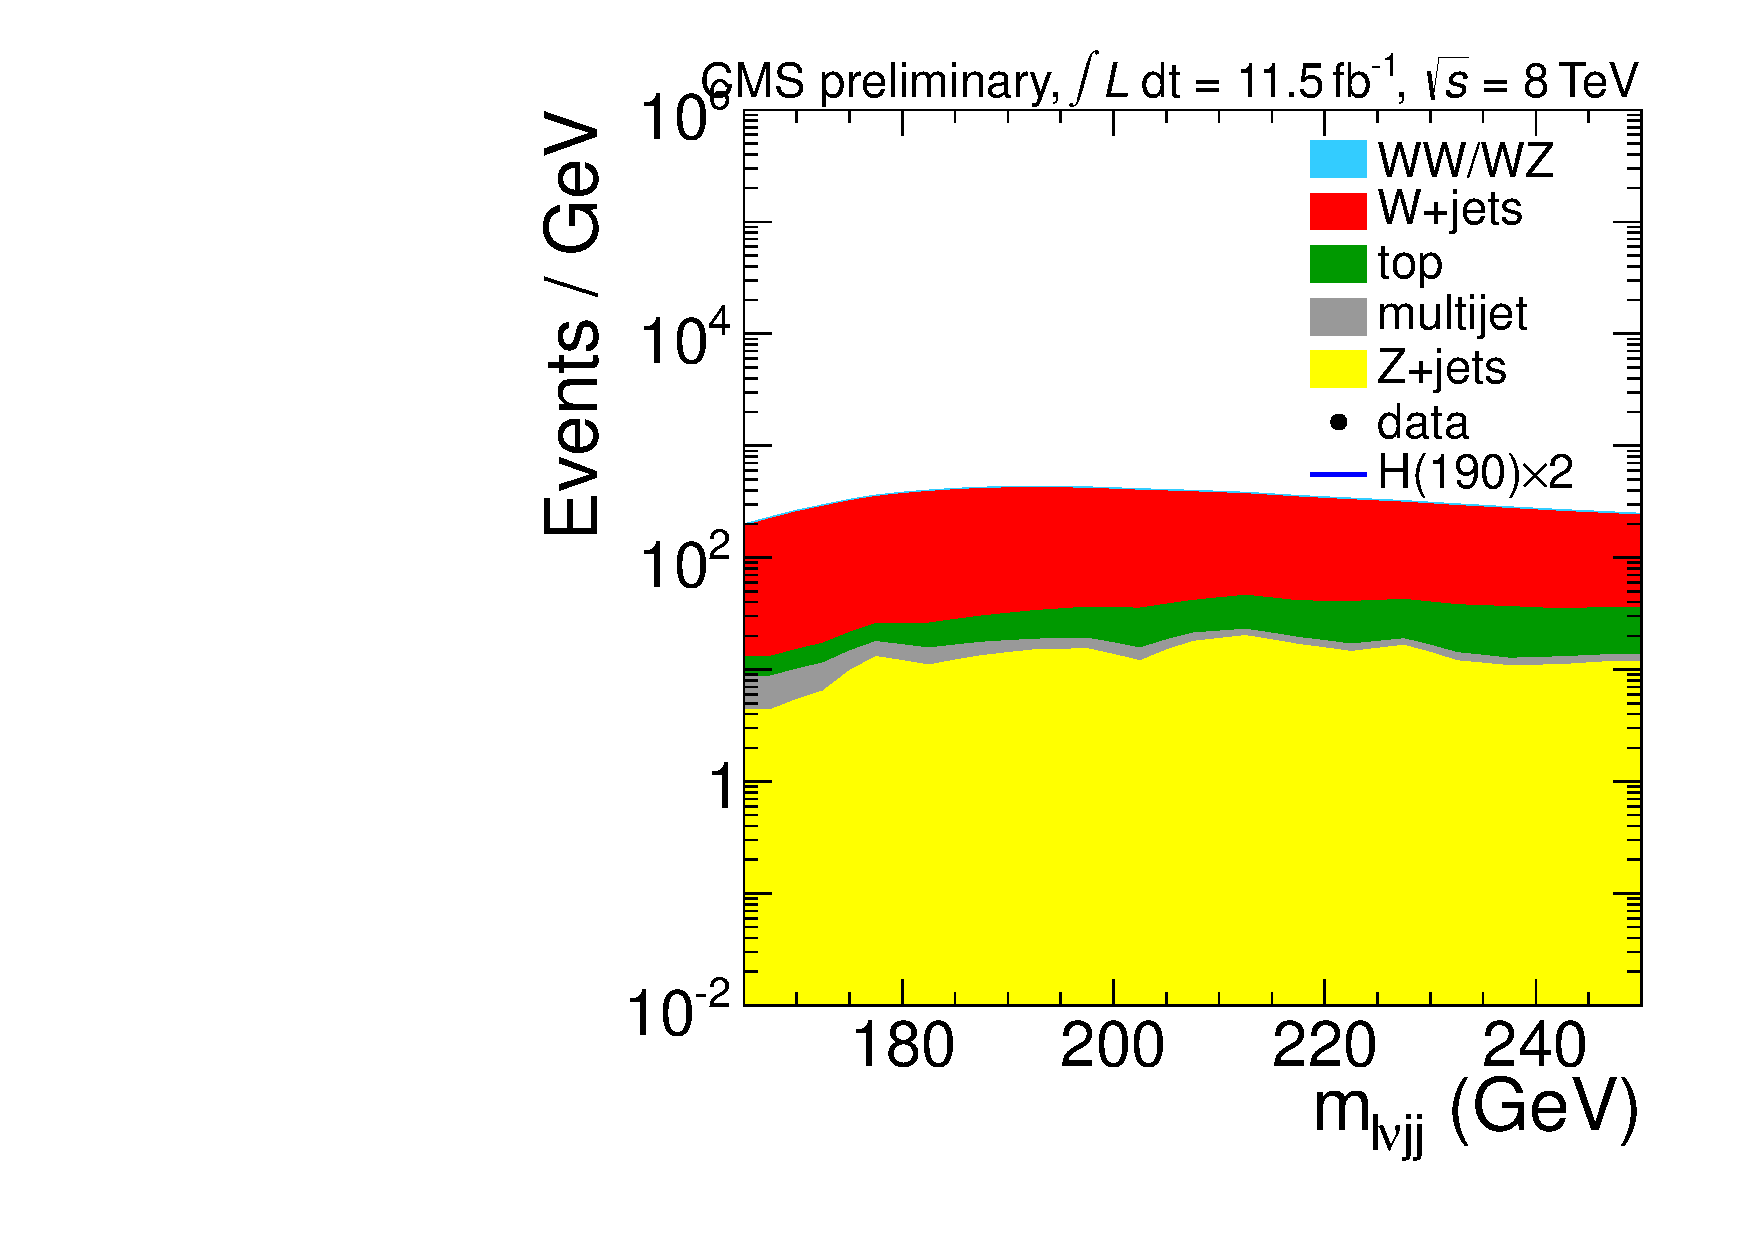
\includegraphics[width=0.45\textwidth]{plots/2012_FOURBSHAPES/H190_Mlvjj_Electron_2jets_Stacked_log}
  \subfigure[electron 2 jets, 200 GeV Higgs]{
      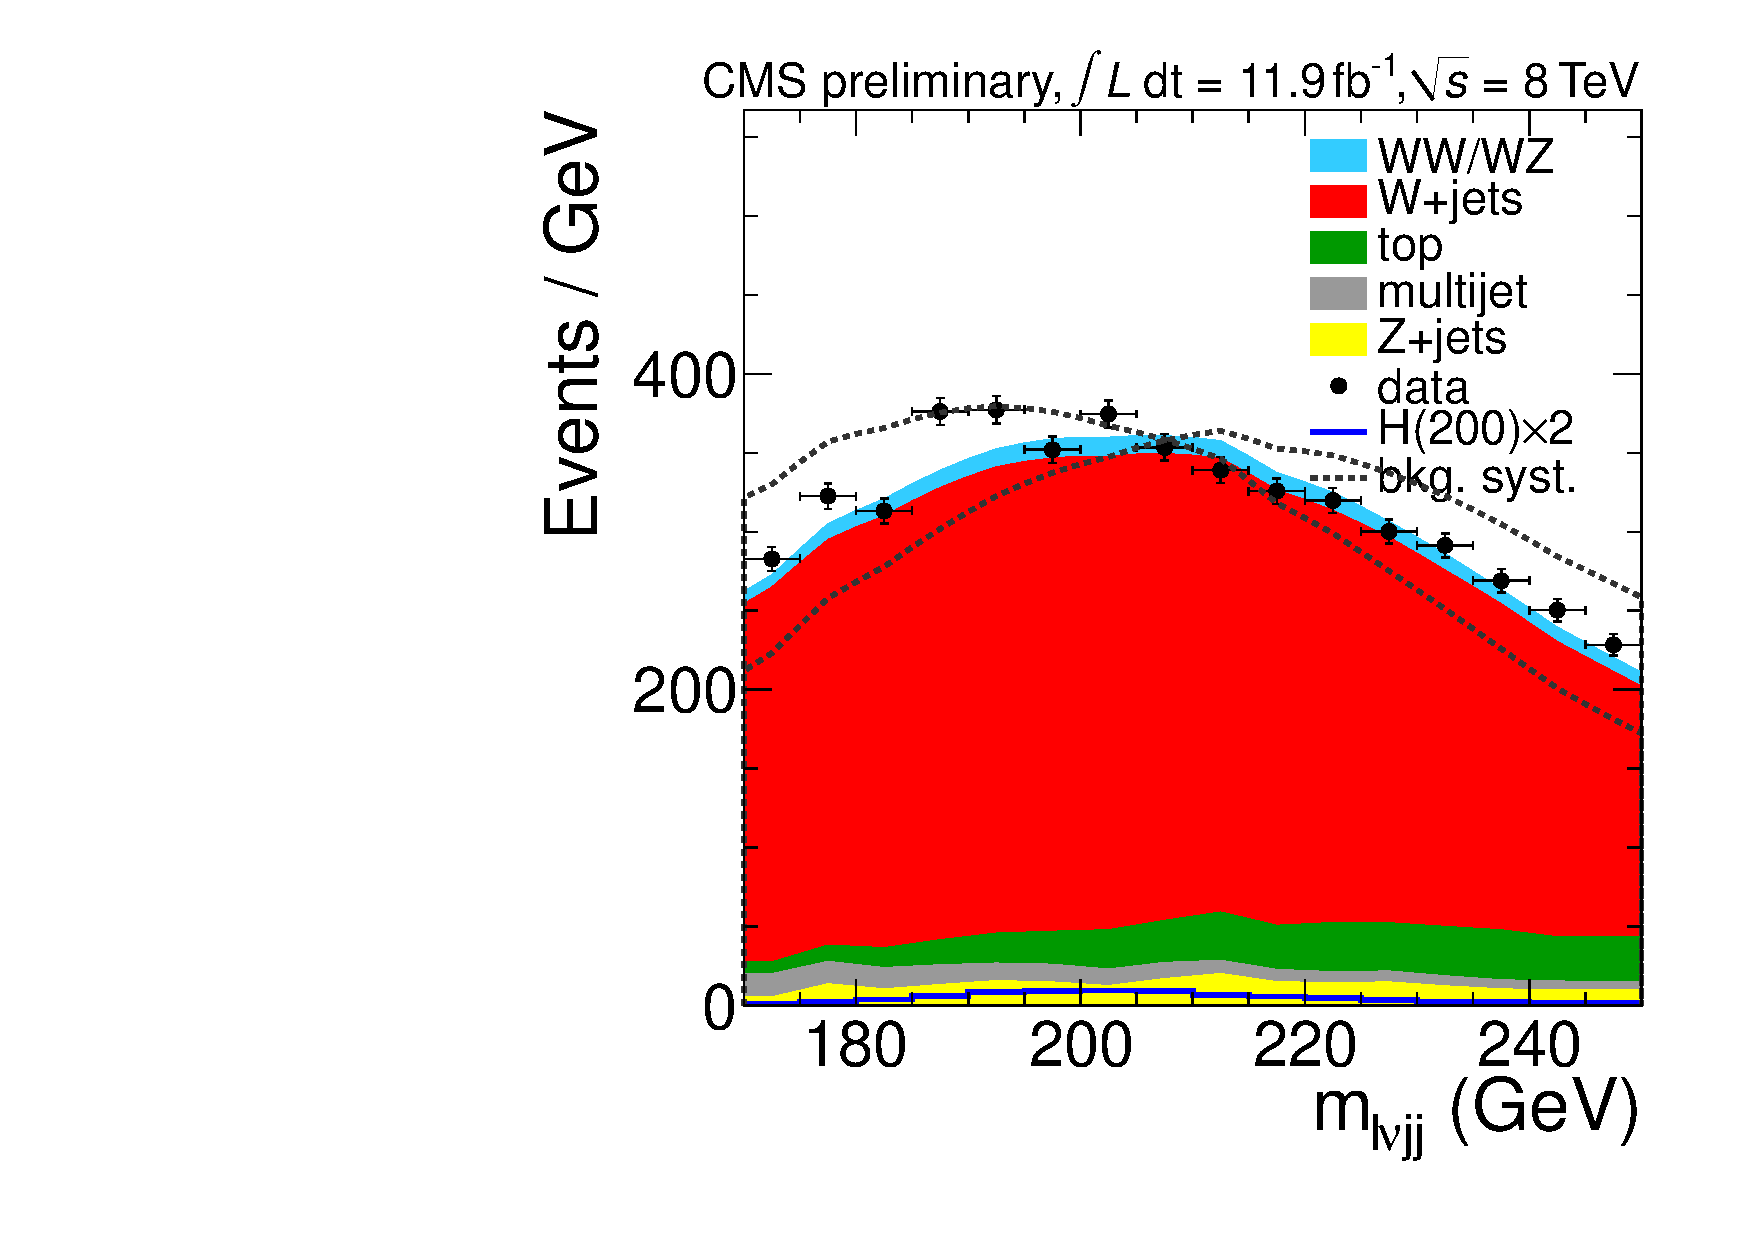
\includegraphics[width=0.45\textwidth]{plots/2012_FOURBSHAPES/H200_Mlvjj_Electron_2jets_Stacked}
      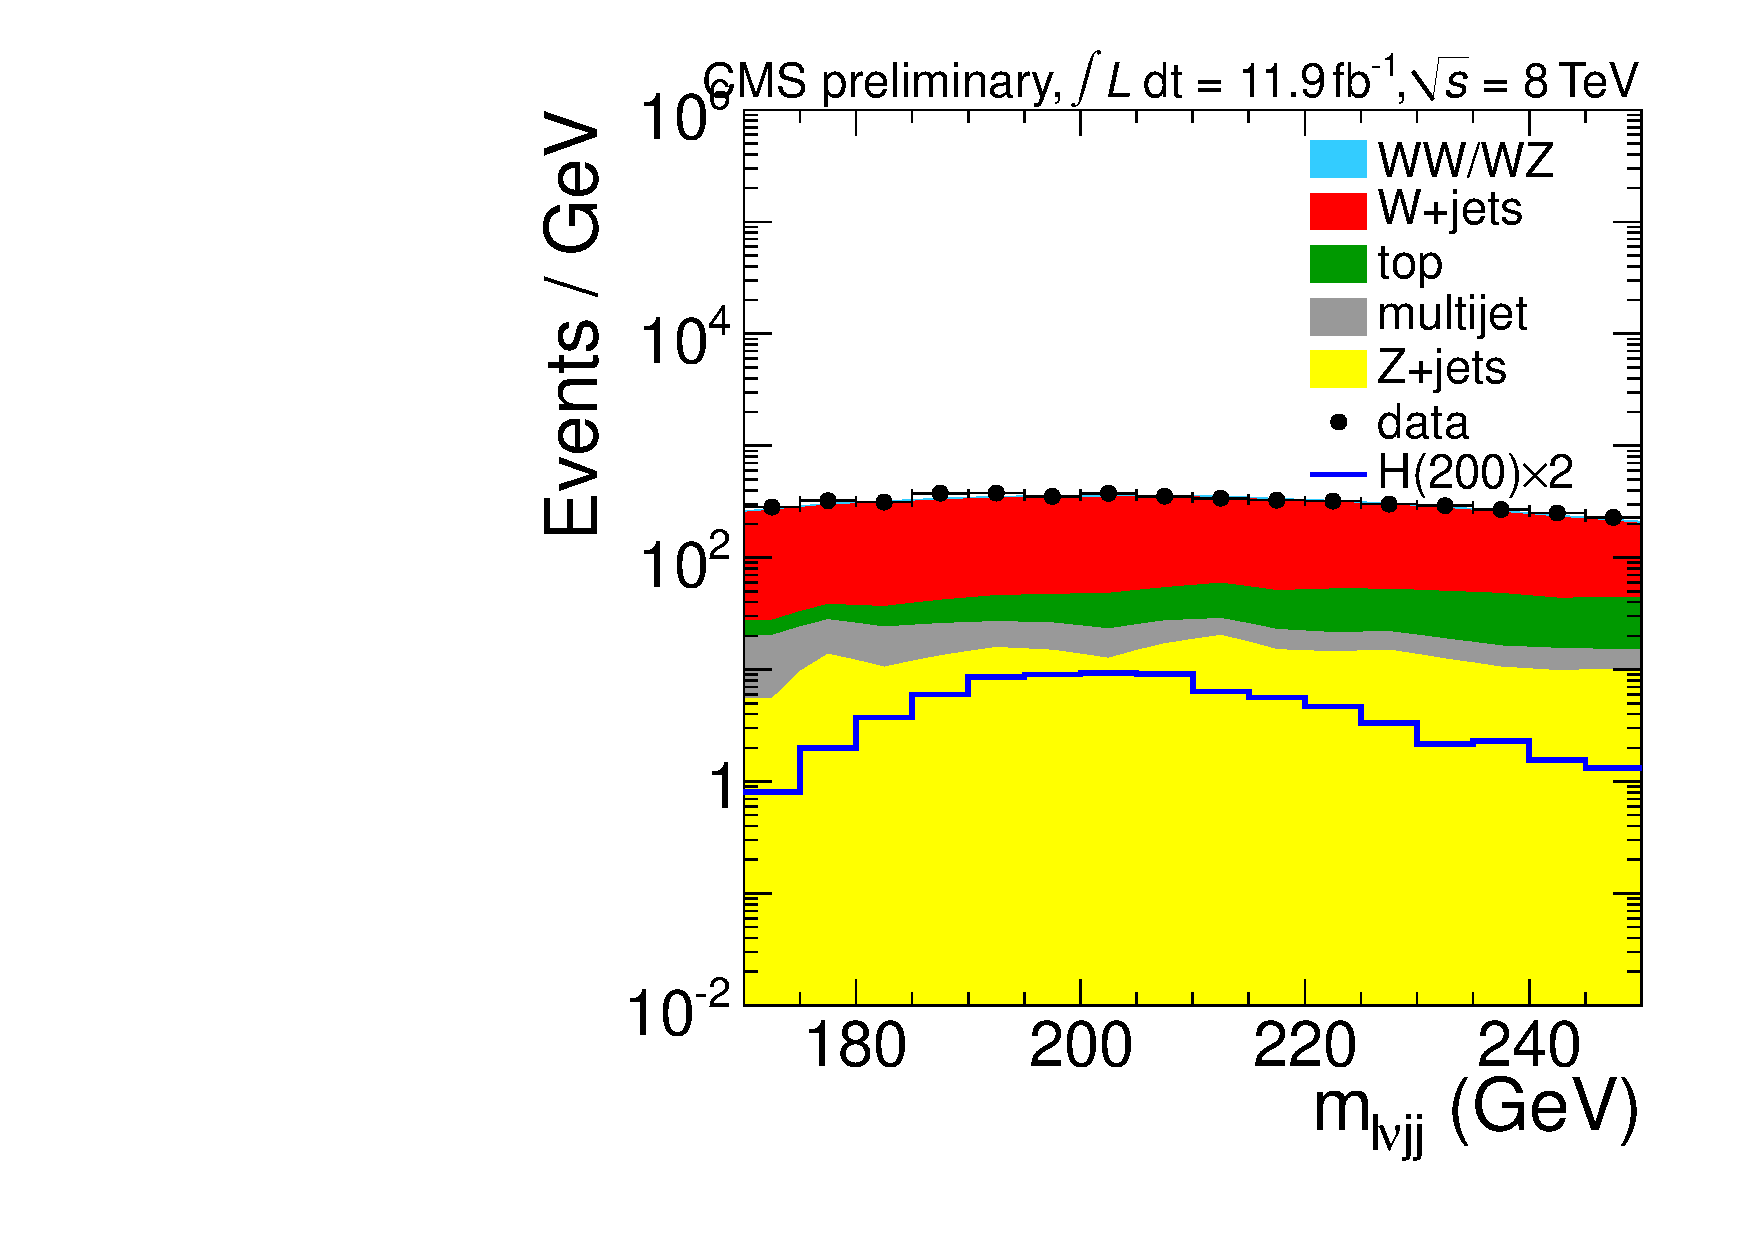
\includegraphics[width=0.45\textwidth]{plots/2012_FOURBSHAPES/H200_Mlvjj_Electron_2jets_Stacked_log}
%%      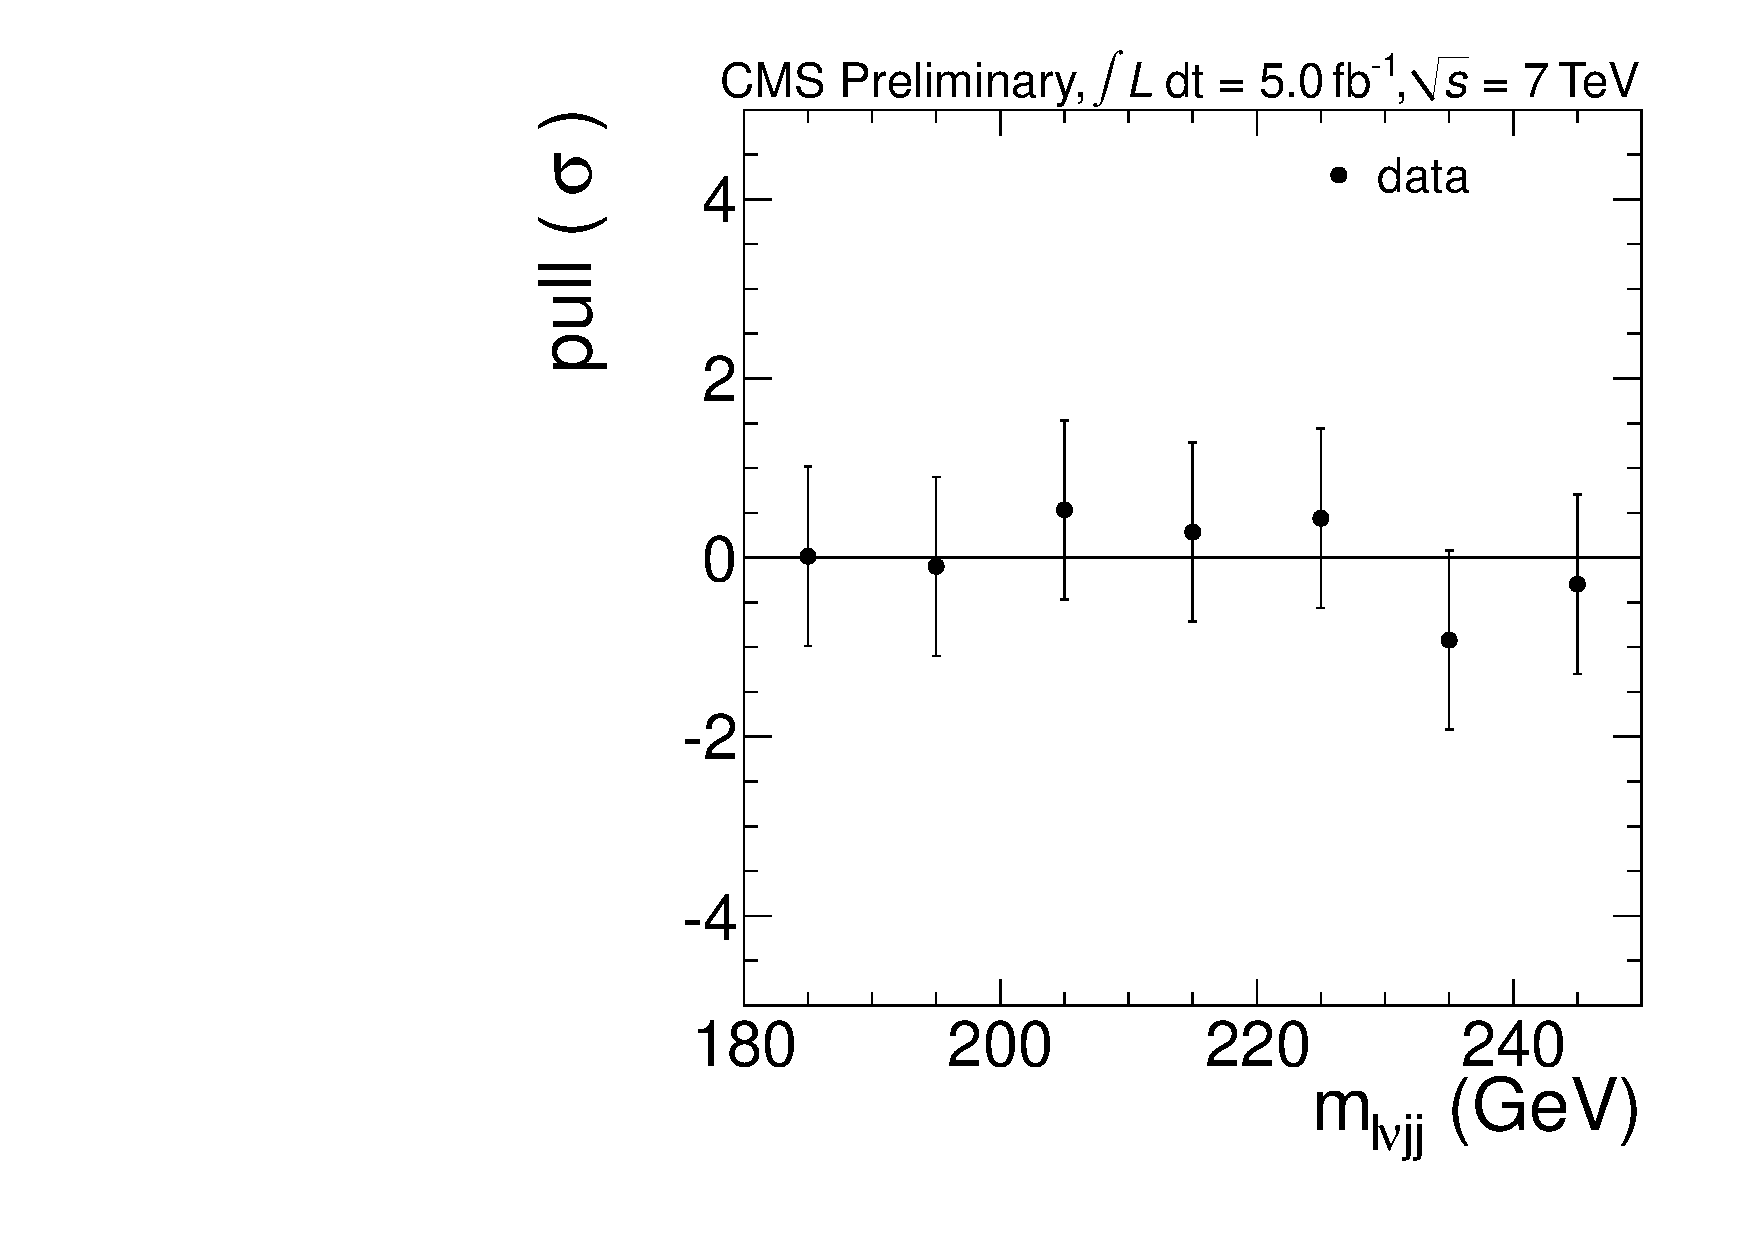
\includegraphics[width=0.3\textwidth]{plots/2012_FOURBSHAPES/H200_Mlvjj_Electron_2jets_Pull}
}

%%\subfigure[electron 3 jets, 190 GeV Higgs]{
%%      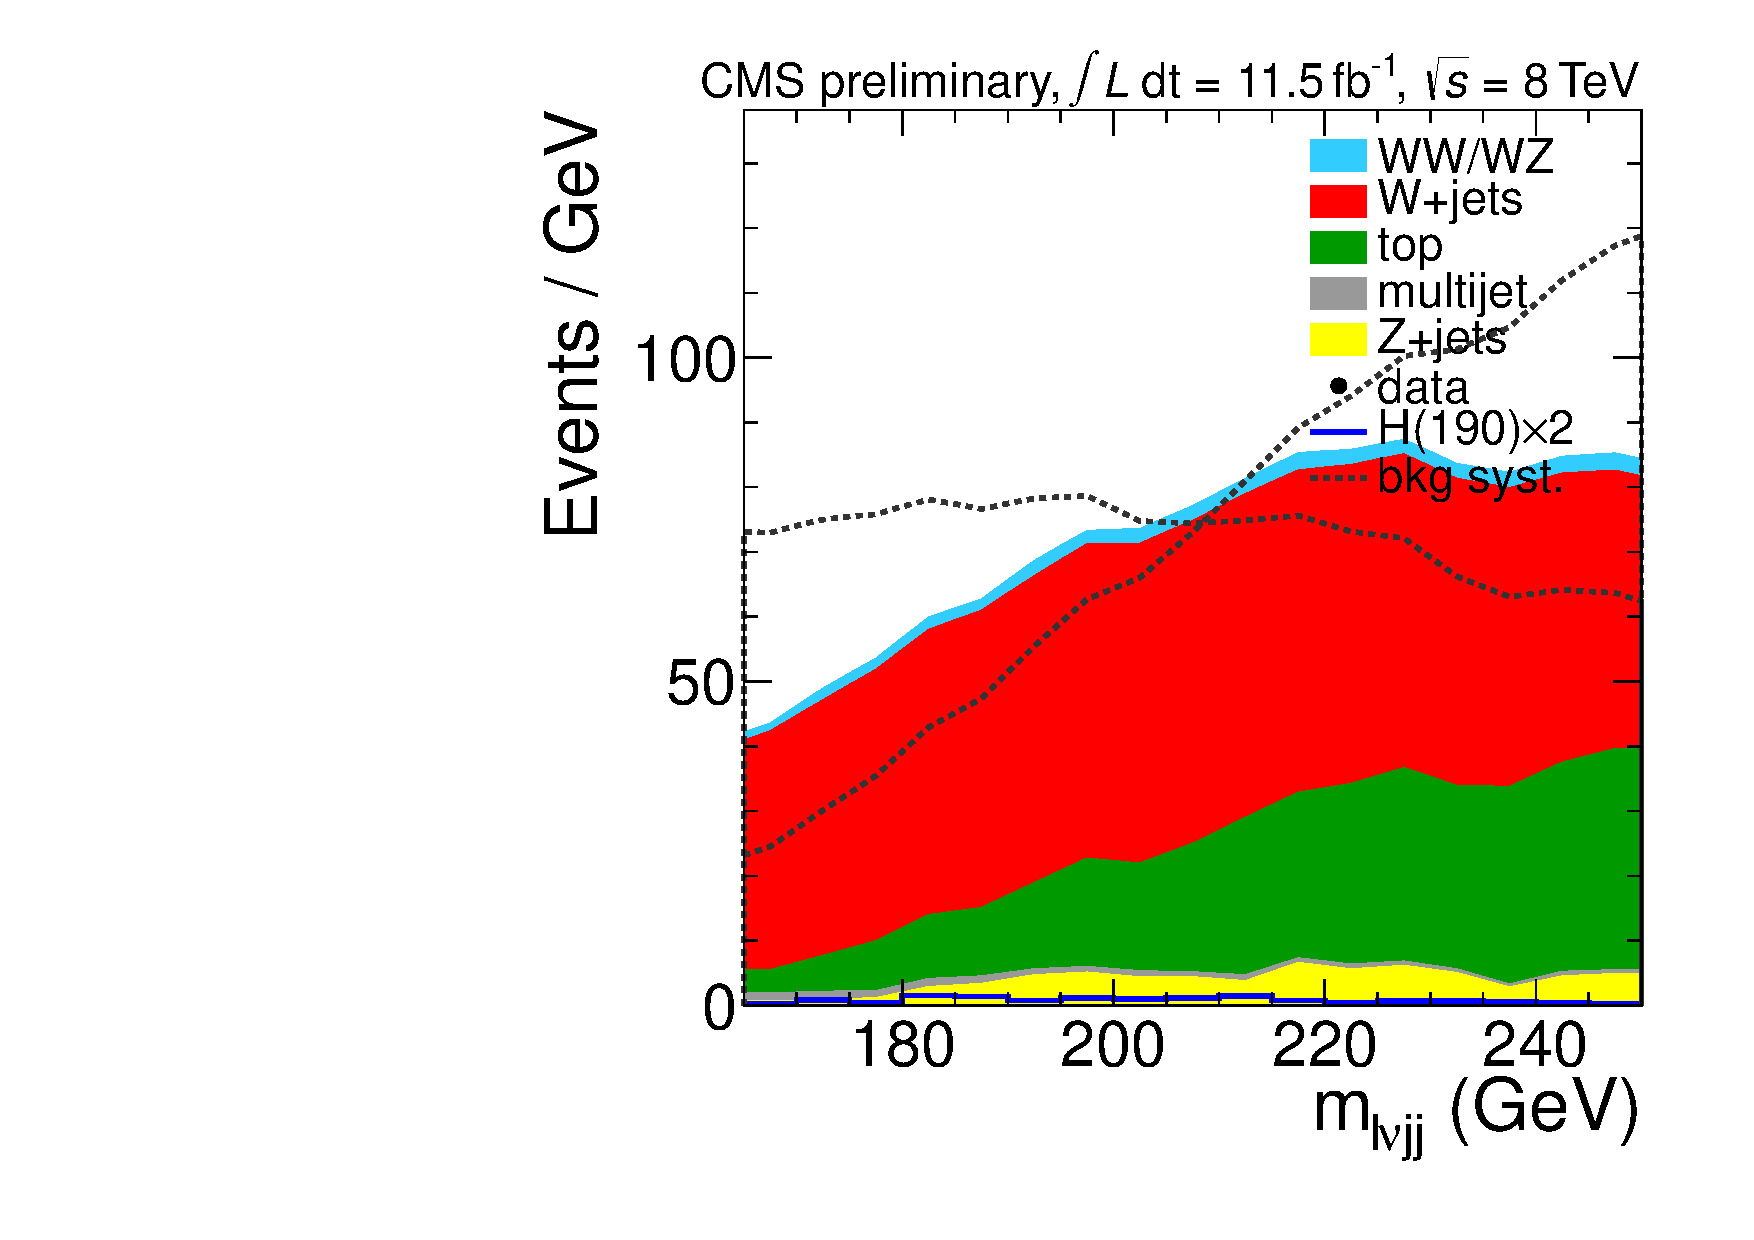
\includegraphics[width=0.45\textwidth]{plots/2012_FOURBSHAPES/H190_Mlvjj_Electron_3jets_Stacked}
%%      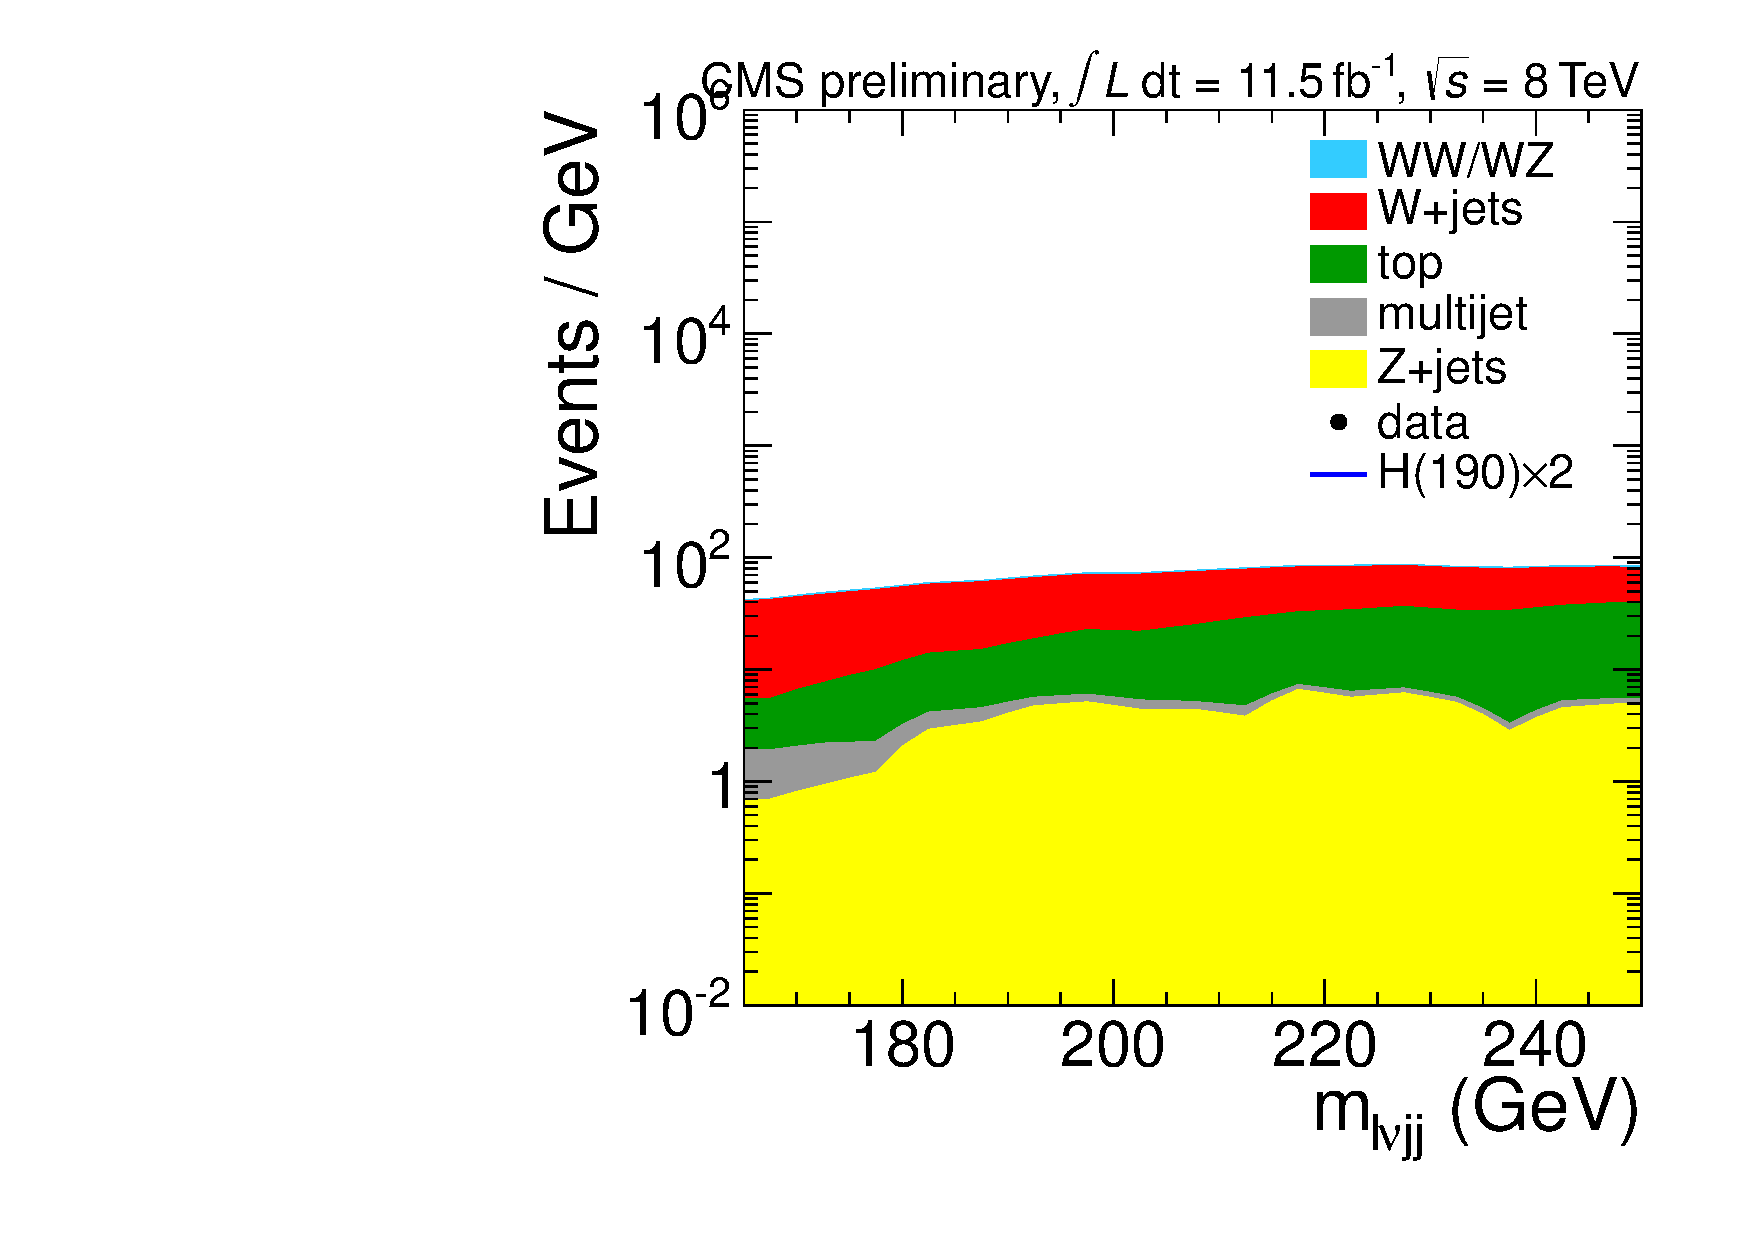
\includegraphics[width=0.45\textwidth]{plots/2012_FOURBSHAPES/H190_Mlvjj_Electron_3jets_Stacked_log}
\subfigure[electron 3 jets, 200 GeV Higgs]{
      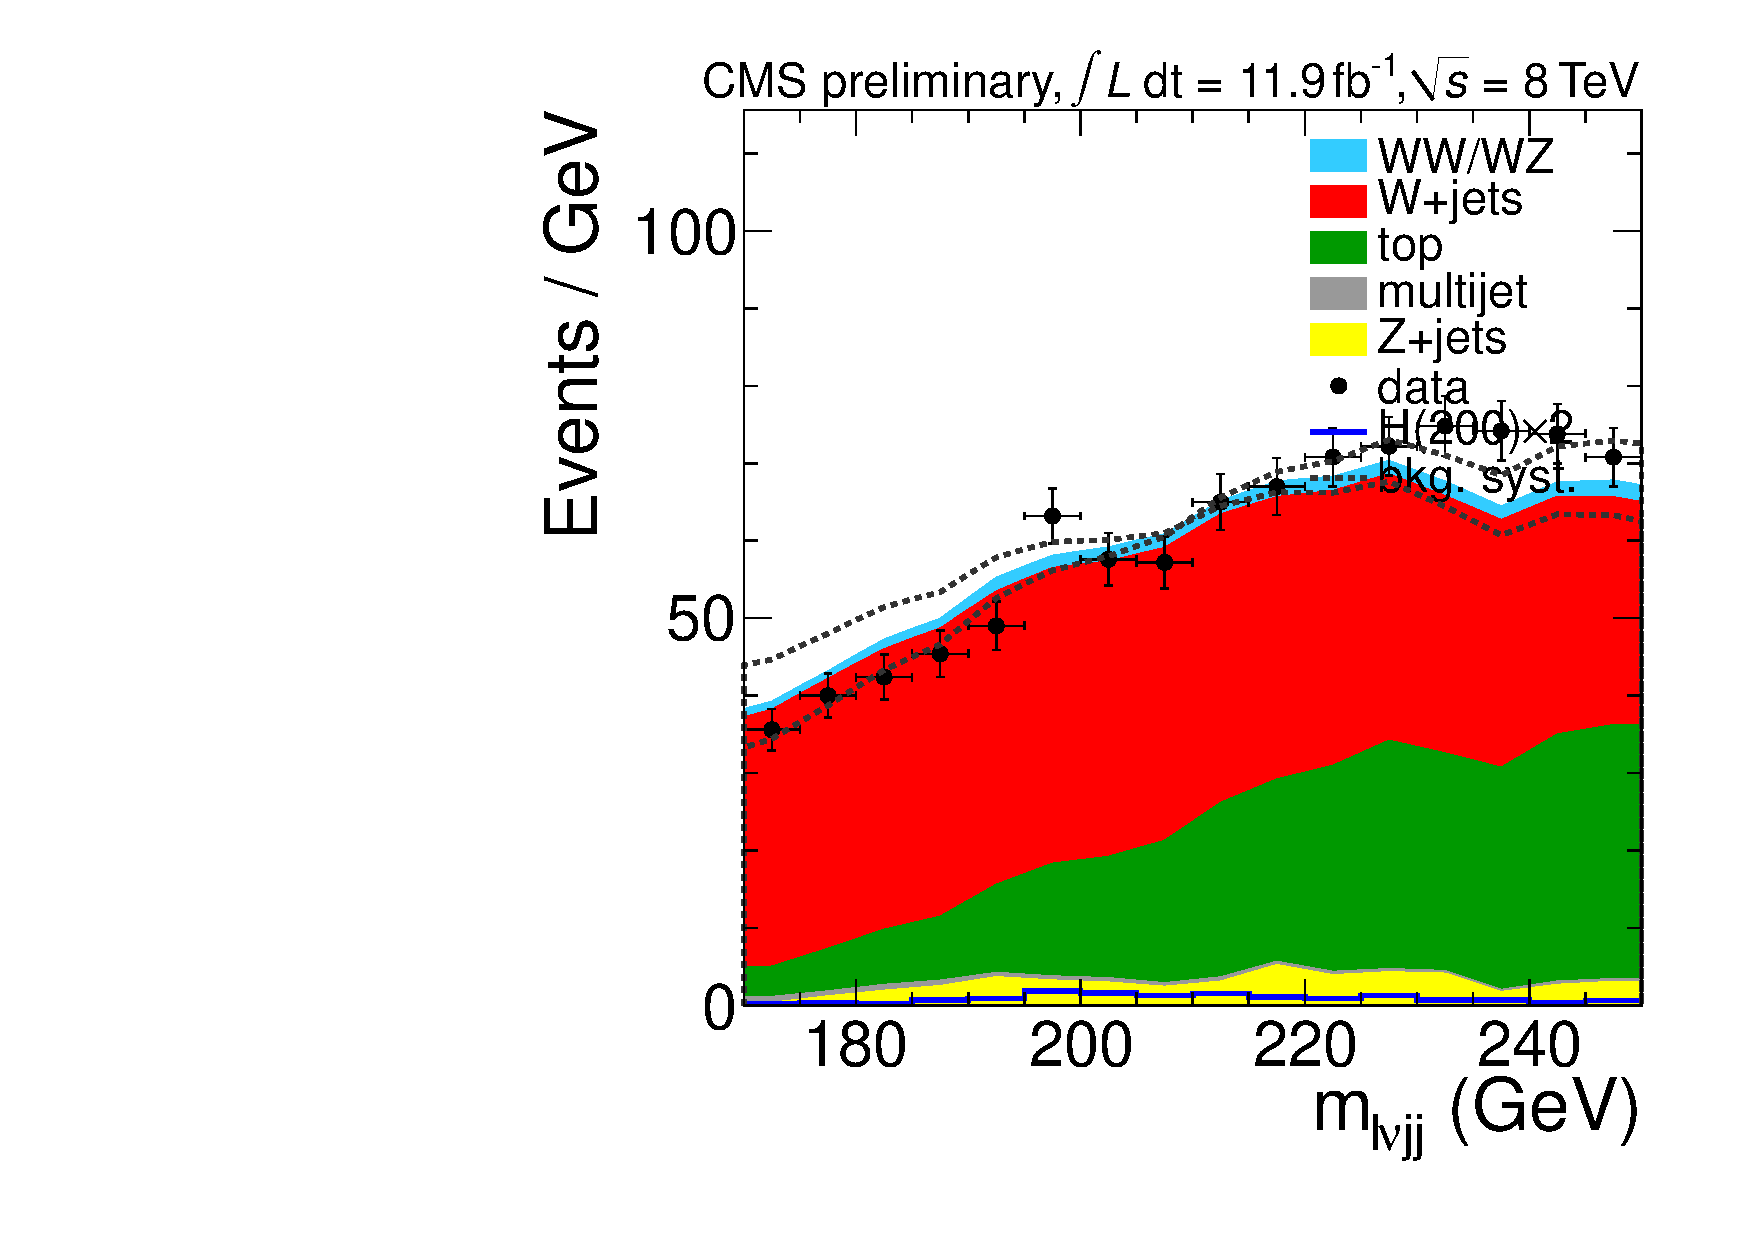
\includegraphics[width=0.45\textwidth]{plots/2012_FOURBSHAPES/H200_Mlvjj_Electron_3jets_Stacked}
      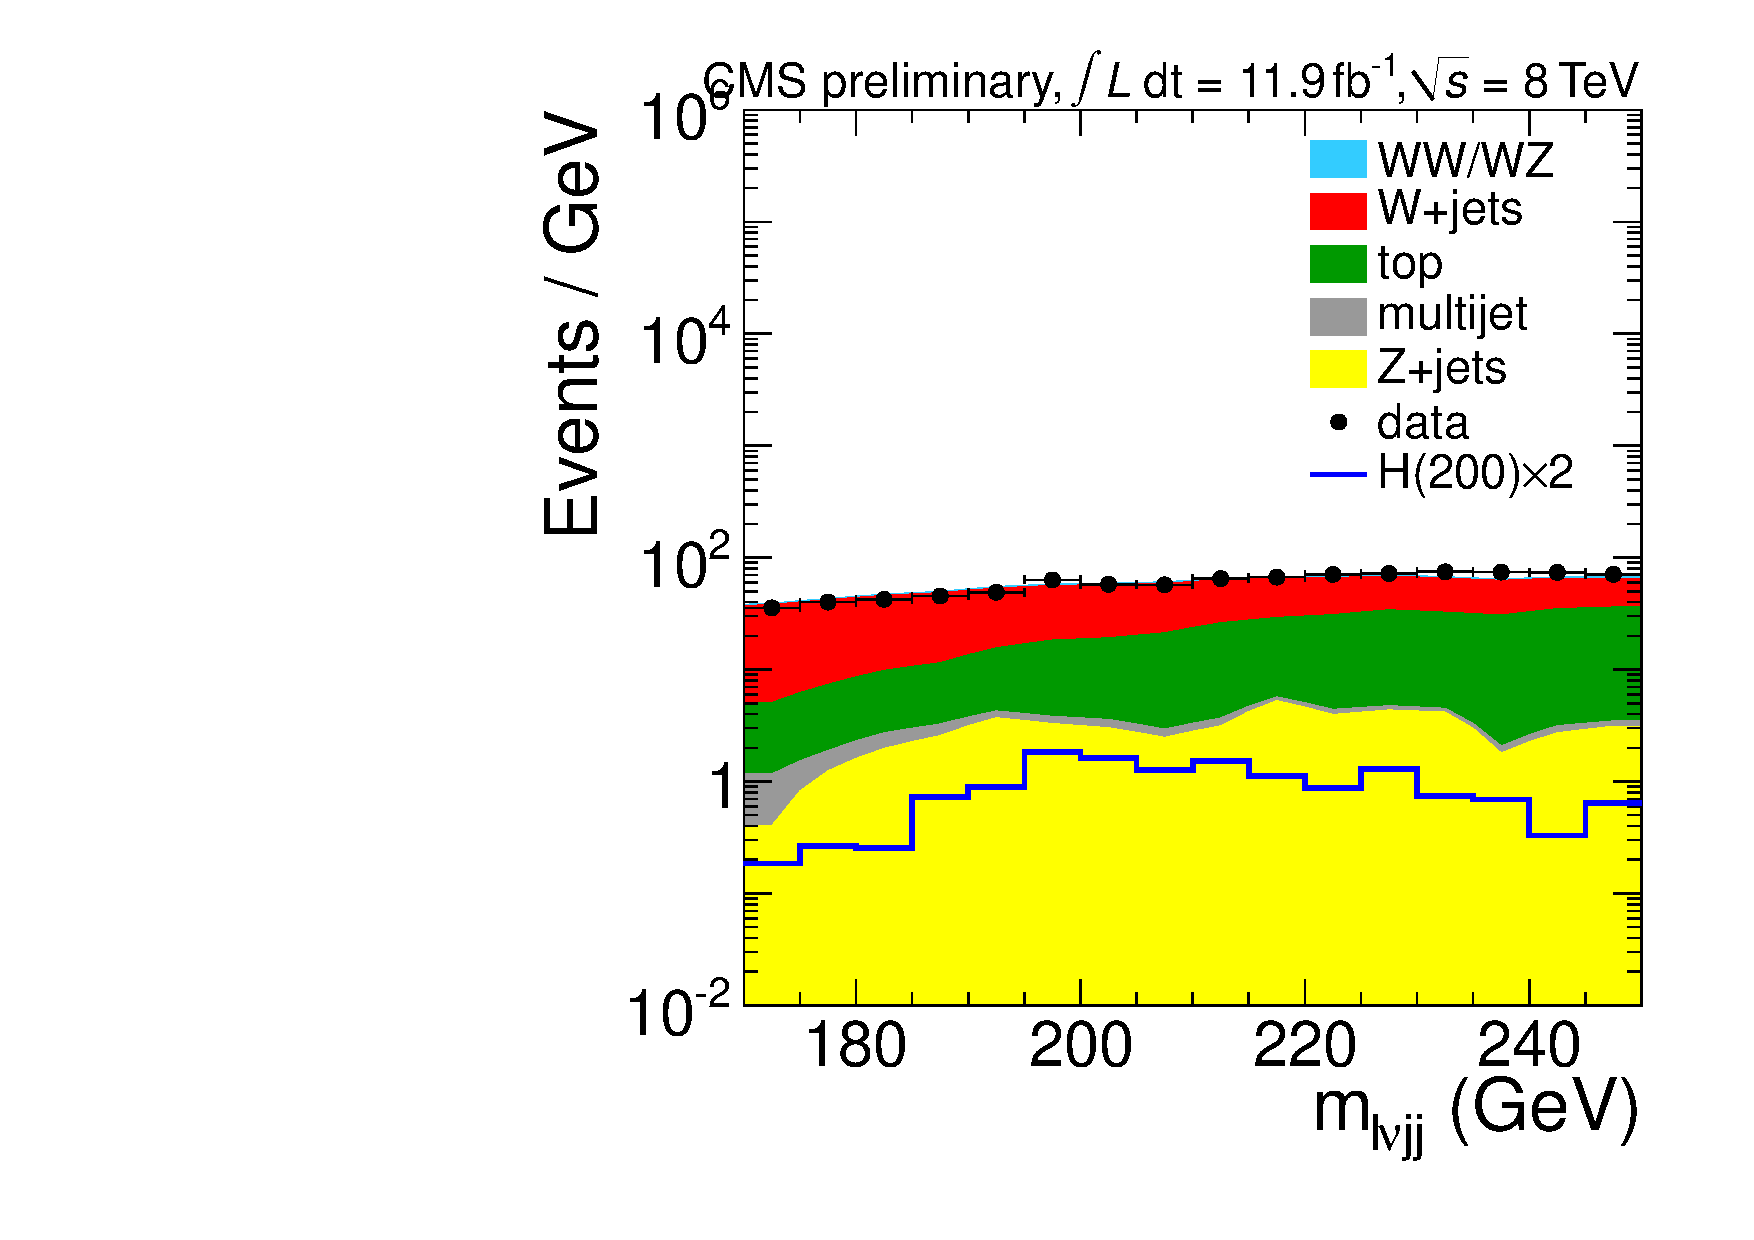
\includegraphics[width=0.45\textwidth]{plots/2012_FOURBSHAPES/H200_Mlvjj_Electron_3jets_Stacked_log}
%      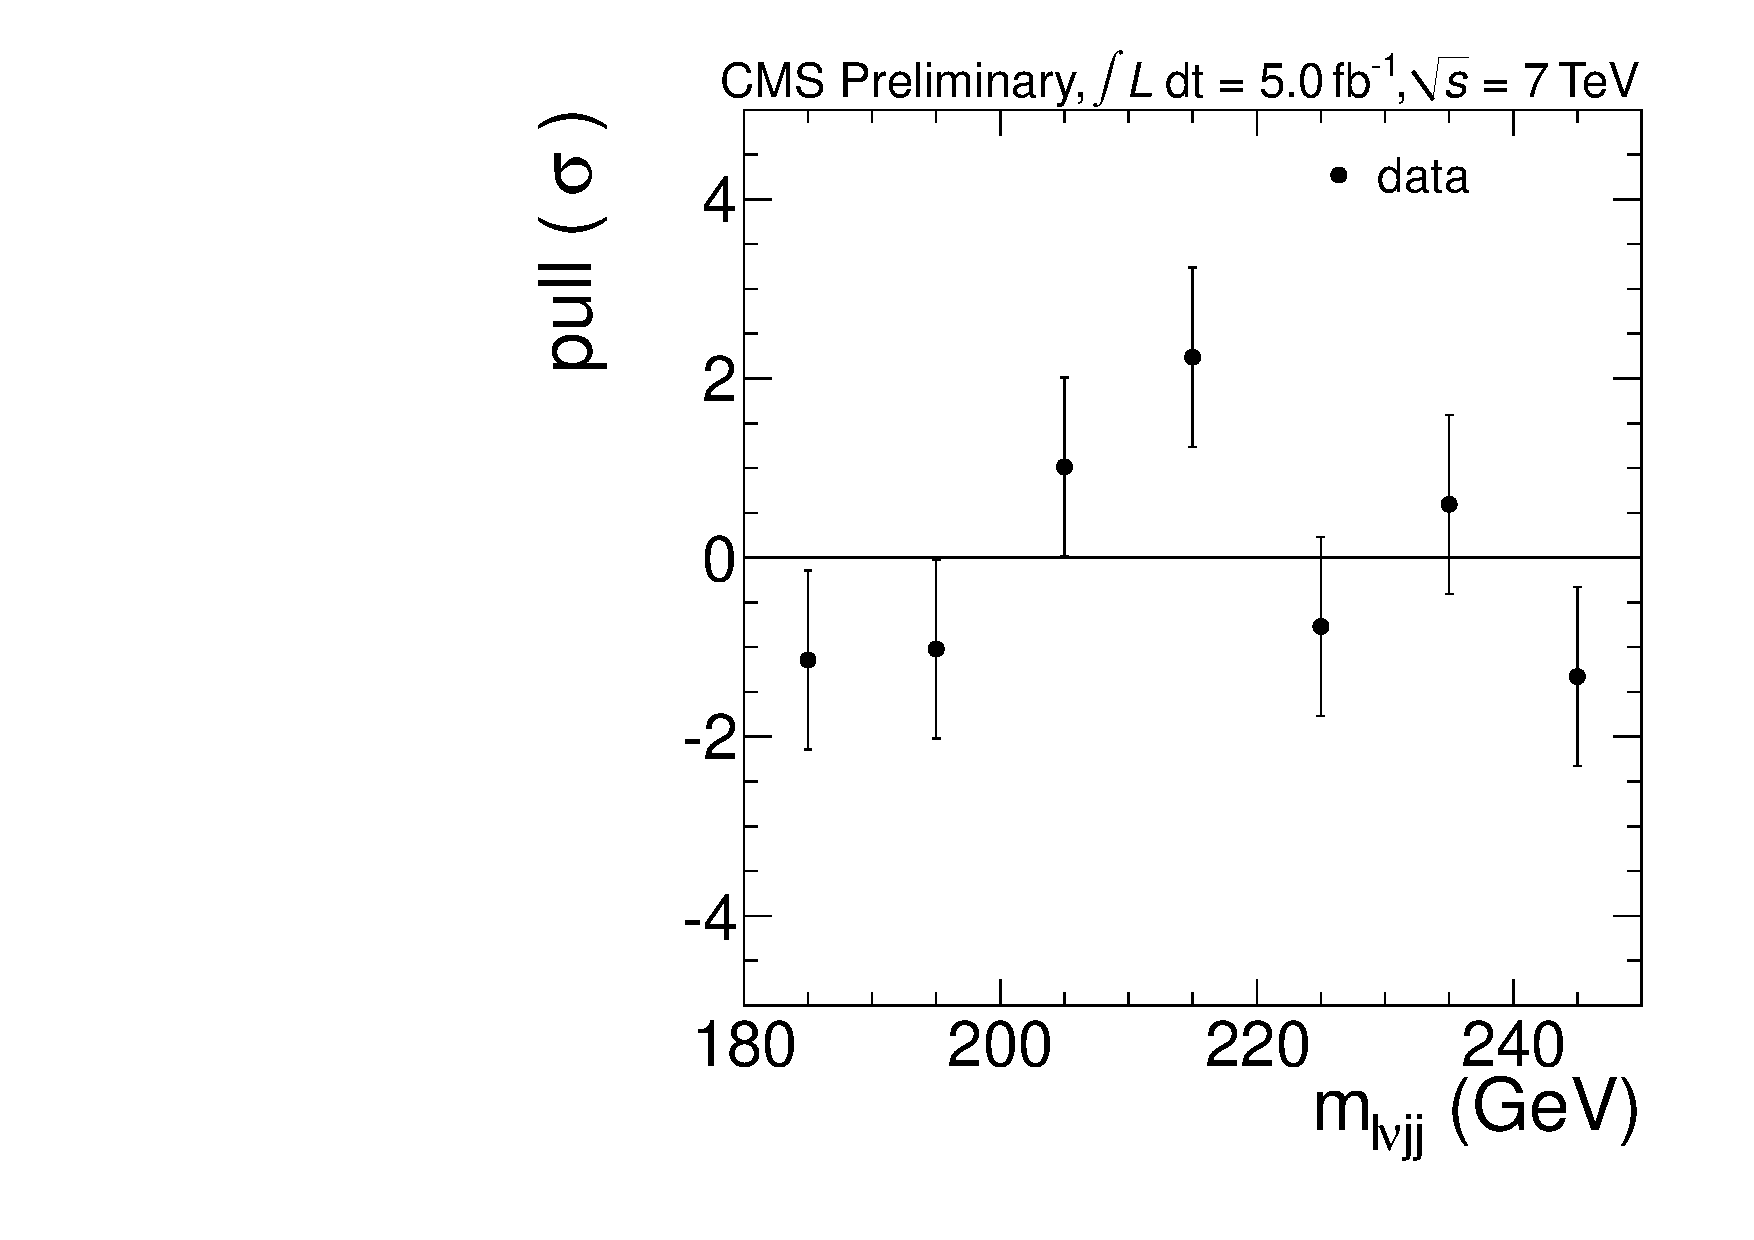
\includegraphics[width=0.3\textwidth]{plots/2012_FOURBSHAPES/H200_Mlvjj_Electron_3jets_Pull}
}
  \caption{The four-body mass distribution of data-driven background events in the signal regions for mass
  point M=200~GeV.}
  \label{fig:m4_dd_example200}
\end{figure}

\begin{figure}[!t]
  \centering
%% \subfigure[muon 2 jets, 350 GeV Higgs] {
%%      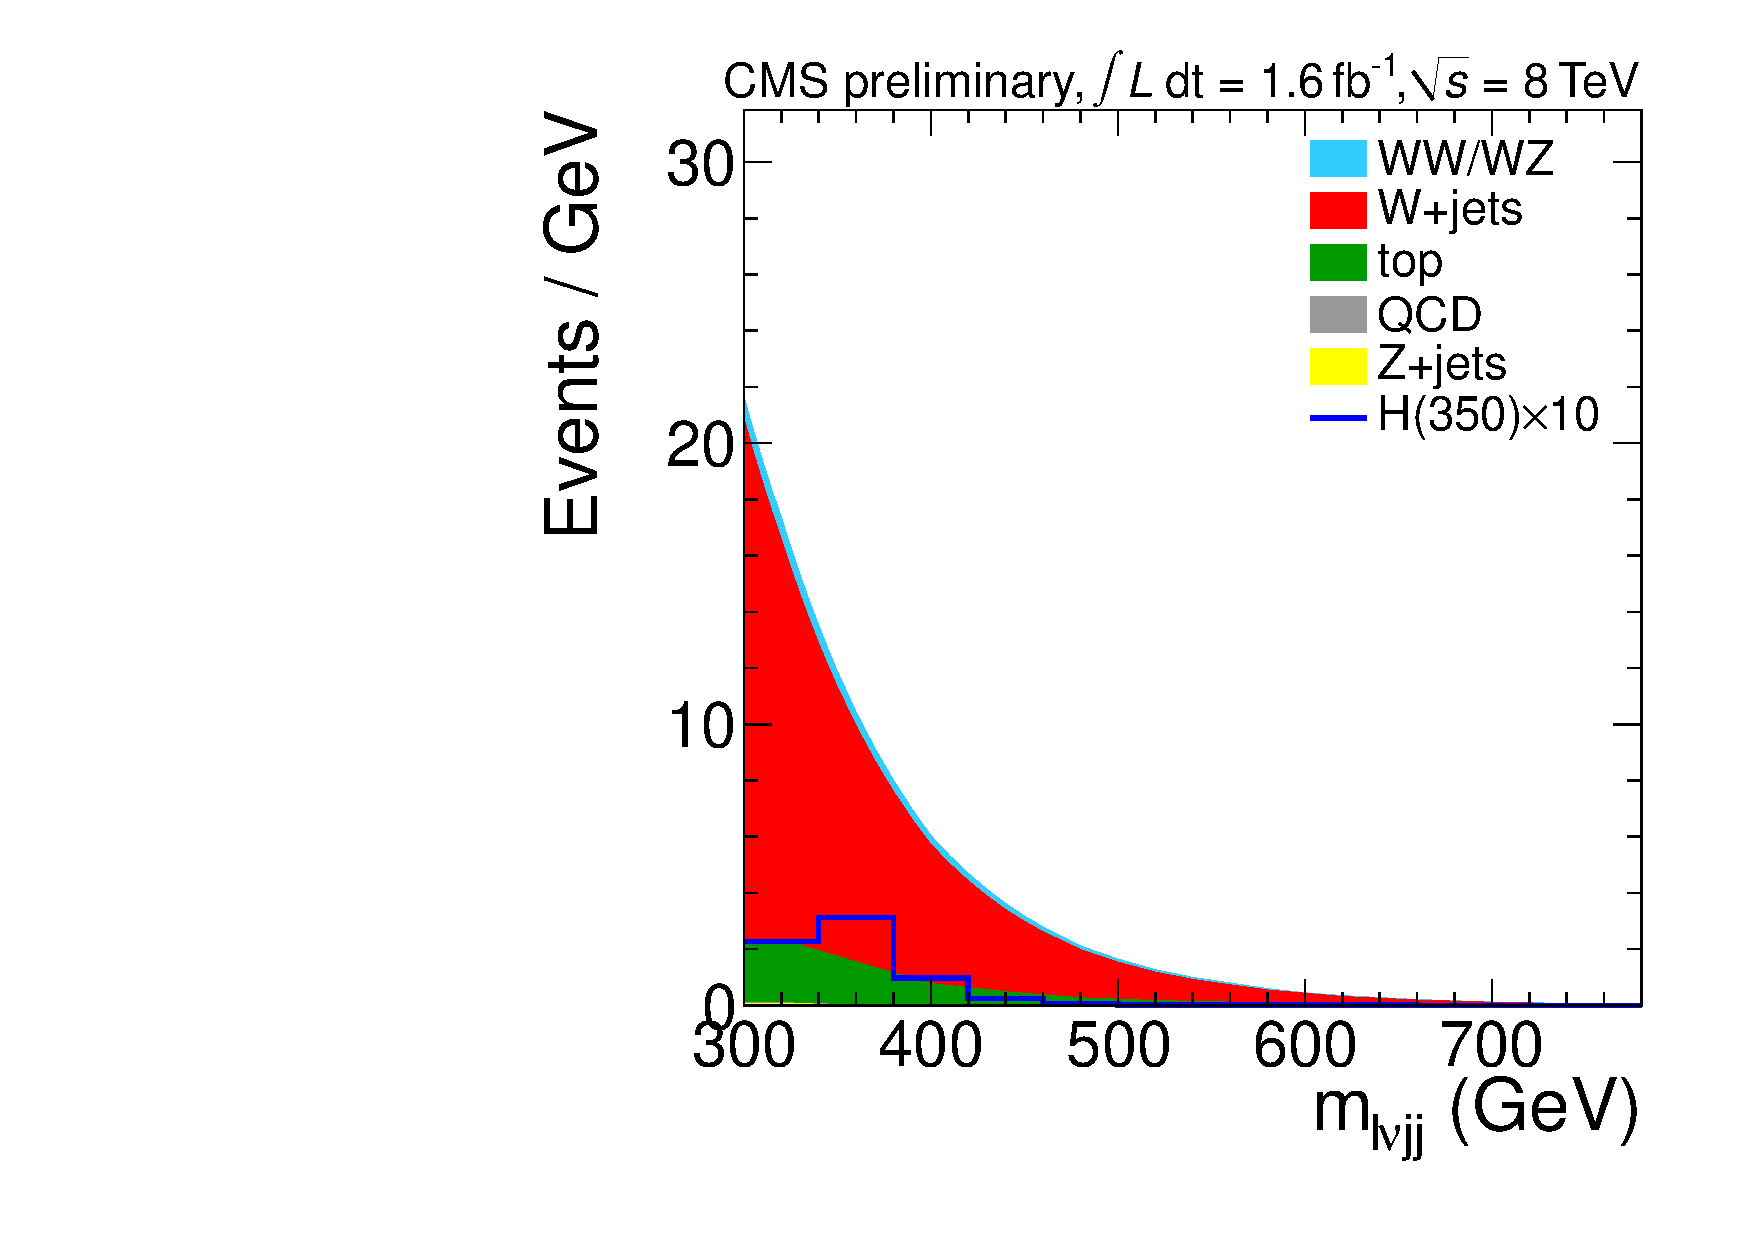
\includegraphics[width=0.3\textwidth]{plots/2012_FOURBSHAPES/H350_Mlvjj_Muon_2jets_Stacked}
%%      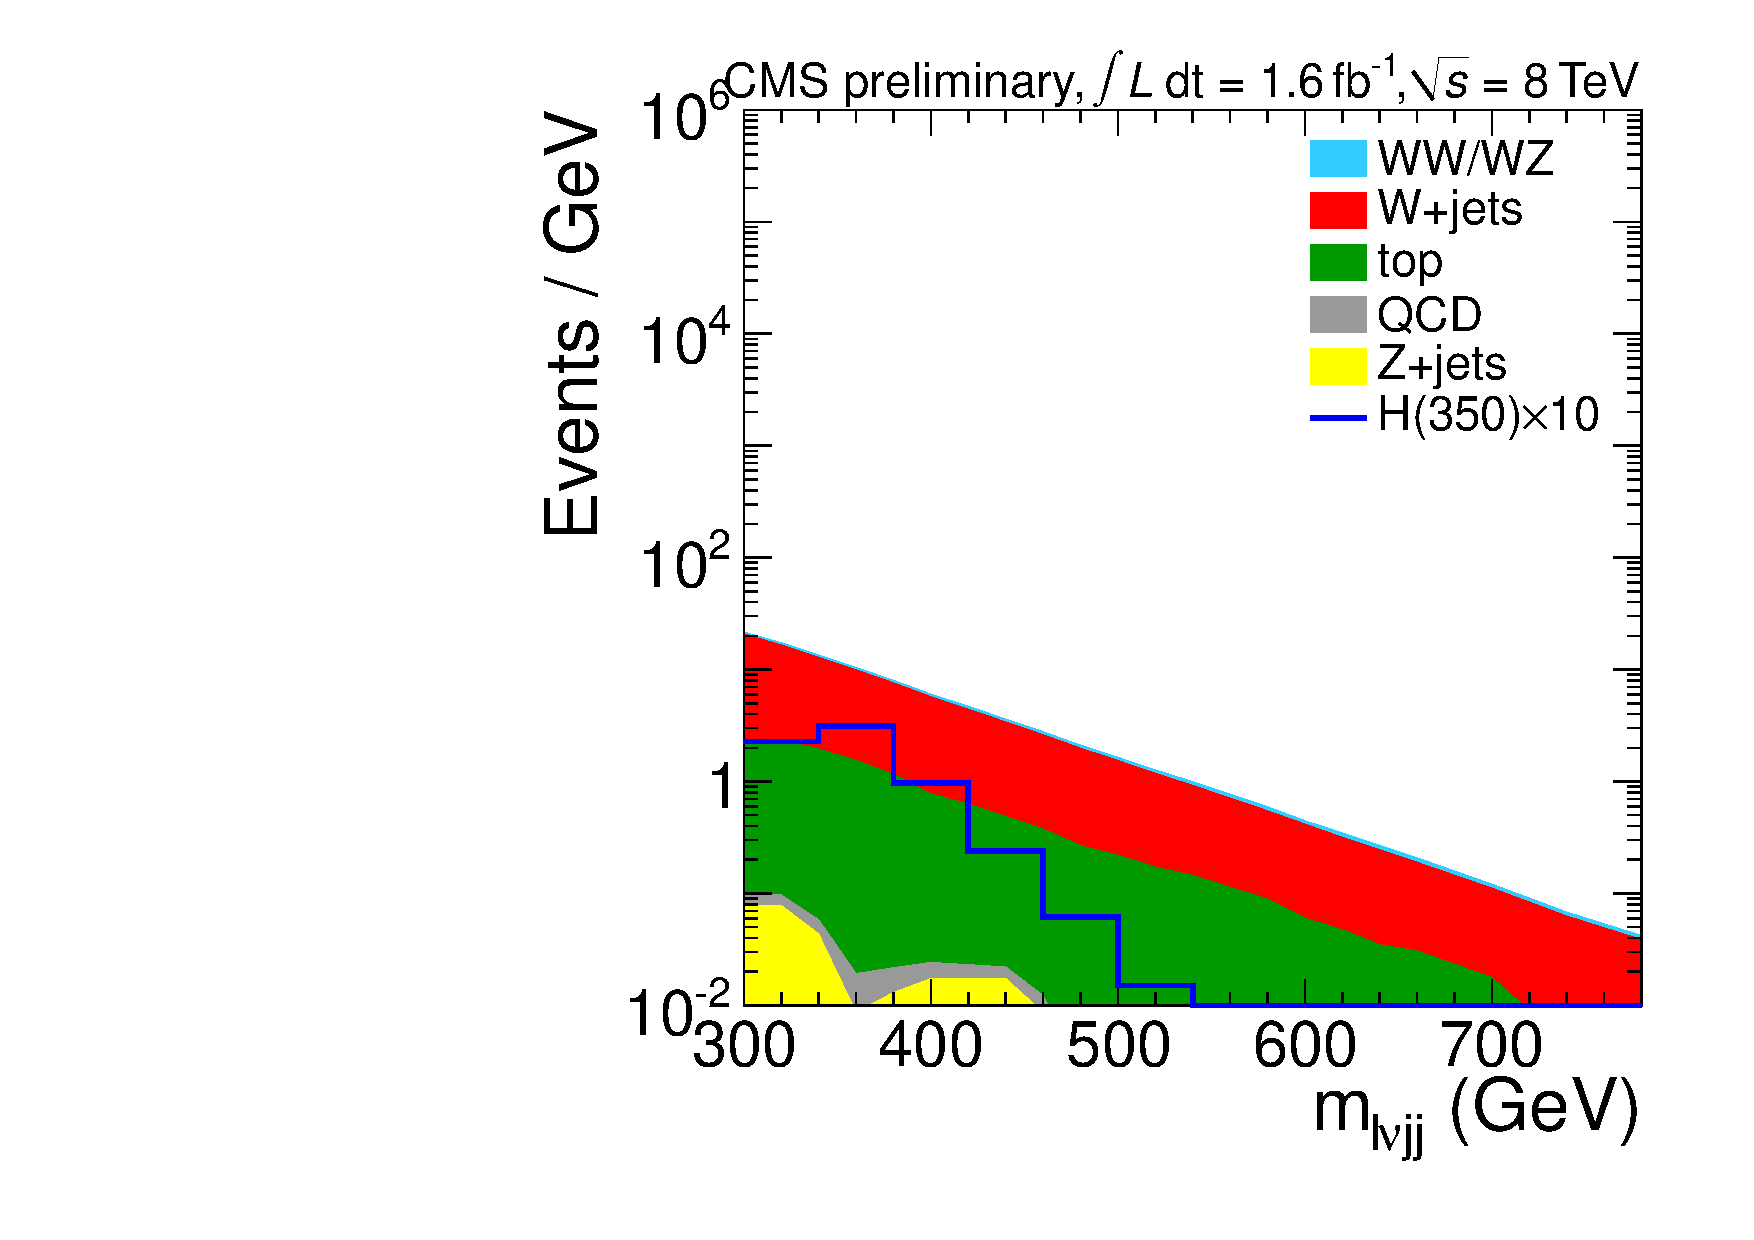
\includegraphics[width=0.3\textwidth]{plots/2012_FOURBSHAPES/H350_Mlvjj_Muon_2jets_Stacked_log}
\subfigure[muon 2 jets, 300 GeV Higgs] {
     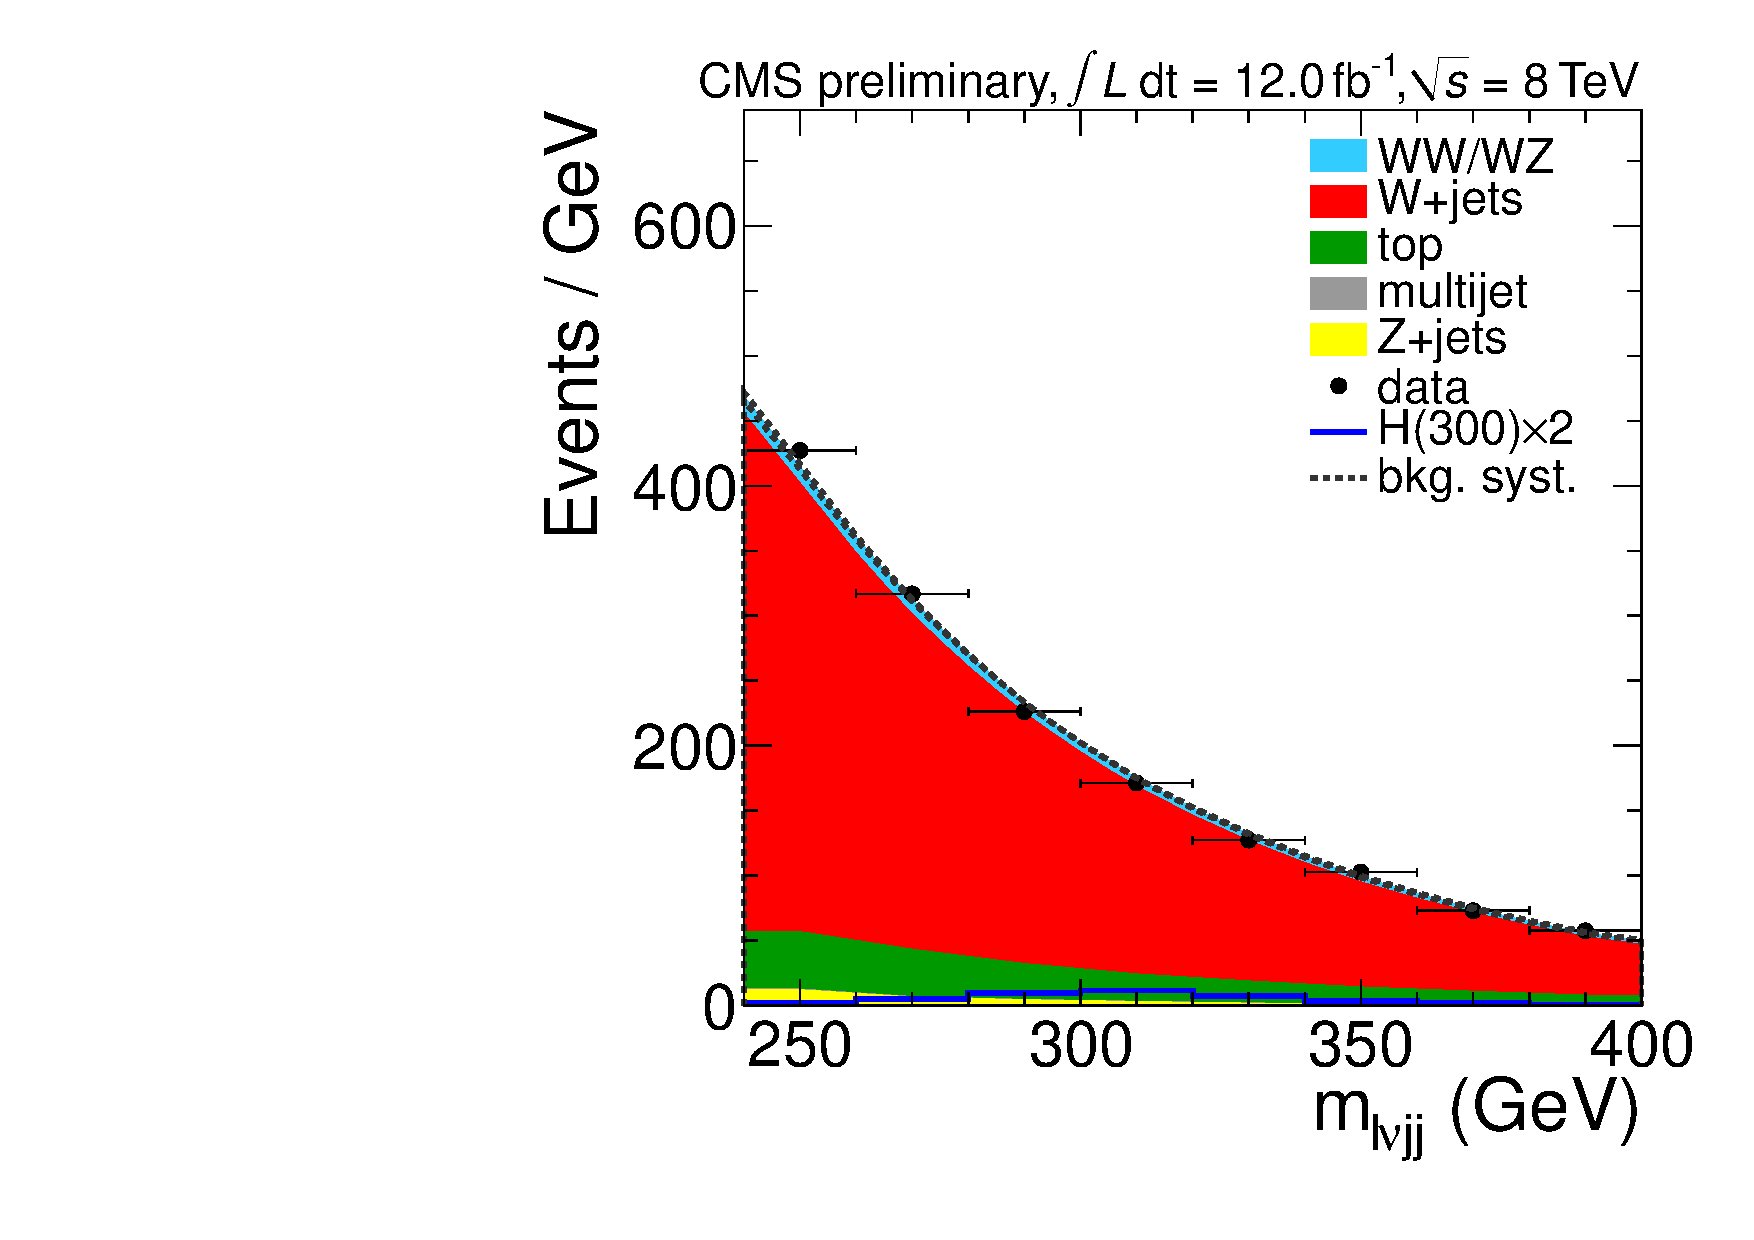
\includegraphics[width=0.45\textwidth]{plots/2012_FOURBSHAPES/H300_Mlvjj_Muon_2jets_Stacked}
     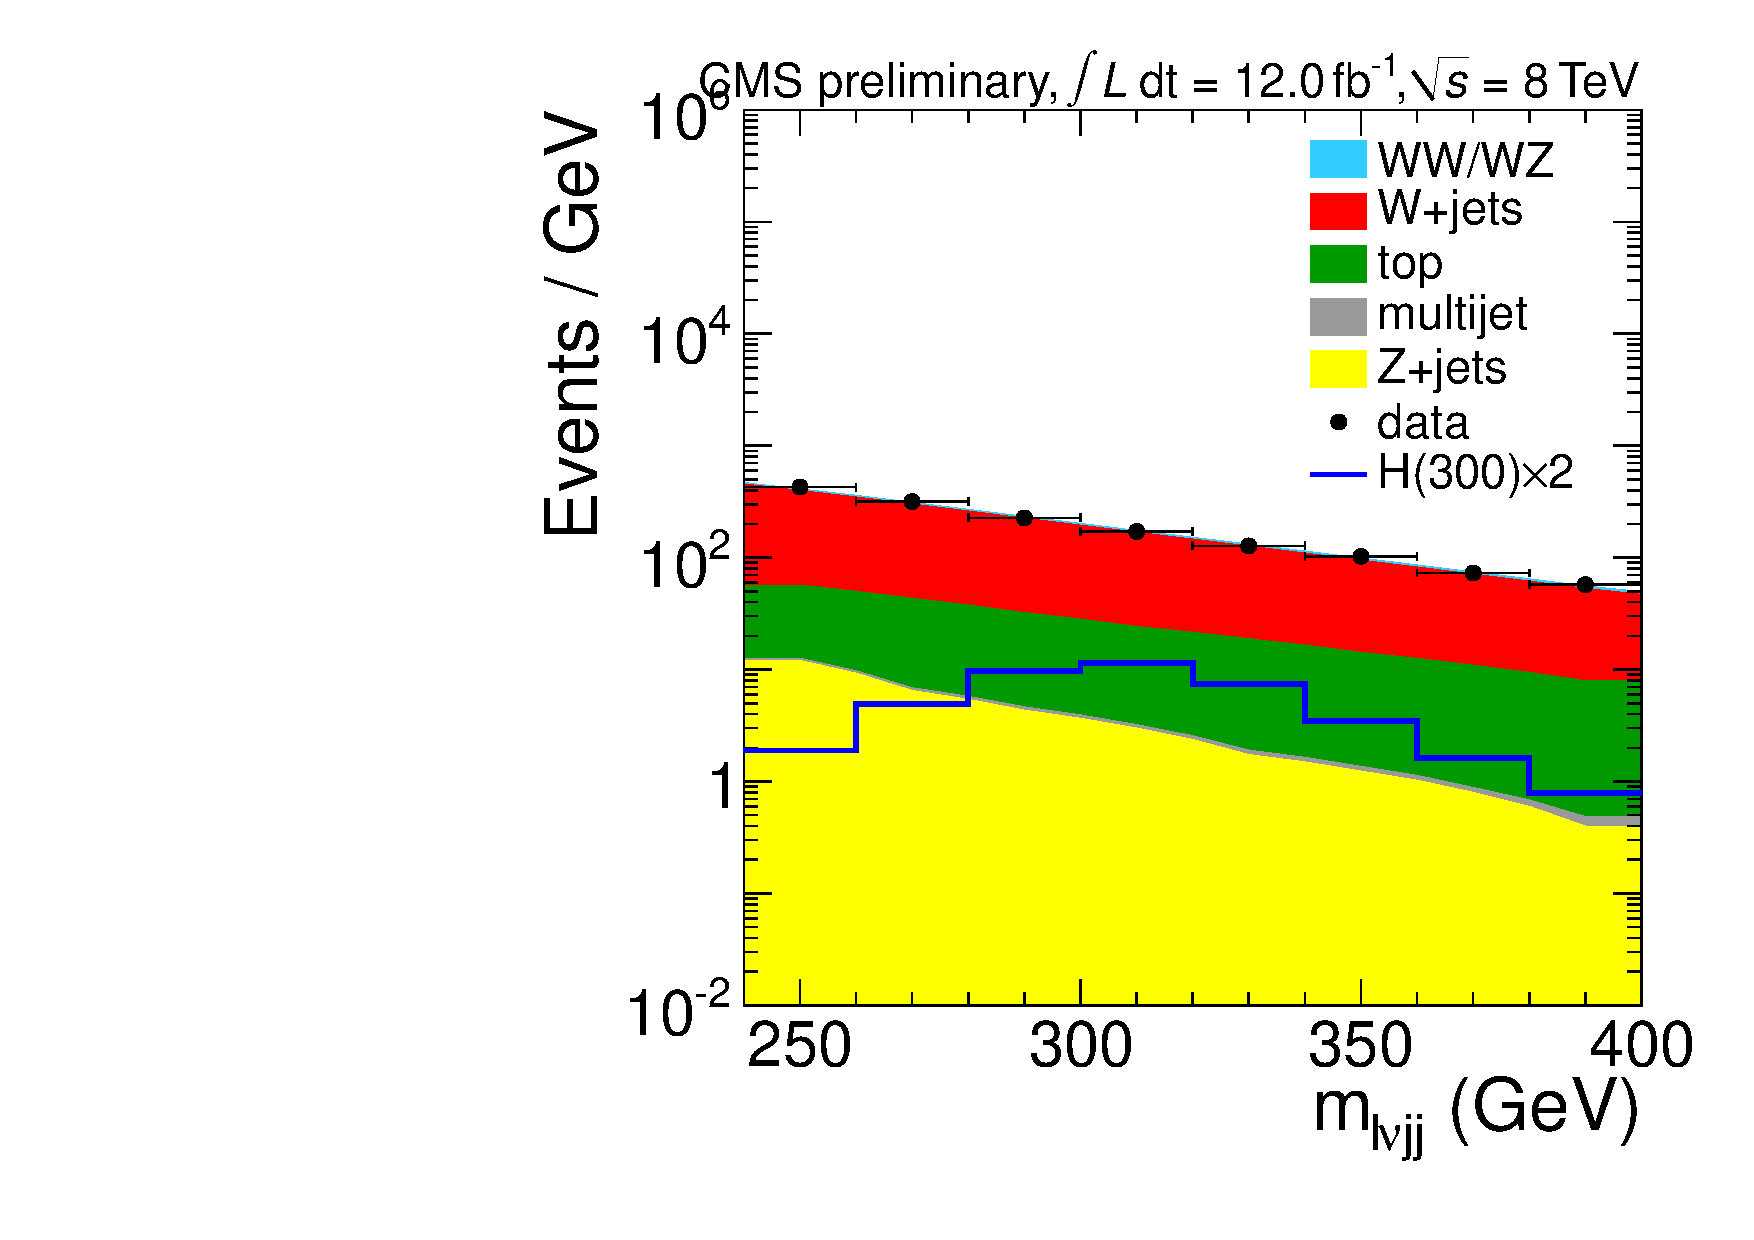
\includegraphics[width=0.45\textwidth]{plots/2012_FOURBSHAPES/H300_Mlvjj_Muon_2jets_Stacked_log}
%%     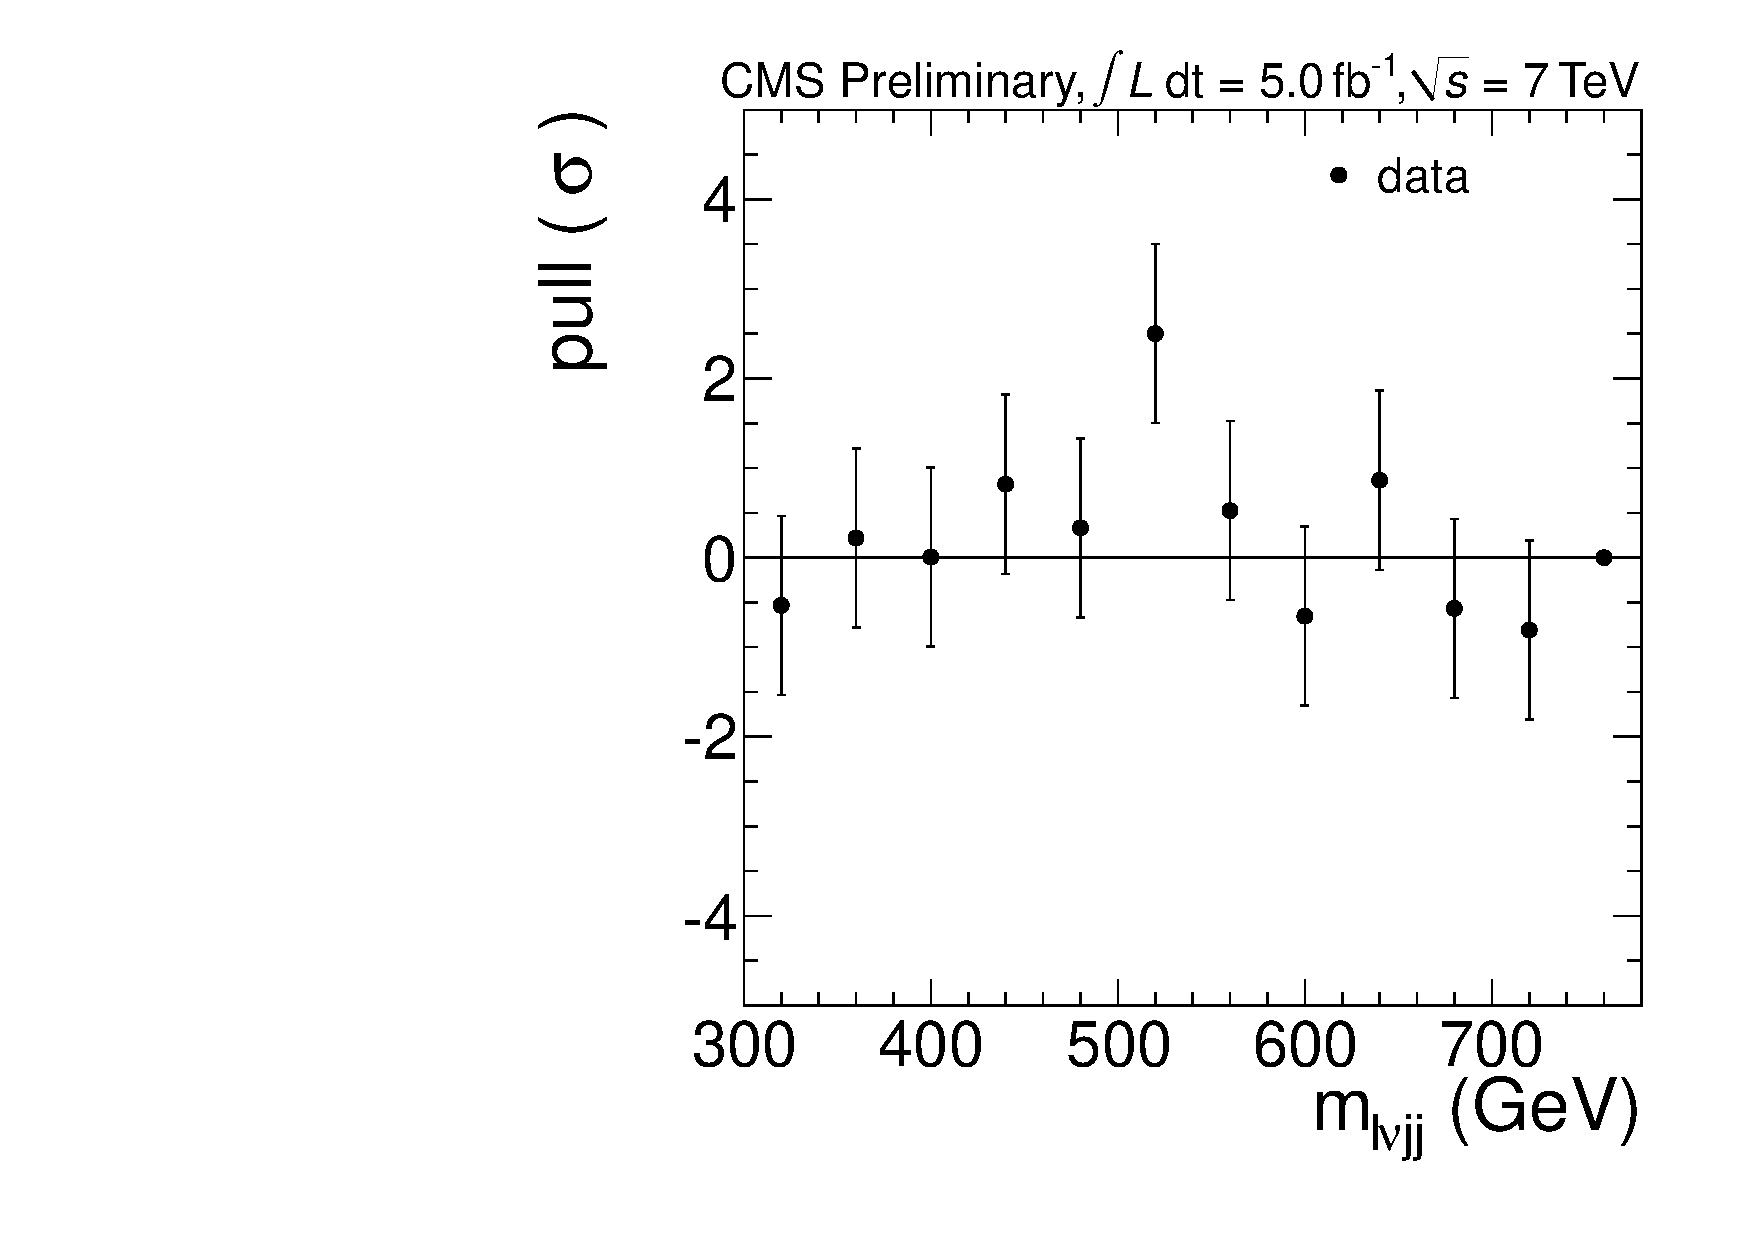
\includegraphics[width=0.3\textwidth]{plots/2012_FOURBSHAPES/H350_Mlvjj_Muon_2jets_Pull}
}

%% \subfigure[muon 3 jets, 350 GeV Higgs] {
%%      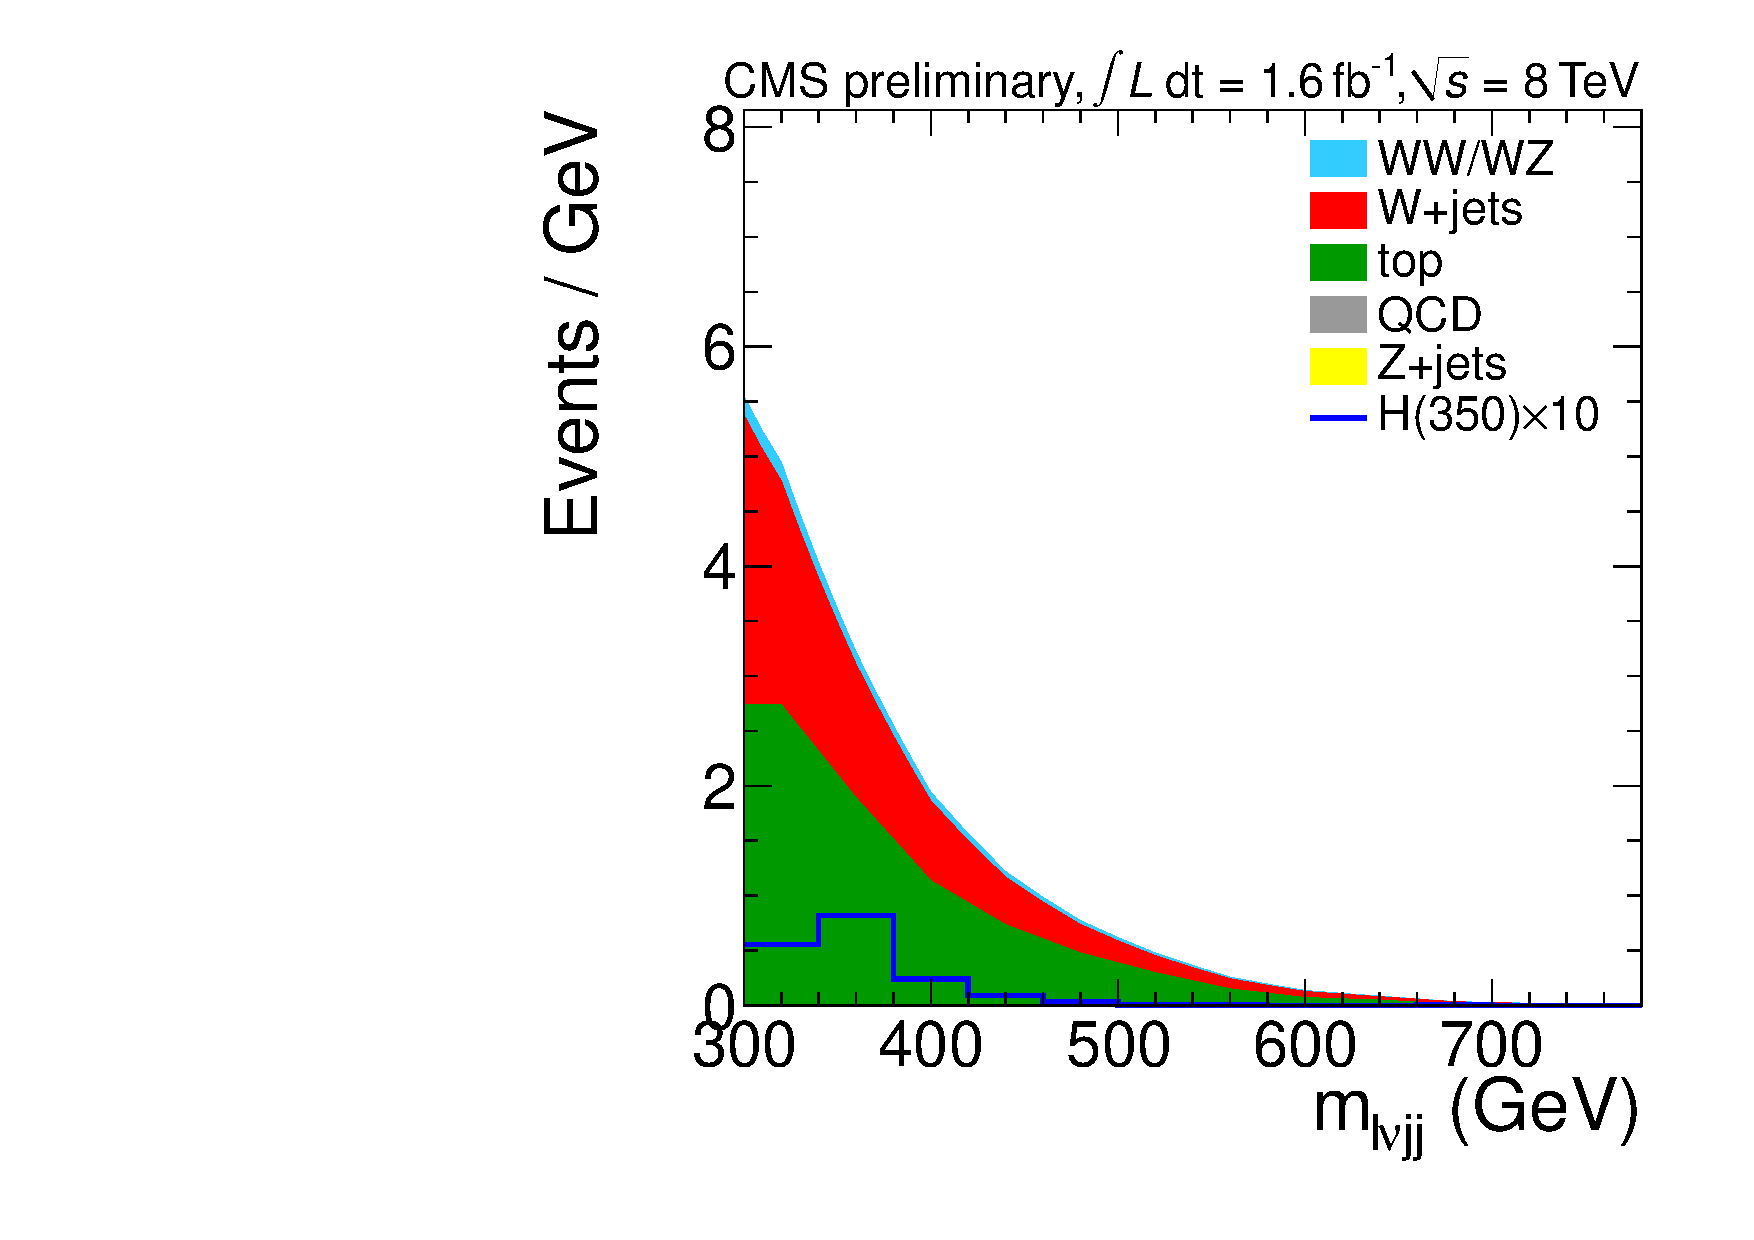
\includegraphics[width=0.3\textwidth]{plots/2012_FOURBSHAPES/H350_Mlvjj_Muon_3jets_Stacked}
%%      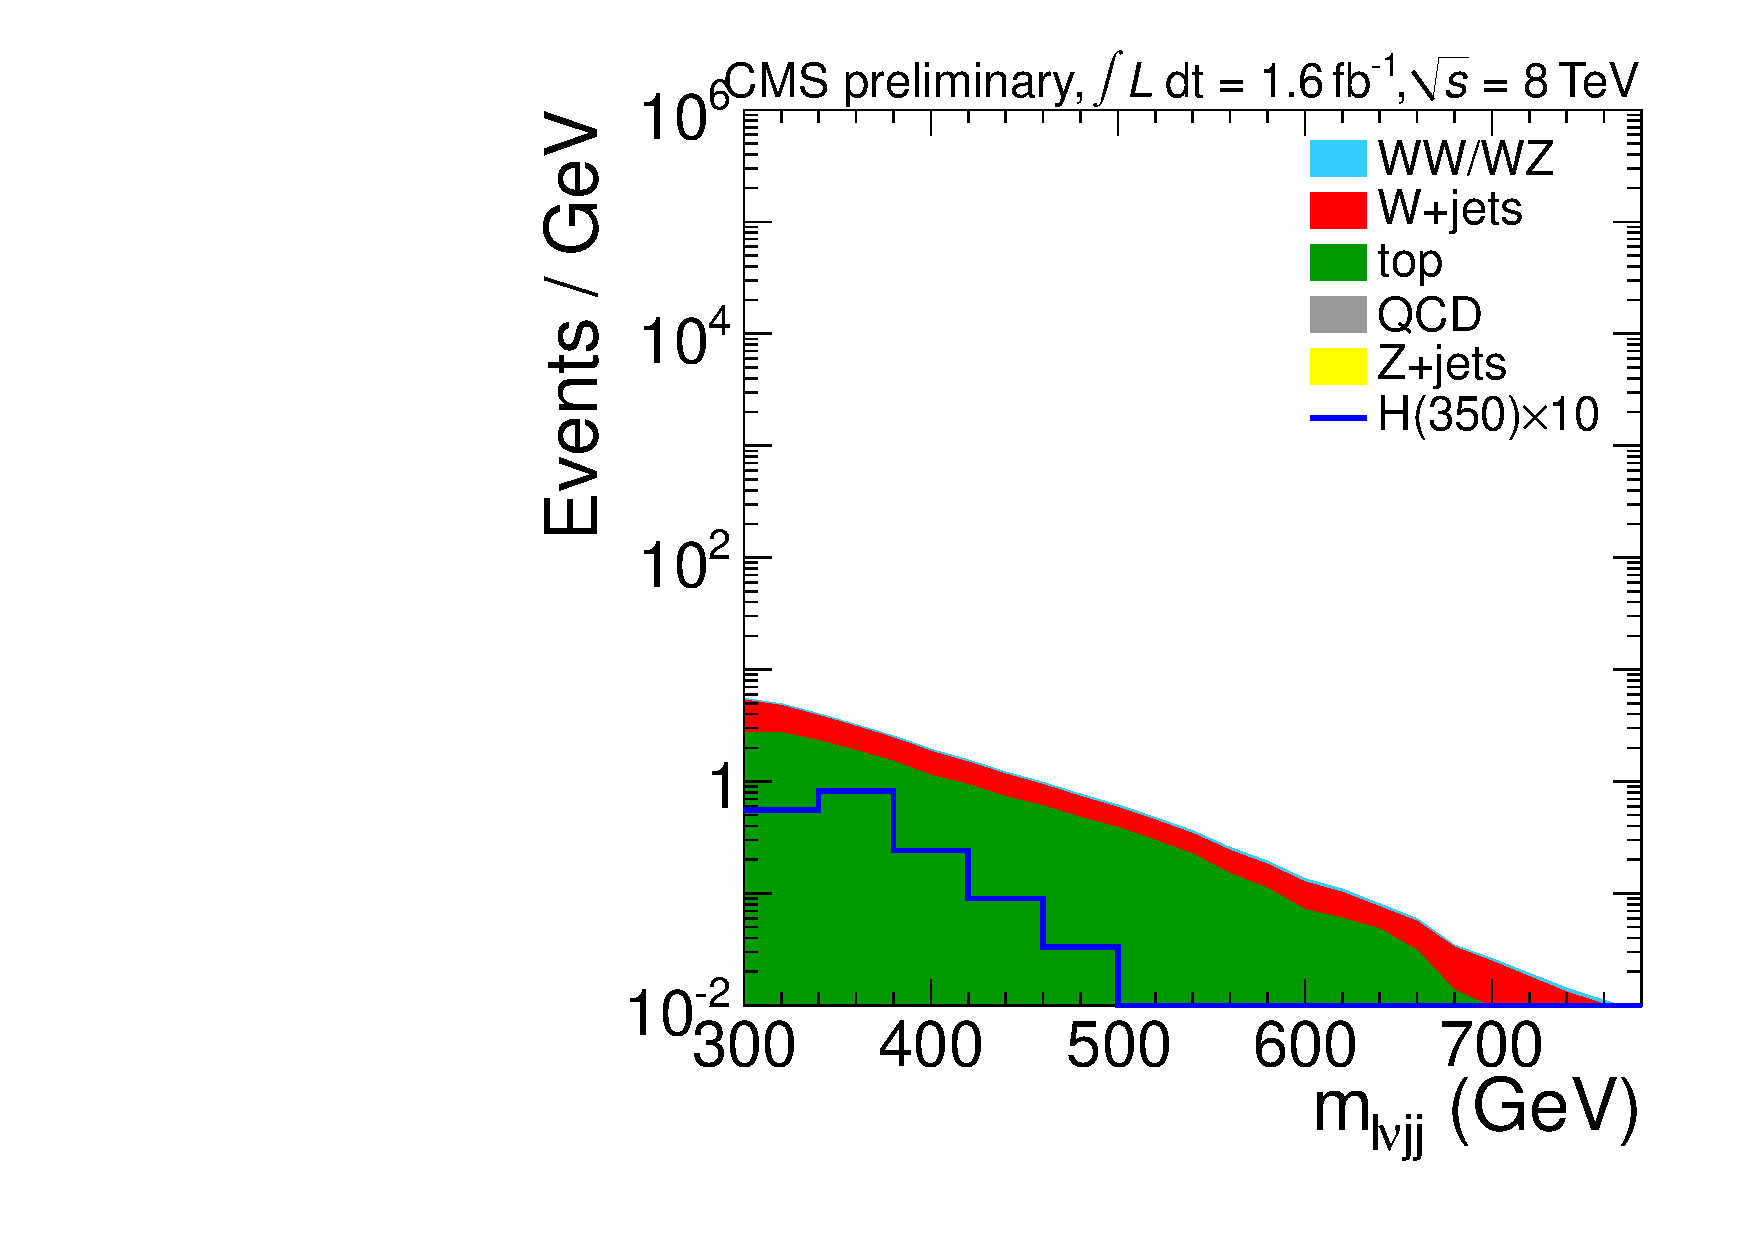
\includegraphics[width=0.3\textwidth]{plots/2012_FOURBSHAPES/H350_Mlvjj_Muon_3jets_Stacked_log}
\subfigure[muon 3 jets, 300 GeV Higgs] {
     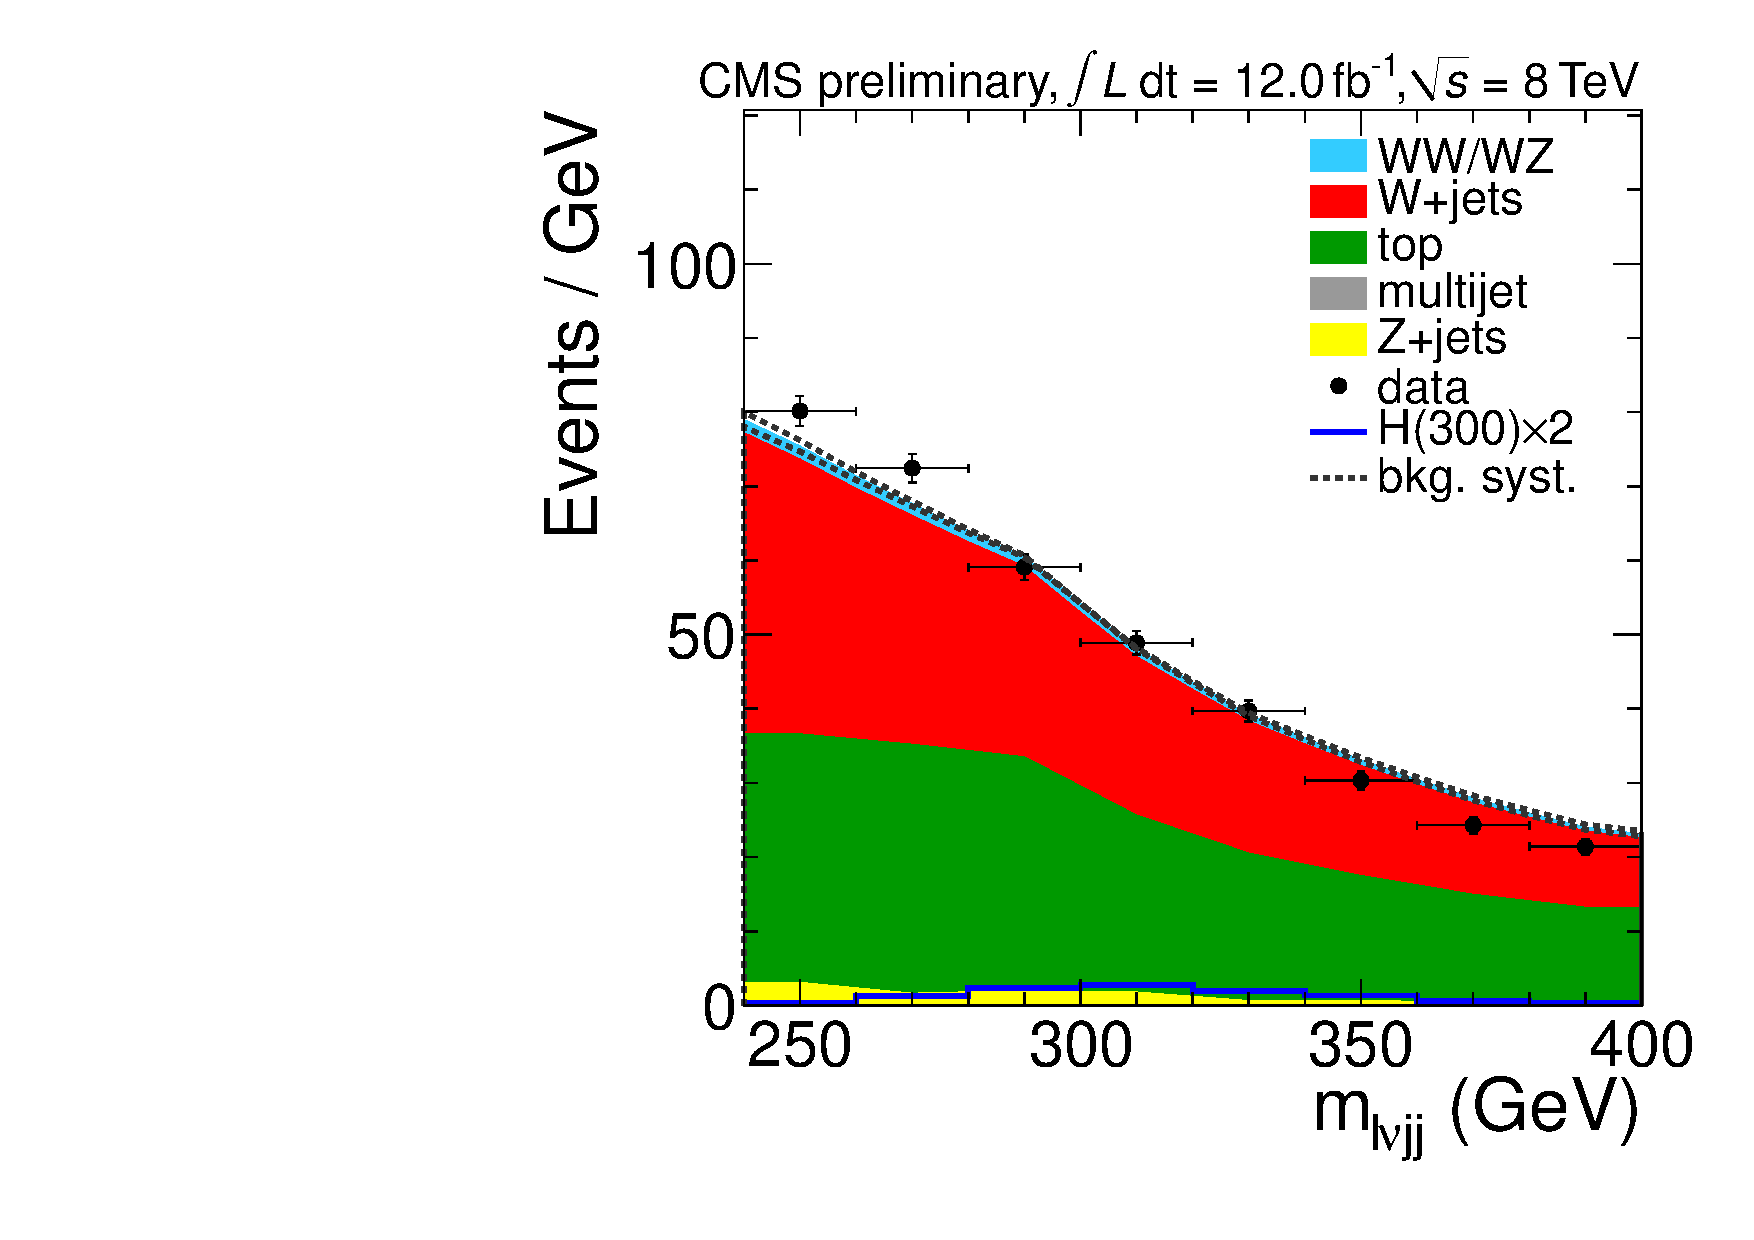
\includegraphics[width=0.45\textwidth]{plots/2012_FOURBSHAPES/H300_Mlvjj_Muon_3jets_Stacked}
     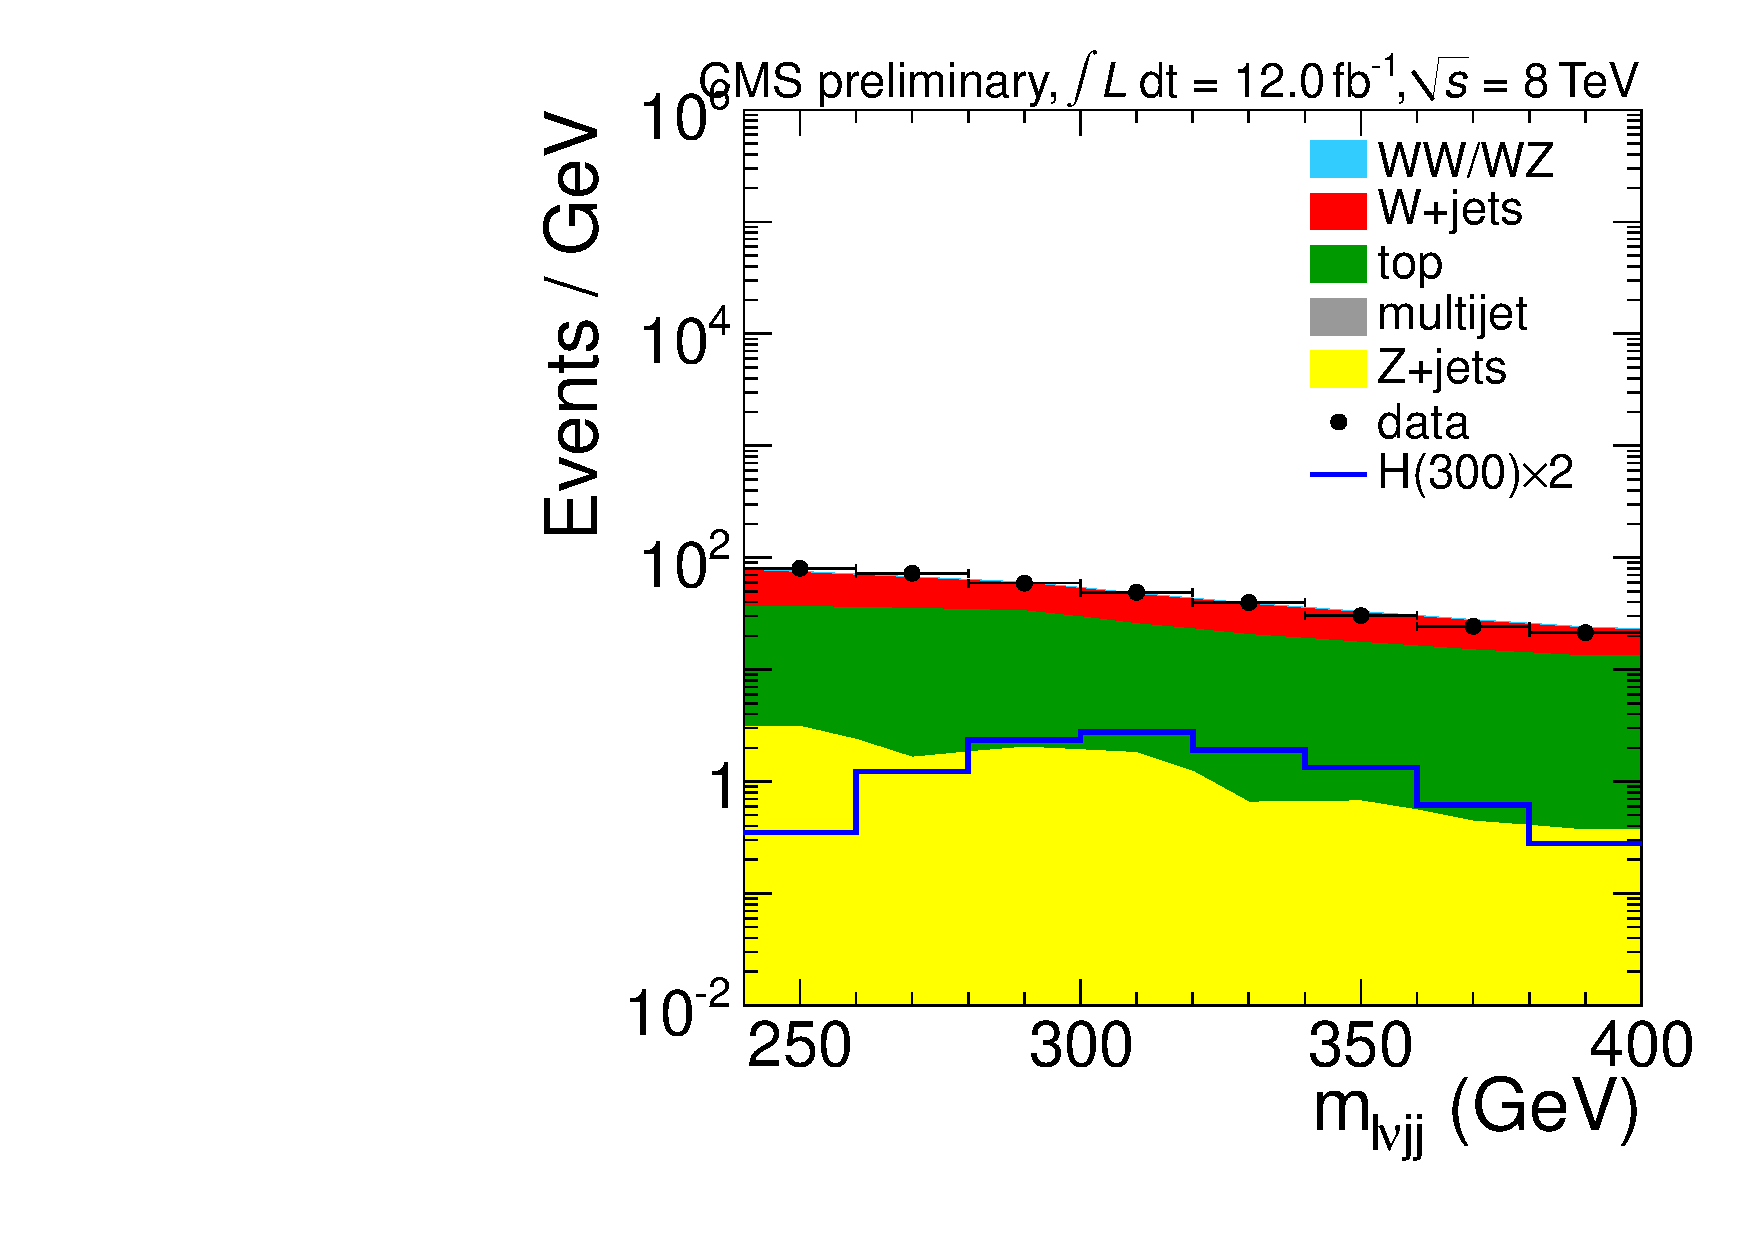
\includegraphics[width=0.45\textwidth]{plots/2012_FOURBSHAPES/H300_Mlvjj_Muon_3jets_Stacked_log}
%%     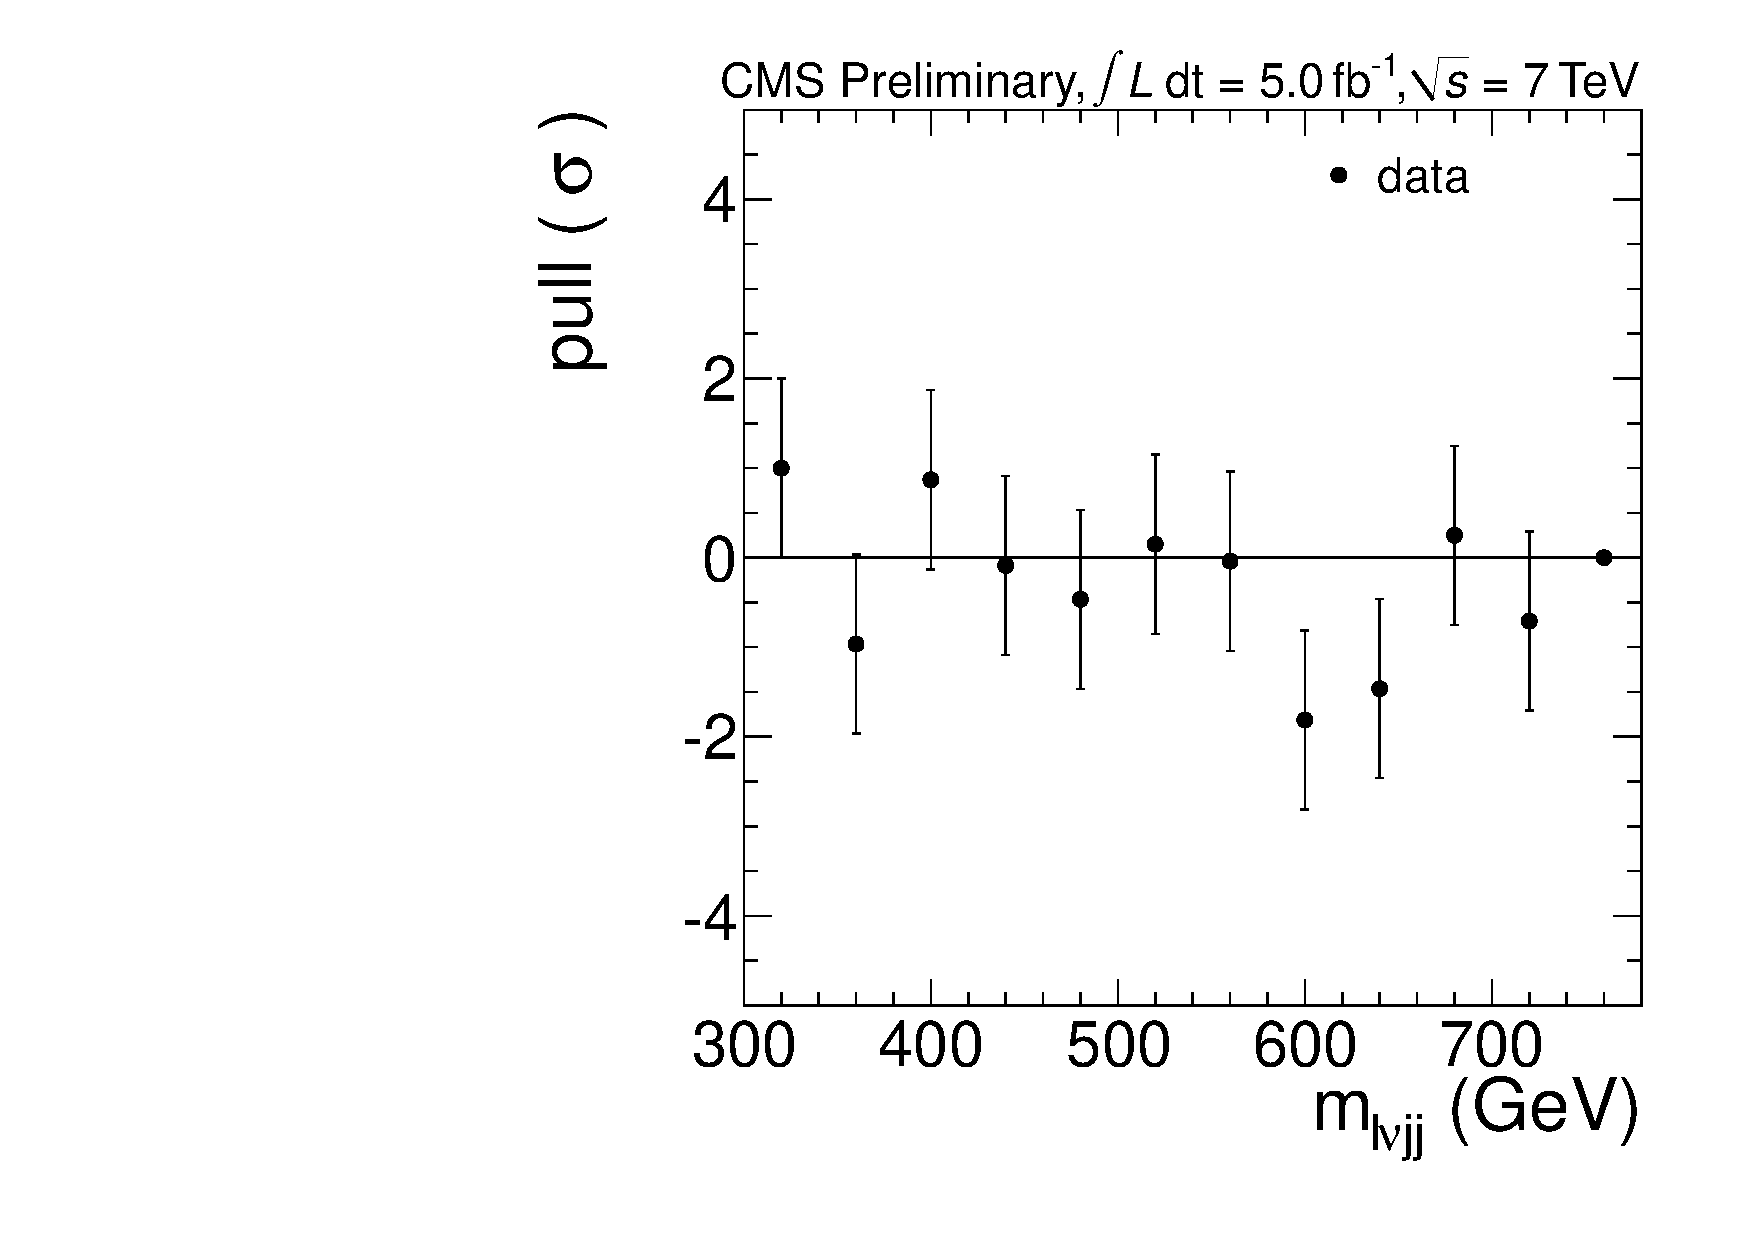
\includegraphics[width=0.3\textwidth]{plots/2012_FOURBSHAPES/H350_Mlvjj_Muon_3jets_Pull}
}
  \caption{The four-body mass distribution of data-driven background events in the signal regions for mass
  point M=300~GeV.}
  \label{fig:m4_dd_example300}
\end{figure}

\begin{figure}[!t]
  \centering
\subfigure[muon 2 jets, 500 GeV Higgs] {
     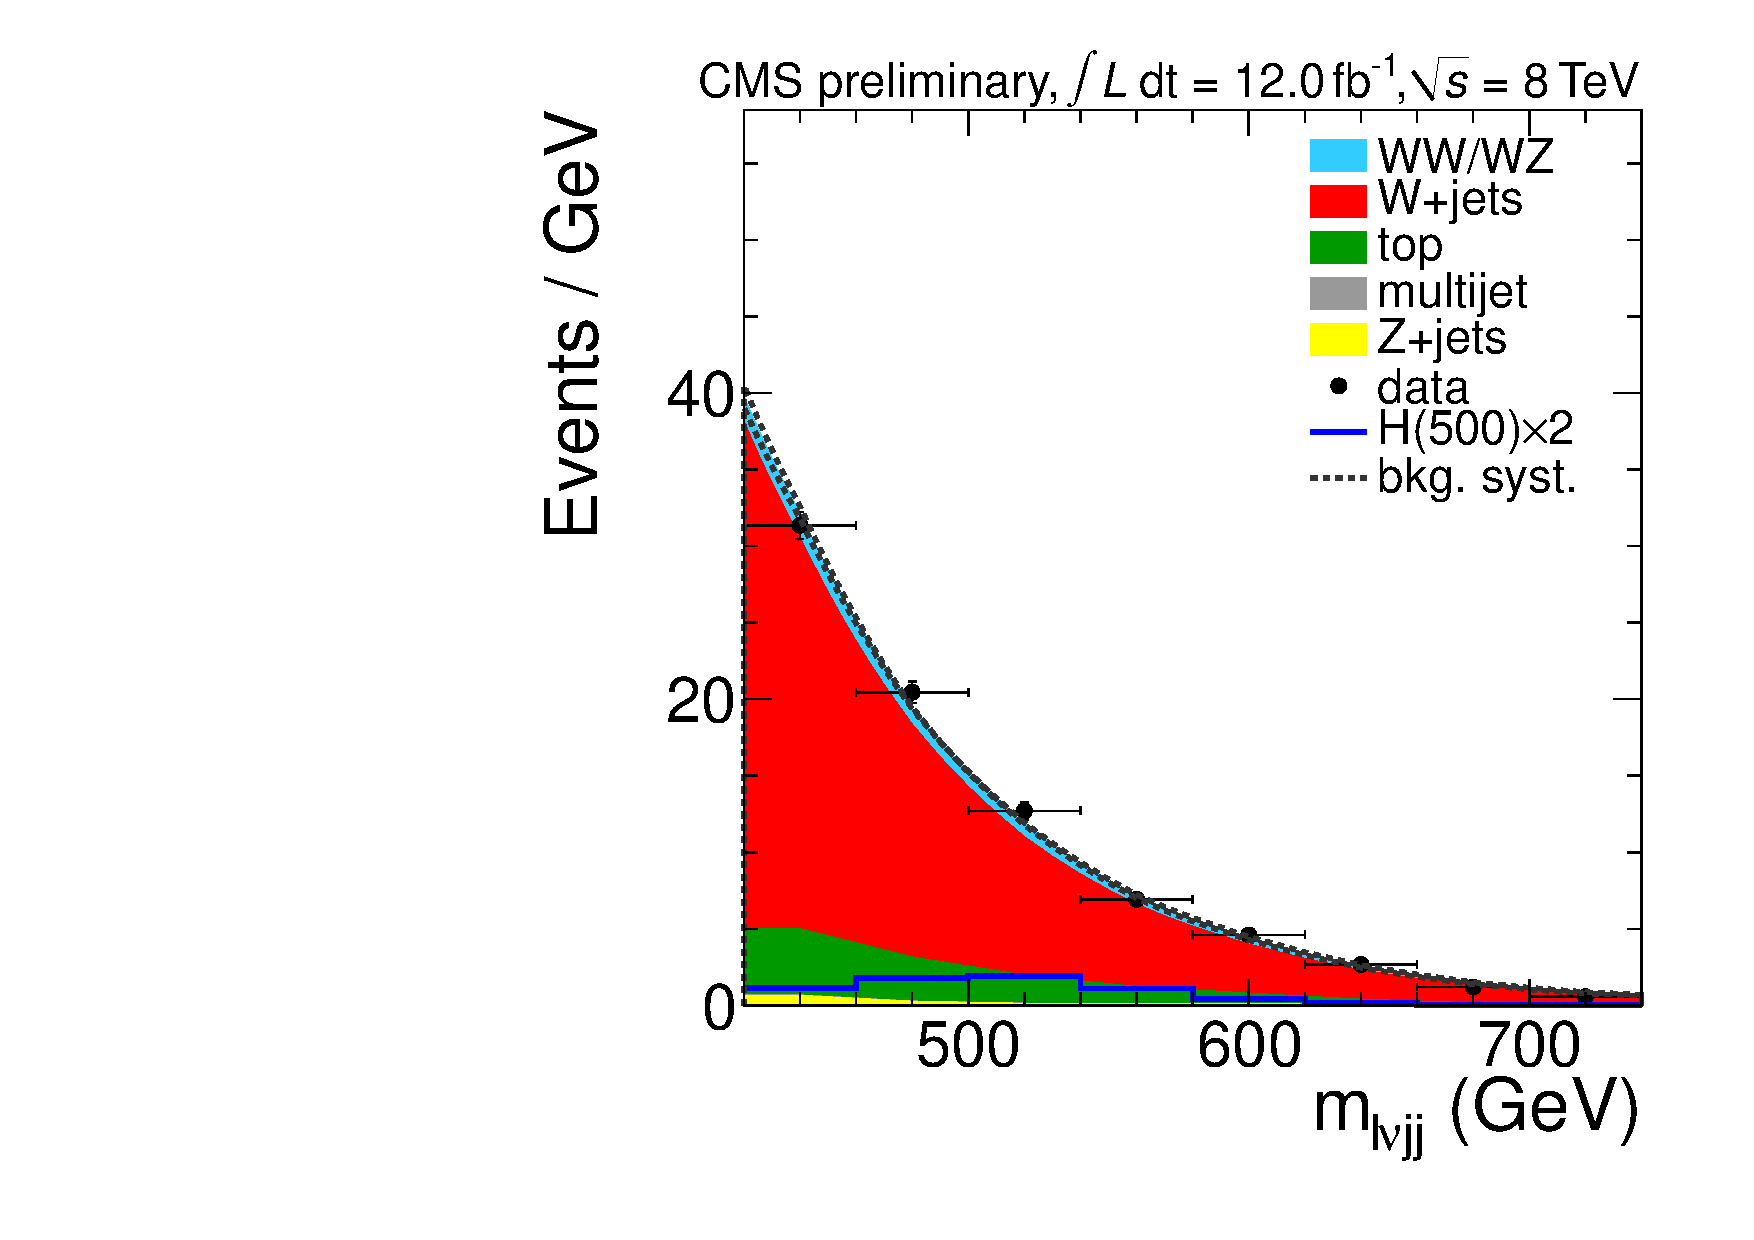
\includegraphics[width=0.45\textwidth]{plots/2012_FOURBSHAPES/H500_Mlvjj_Muon_2jets_Stacked}
     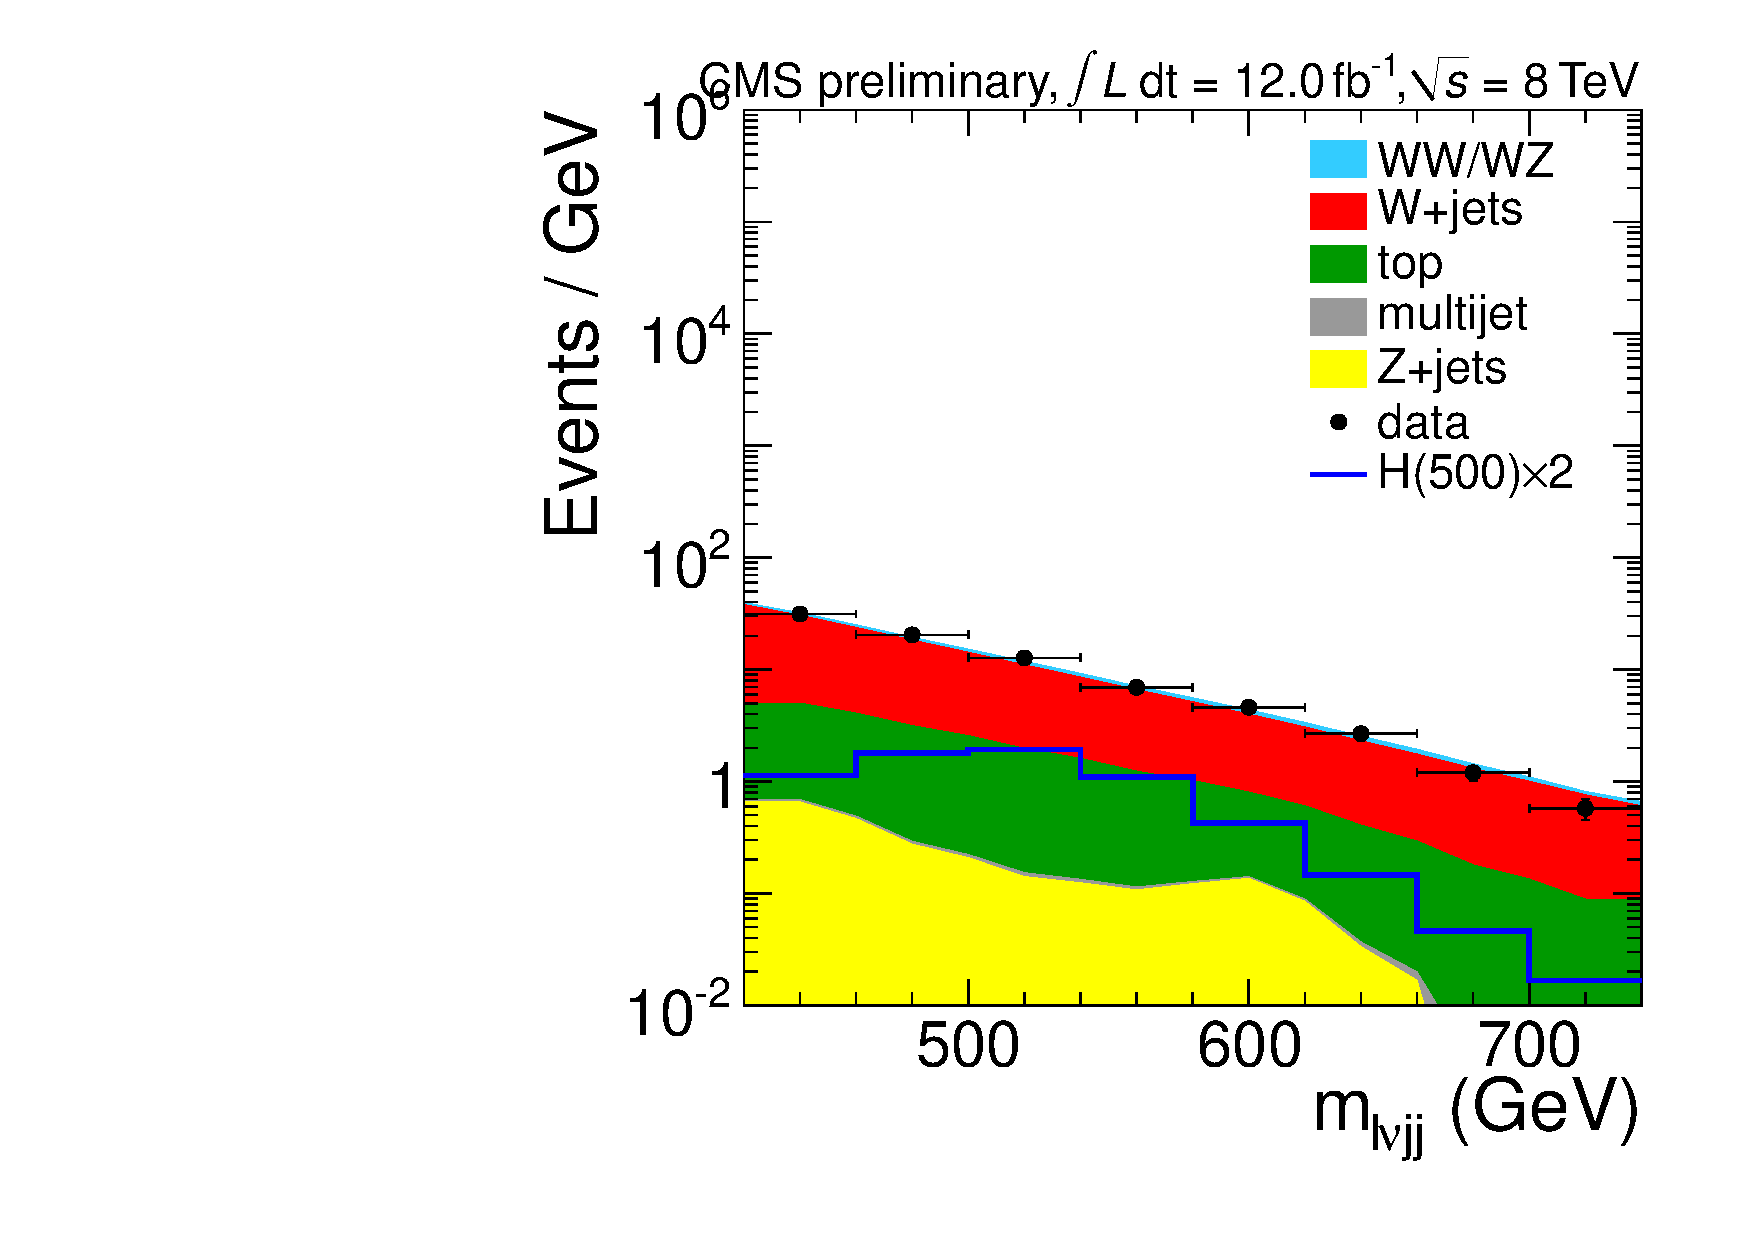
\includegraphics[width=0.45\textwidth]{plots/2012_FOURBSHAPES/H500_Mlvjj_Muon_2jets_Stacked_log}
}

\subfigure[muon 3 jets, 500 GeV Higgs] {
     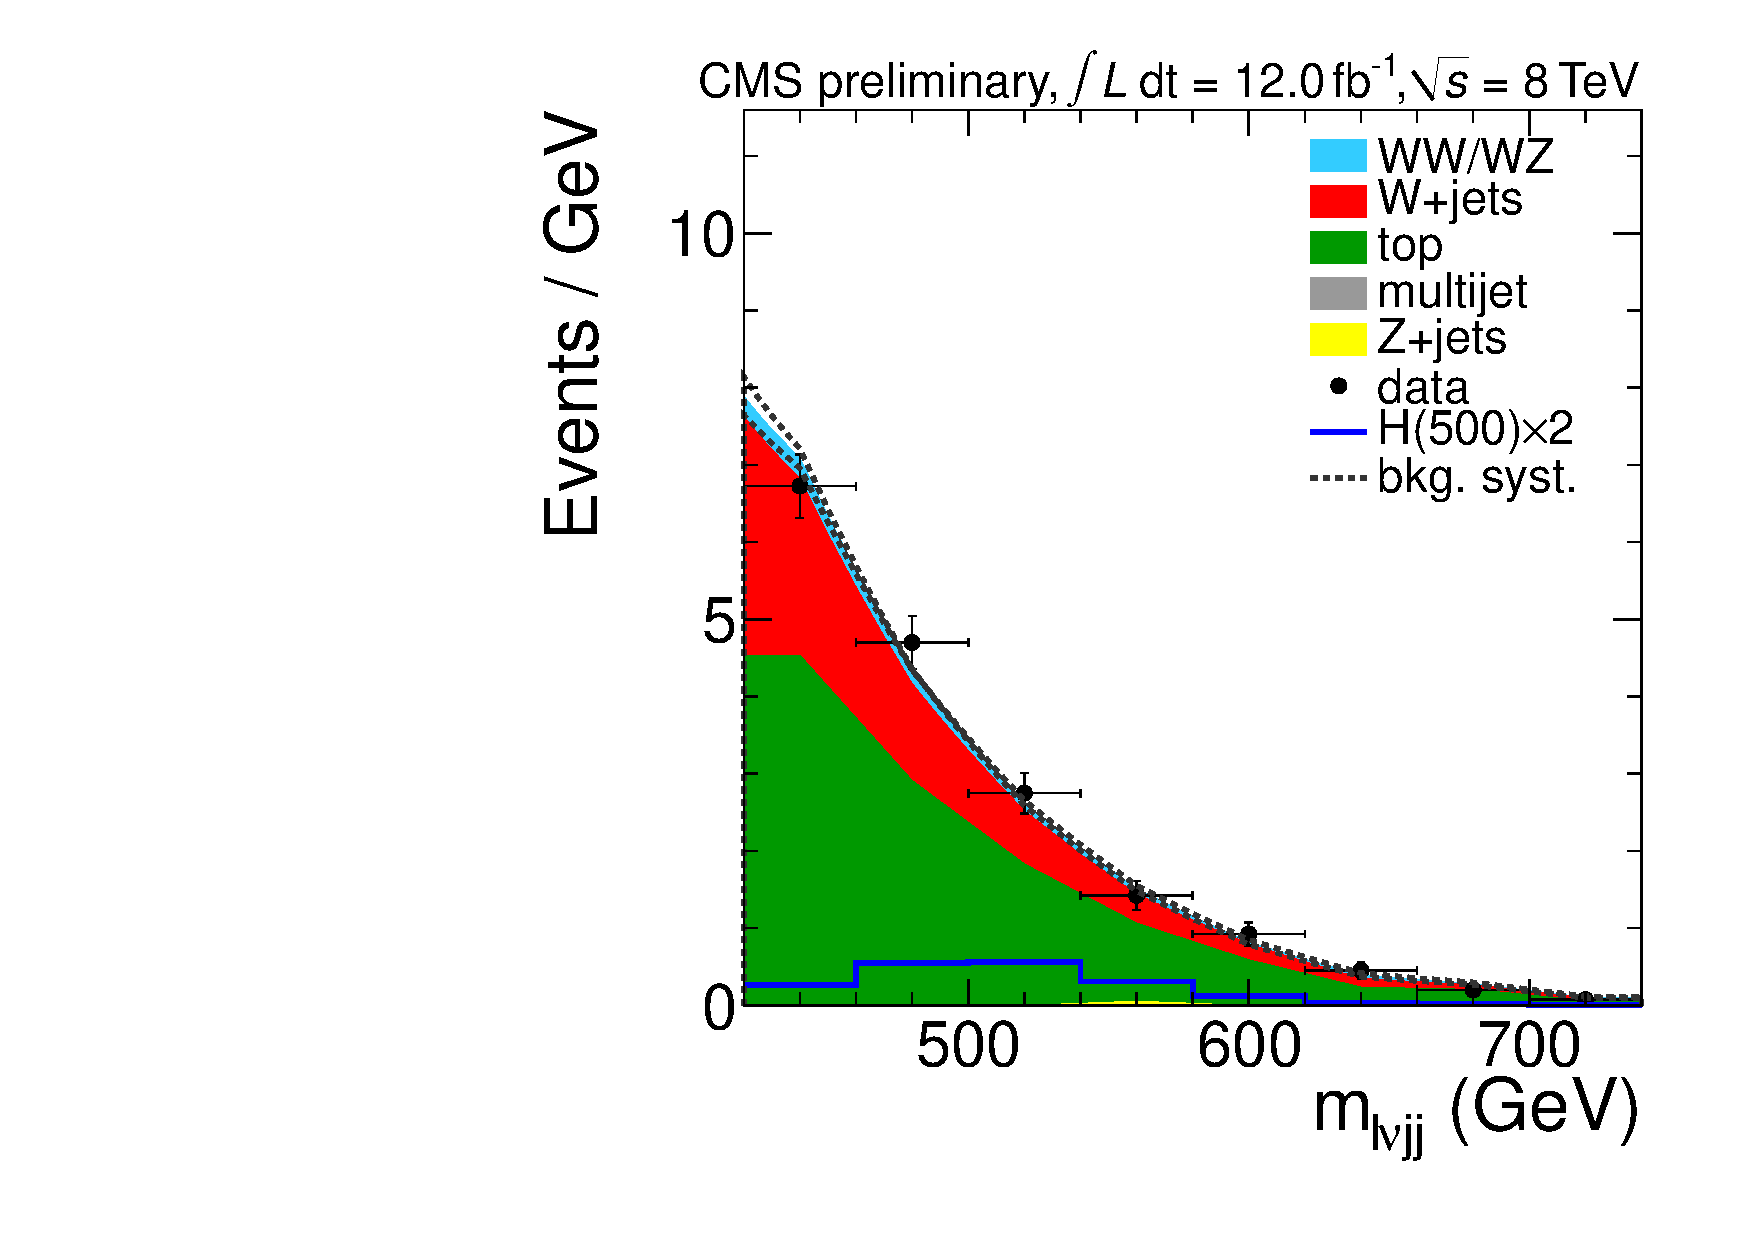
\includegraphics[width=0.45\textwidth]{plots/2012_FOURBSHAPES/H500_Mlvjj_Muon_3jets_Stacked}
     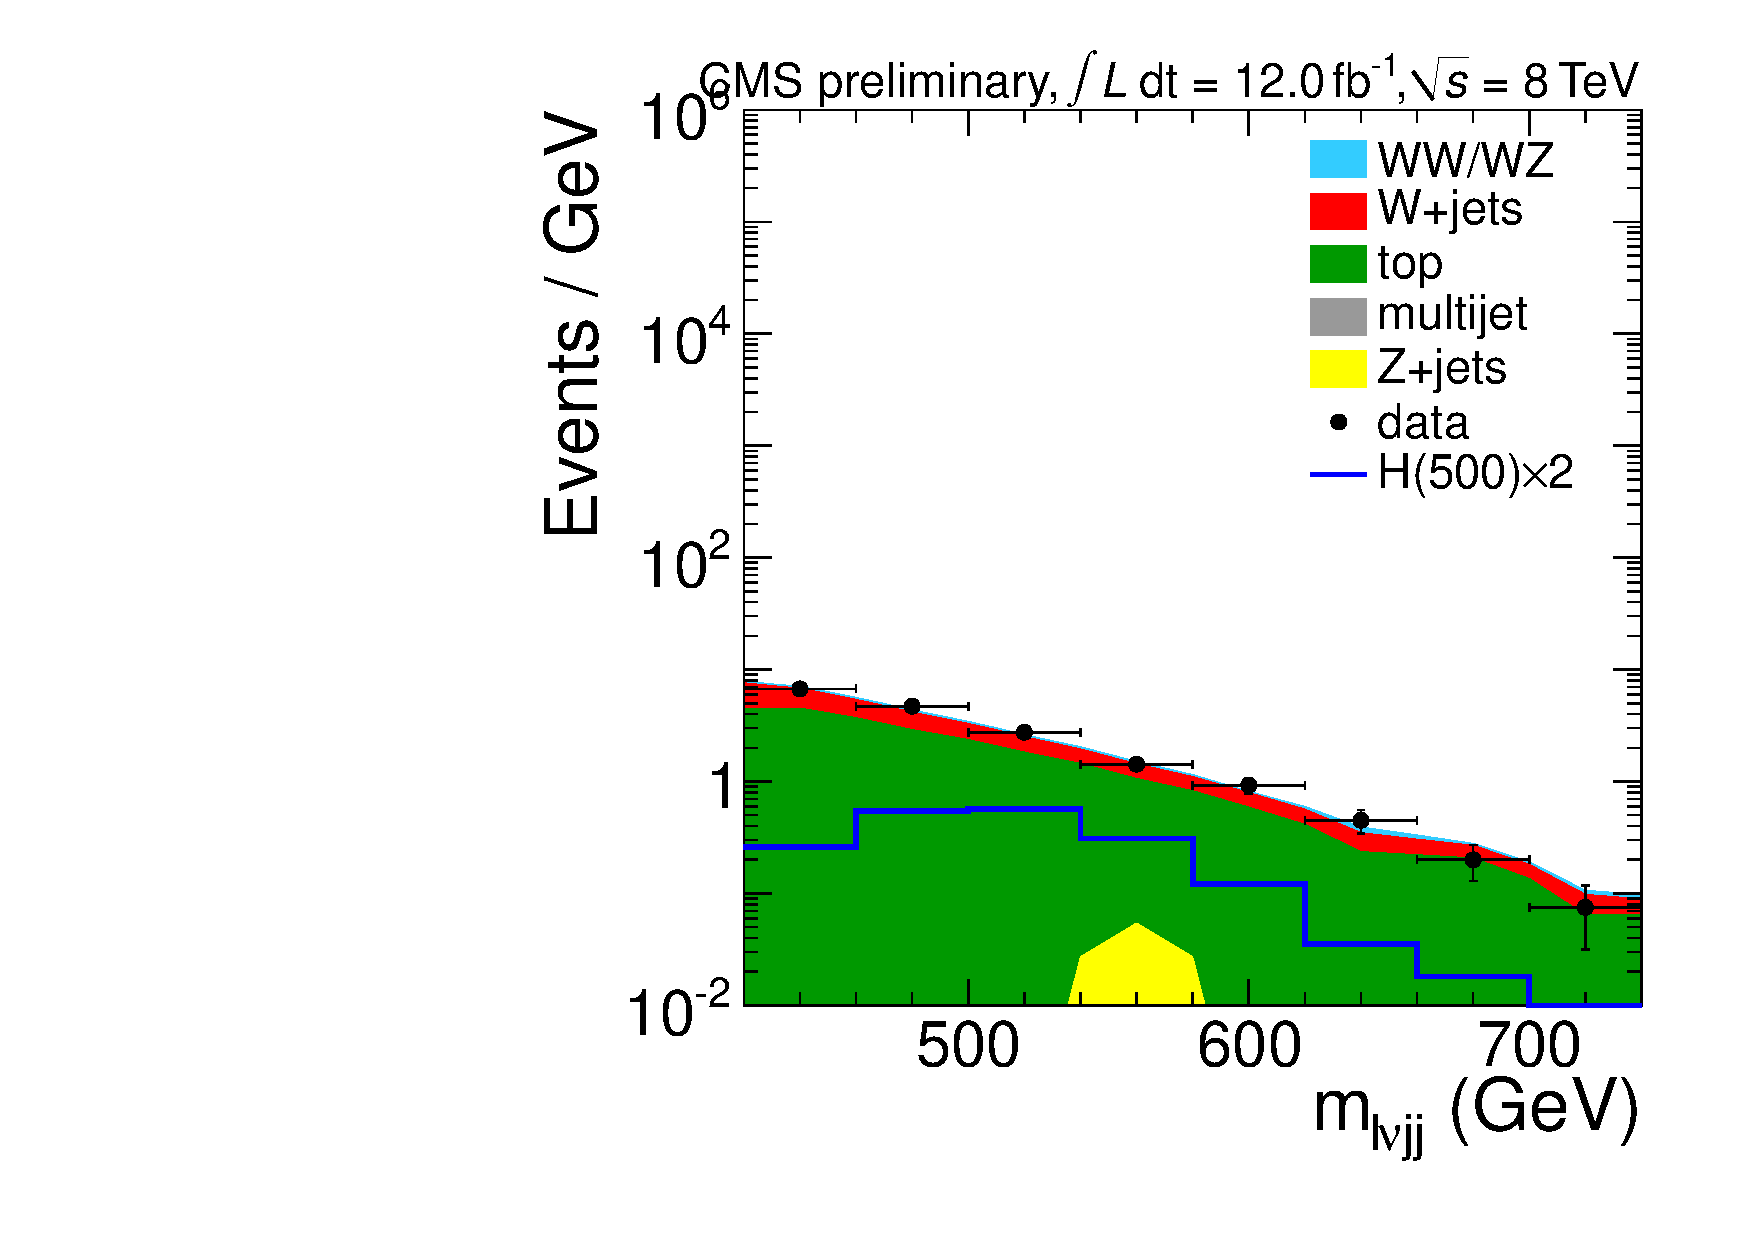
\includegraphics[width=0.45\textwidth]{plots/2012_FOURBSHAPES/H500_Mlvjj_Muon_3jets_Stacked_log}
}
  \caption{The four-body mass distribution of data-driven background events in the signal regions for mass
  point M=500~GeV.}
  \label{fig:m4_dd_example500}
\end{figure}

%The full set of plots for the analysis on the 48 working points can be
%found in the CMS analysis note AN-2012/024, Section 15.

\clearpage
